\documentclass[11pt,a4paper,oneside]{book}

\usepackage{amsmath}
\usepackage{amsfonts}
\usepackage{amssymb}
\usepackage{graphicx}
\usepackage[top=2cm, bottom=2cm, left=3cm, right=2cm]{geometry}
\usepackage{a4wide}
\usepackage[english]{babel}
\usepackage[T1]{fontenc}
\usepackage{amsthm}
\usepackage{url}
\usepackage[utf8]{inputenc}
\usepackage[small,bf,hang]{caption}
\usepackage{fancyhdr}
\usepackage{float}
\usepackage[table]{xcolor}
\usepackage{hyphenat}
\usepackage{lscape}
\usepackage[sectionbib,round]{natbib}
\usepackage{hyperref}

% Custome Page Headers 
\pagestyle{fancy}
\fancyhf{}
\renewcommand{\headrulewidth}{0pt}
\fancyhf[HL]{\nouppercase{\textit{\leftmark}}}
\fancyhf[FC]{\thepage}


% Custom Paragraphs
\setlength{\parindent}{0pt}
\setlength{\headheight}{14pt}
\newcommand{\npar}{\par \vspace{2.3ex plus 0.3ex minus 0.3ex}}
\newcommand{\method}[1]{\texttt{#1}}
\newcommand{\interface}[1]{\texttt{#1}}

\bibliographystyle{plainnat}
\renewcommand{\bibname}{References}

\begin{document}

\frontmatter

\thispagestyle{empty}
\begin{flushleft}
%\vspace{-34.5mm}

\includegraphics[height=40mm]{figs/sedes_2.jpg}\\
\small
KATHOLIEKE\\ UNIVERSITEIT\\ LEUVEN
\end{flushleft}

\vspace*{\stretch{1}}

\begin{center}
\textbf{Software Architecture} \\
\LARGE
\textbf{Phase I: Architecture}
\end{center}

\vspace*{\stretch{1}}

\begin{flushleft}
\small
Kristof Peeters (s0205637)\\
Michiel Staessen (s0188009)
\end{flushleft}

\begin{flushleft}
Prof. W. Joosen \\
Prof. R. Scandariato
\end{flushleft}


% Title details
\title{Software Architecture -- Phase II: Architecture}
\author{Kristof Peeters \and Michiel Staessen}
%\maketitle

% Table of Contents
\tableofcontents

\chapter{Abstract}

\npar This document contains the report of Kristof Peeters and Michiel Staessen
of the second assignment of the course ``Software Architecture'', taught in the
second semester of the first master. The report contains the result of applying
the ADD method on the ReMeS system. Furthermore is the architecture, resulting
from ADD fully documented together with an illustration of several potential
scenarios. Finally a conclusion is given together with an appendix containing
the element catalog and interface catalog.
\chapter{Introduction}

\npar In this project a remote measurement, monitoring and control system
(ReMeS) for utilties such as gas, water and electricity is developed. The
project started with the formulation of the nonfunctional and functional
requirements of this system. In this phase the goal is to design an architecture
which support those requirements. 

\npar This design phase is guided by the attribute driven design method, known
as ADD. Each iteration of this design method is documented in chapter
\ref{chap:add}. The final result can be found in the next chapter,
\ref{chap:final-architecture}. The accompanying interface- and element catalog
can be found in the appendix. In a last chapter the a number of example
scenario's can be found, which are presented as (UML) sequence diagrams.


\mainmatter

% Content
\chapter{Attribute Driven Design}
\label{chap:add}

% Iteration 1
\section{Iteration 1: Decomposition of the whole system}
\label{add:it1}

\npar In the first iteration, the whole system, ReMeS is decomposed. It takes
all the requirements and quality attribute scenarios as input.

\subsection{Step 0: Confirm there is sufficient requirements information} 

% TODO de tekst in deze subsectie beschrijft niet helemaal wat in deze sectie
% moet komen. Ofwel schrappen we dit, ofwel maken we hier nog eens een overzicht
% van de requirements met prioritization door de opdrachtgever en invloed op de
% architectuur. 
% Referenced from: http://www.sei.cmu.edu/reports/06tr023.pdf

\subsection{Step 1: Identify candidate drivers}
\label{add:it1/drivers}

% TODO verwijs naar step 0?

\npar First of all when designing a decomposition for the whole system, the
choice of the drivers is very imortant since it will shape the architecture the
most. Therefore not only is the priority of the client for each quality
attribute scenario taken into account to choose the drivers, but also the impact of
that scenario on the architecure. These impacts are, together with the client
priorities, summarized in table \ref{table:add/it1/priorities}.

\begin{table}
	\begin{center}
		\begin{tabular}{| l | l | l | l | l | l | l | l | l | l |}
		\hline
		\textbf{Quality}			&	Av1	&	Av2	&	Av3	&	P1	&	P2	&	P3	&	M1	&	M2	&	M3	\\
		\hline
		\textbf{Client Priority}	&	H	&	M	&	L	&	H	&	M	&	M	&	H	&	L	&	M	\\
		\hline
		\textbf{Architecture Impact}&	L	&	H	&	L	&	H	&	H	&	M	&	M	&	L	&	M	\\
		\hline
		\end{tabular}
		\caption{An overview of all priorities which are takn into account when
		selecting the architectural drivers.}
		\label{table:add/it1/priorities}
	\end{center}
\end{table}

\npar Off course one wants to maximize the priority in both cases. Based on the
priorities in table \ref{table:add/it1/priorities}, one high priority and two
medium priority quality attribute scenarios are selected as architectural driver. An
overview of the selected drivers and their use cases is given below.

\begin{itemize}
  	\item P1 (High): Timely closure of valves
  	\begin{itemize}
  	  	\item UC8 (High) : send measurement
  		\item UC13 (High): Send alarm 
  	\end{itemize}
  	\item P2 (Medium) : Anomaly detection
  	\begin{itemize}
  	  \item UC10 (Medium) : Detect anomaly %TODO
  	\end{itemize} 
  	\item Av2 (Medium) : Missing measurements %TODO use cases ?
\end{itemize}

\npar The considered use cases includes the use cases listed below. 

\begin{itemize}
	\item UC7 (High): Send trame to remote device
	\item UC9 (High): Notify customer
	\item UC10 (Medium): Detect anomaly
\end{itemize}

\npar The choice of P1 is logical because it has the highest priority available
(both a high client priority and impact on the architecture). The reasons for
selecting P2 and Av2 are more subtle since there are still combinations
available (e.g. Av1) which precede P2 in the priority hierarchy. The choice is
twofold. First of all P2 is very easy to combine with P1 because they both place
constraints on the database access in the two different operate modi (normal and
overload). Second, the impact on the architecture is very high in contradiction
to other high (client) priority requirement such as Av1 or M1. Based on the
second argument there was also opted to go for Av2.

\npar Based on the architectural drivers, the remote module subsystem has to
provide functionality for remote module communication (receiving and sending
trames), trame storage, trame processing and stakeholder communication. 

\npar In order to obtain a better understanding of the relationships between
these functionalities, a small domain model is drafted. Figure
\ref{fig:add/it1/draft} This model can then be refined later on
in this level of decomposition.

\begin{figure}[H]
	\begin{centering}
		% TODO
		%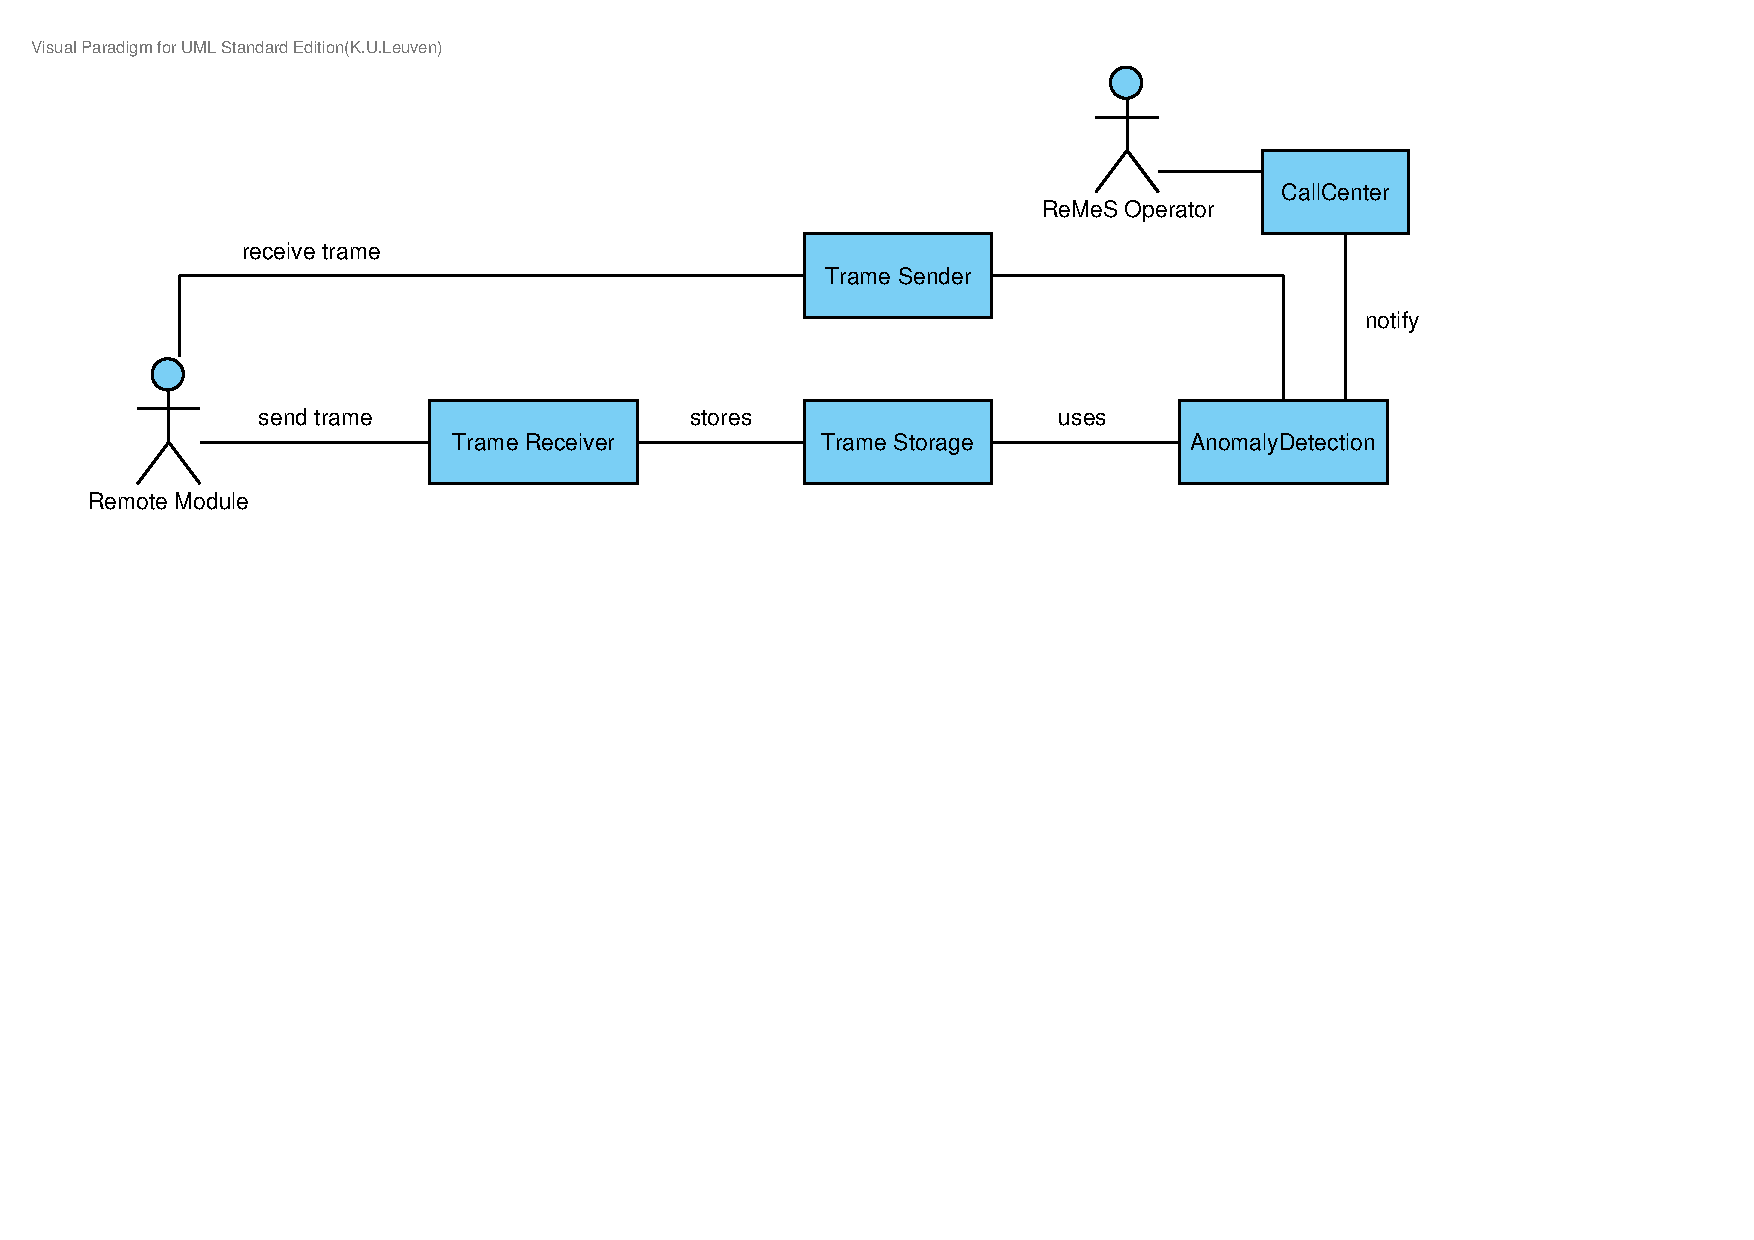
\includegraphics[width=0.6\textwidth]{figs/decomposition/whole-system/domainmodel-draft.pdf}
		\caption{Draft of the domain model used in the level 1 decomposition}
		\label{fig:add/it1/draft}
	\end{centering}
\end{figure}

\subsection{Step 2: Choose design concepts}
\label{add:it1/concepts}

\subsubsection{Tactics}
\label{add:it1/tactics}

\paragraph{Availability}
 
\npar After selecting the drivers for the current decomposition, one has to
choose the tactics to achieve them. Recall from section \ref{add:it1/drivers}
that one of the drivers was Av2. All approaches to maintain availability
involve either detection, recovery or prevention of faults.

\npar First of all, a fault needs to be detected. For this, there are three
options: ping/echo, heartbeat and exceptions. It is important to notice that the
latter is not very practical. This can be illustrated with a simple example.

\npar Suppose that a component $c_1$ depends on another component $c_2$. For
some reason, $c_1$ does not need the services of $c_2$ for a duration longer
than the detection interval of one minute (see Av2). Within this time,
no detection can occur, simply because there is no interaction between the
components. For this reason, we eliminate exceptions as a primary fault
detection system. However, exceptions will still have to be implemented in order
to make the system fail gracefully (a component being unavailable will not
cause the system to crash).

\npar Another detection method uses ping/echo. This primarily focusses on
network connectivity and will not check the availabillity of the service itself.
Again, this is not very practical. A server can be reachable, but the service on
a certain port number may be unavailable. In this case, the ping/echo
method would not detect the fault.

\npar Heartbeat on the other hand, will be part of the system itself and will be
able to check whether the service is still up and running. It will periodically
(at most every one minute) check the state of the system and send out a pulse
to a heartbeat monitor if everything is runnning fine.

\npar Another advantage of using heartbeat is that the pulse can contain data,
more specifically status data. For instance, a single failing disk in a RAID5
array can cause a warning but will not cause the system to crash. This
information can be included in the pulse of the heartbeat to inform the
administrators to replace the failing disk.

\npar As a result, heartbeat seems the best solution to detect faults.

% 
\paragraph{Performance} 

\npar For performance tactics there are three categories: resource
arbitration, resource management and resource demand.

\npar If there is more than one request to gain control over a resource, there
has to be some form of scheduling. By far the most used one is a priority
scheduler where requests are served earlier when they have a higher priority.
This is particulary useful for alarms to still reach the appropriate parties in
time even when the system is in overload mode. 

\npar Secondly there is resource management. To process more than one trame at a
time, concurrency can be introduced. This can be done in various ways. Several
threads can be started on one processor, on separate processors or even on
separate systems. Another possibilitiy is off course increasing the available
hardware but since this is not a very cost effective solution, this is left out
of consideration.

\npar On a lower level one could also try to minimize network overhead by
only sending small amounts of data in each trame. This is achieved by
limiting the size of the trames to 160 bytes.

\npar To conclude a small overview is given of all selected tactics for this
decomposition.

\begin{itemize}
 	\item Av1 (High): Measurement database Failure
 	\begin{itemize}
 		\item Detection: Heartbeat 
 		\item Recovery : Active replication
 	\end{itemize}
  	\item P1 (High): Timely closure of valves
  	\begin{itemize}
  		\item Resource arbitration : Scheduling
		\item Resource management  : concurrency
		\item Resource demand      : limited tramesize
  	\end{itemize}
\end{itemize}

\subsubsection{Design Patterns}
\label{add:it1/patterns}

\paragraph{Active Object}

\npar With respect to resource arbitration and resouce management, the
\emph{Active Object} design pattern is chosen for trame communication and
processing. Schedulers will determine the order in which trames are received,
processed and sent. 

\paragraph{Strategy}

\npar The previously mentioned schedulers will have different scheduling
policies, implemented with the \emph{Strategy} design pattern, in order to
allow operation in different modes.

\npar The trames will have to be objectified. This will yield two advantages.
Firstly, the scheduler can be implemented using the \emph{Command Processor}
design pattern. Secondly, a unified language will exist for all vendor
specific trame formats.

\paragraph{Resource Pool}

\npar To allow load balancing (and hence increase the performance) multiple
instances of the anomaly detection are created . This can be achieved by using
the \emph{Resource Pool} design pattern. 

\paragraph{Shared Repository}

\npar Since several databases will be needed in this iteration, the
\emph{Shared Repository} pattern will be employed to %TODO argumenten ?

\subsection{Step 3: Instantiate architectural elements and allocate responsibilities}
\label{add:it1/elements}

\begin{figure}[H]
	\begin{centering}
		% TODO Figure
		%\includegraphics[width=0.6\textwidth]{figs/decomposition/whole-system/decomposition.pdf}
		\caption{The decomposition of the Outbound Communicatin Scheduler. Iteration
		1}
		\label{fig:add/it1/decomposition}
	\end{centering}
\end{figure}

\subsubsection{Remote Module Communication unit}

\npar This module is responsible for all communication from and to remote
modules (all types of communication and both valves and control devices).
Incoming trames (from remote devices) are handed over to the storage scheduler.
Trames which need to be sent to to remote modules are dispatched to the correct
module through the correct medium.

\subsubsection{Storage Scheduler}

\npar This scheduler gets all incoming trames from remote modules and schedules
them for storage. Dependent on the active scheduling policy trames can be
prioritized over other trames. For instance, an incoming alarm trame for a gas
leak has top priority and has strict bounds on the delivery time (see the
quality attribute scenarios). Furthermore serves this scheduler as a buffer.
This is particularly useful when the storage unit is overloaded.

% \subsubsection{Heartbeat monitor cluster}
%  TODO: verplaatsen of weggooien.
% \npar The heartbeat monitor cluster is the result of the tactic to detect a
% fault, namely heartbeat. This component will monitor all other components to see
% if they are still alive (i.e. not crashed). Off course it is not unthinkable
% that the monitor component fails itself. Therefore this component has to monitor
% itself by for example an extra monitor that monitors the monitor.

\subsubsection{Storage of trames}

\npar This component is responsible for all storage of measurements (and
measurements only). It receives trames from the storage scheduler and notifies
the Anomaly Detection scheduler when a new trame is available.

\subsubsection{Anomaly Detection Scheduler}

\npar When the storage unit has stored a new trame, this scheduler is notified
and fetches the freshly stored trame. Analogous to the other scheduler this
scheduler serves as a buffer to prevent overloading on the anomaly detection
unit. Once again different scheduling policies can be switched on.

\subsubsection{Notification Unit}

\npar This module is contacted by the anomaly detection. When the latter detects
an anomaly in the usage of one the utilities of a customer or a (non false)
alarm, then that customer (and possibly the emergency services) needs to
notified. This is the responsibility of the Notification Unit.

\subsubsection{Anomaly Detection Unit}

\npar The Anomaly Detection unit is responsible for running the algorithms to
discover anomalies. It receives trames from the anomaly detection scheduler so
it can process them. After receiving such a trame, additional trames are fetched
by sending a read query to the storage scheduler. These additional trames
are from the same customer or utility company because the detection algorithms
off course work based on data sets instead of single trames. Notice that there
are multiple instances of this anomaly detection unit. This allows load
balancing, cf. P2.

\npar The task of this unit is the managing of all these instances. This
includes monitoring the load of all the instances, performing the read queries
and distributing the resulting trames. Upon detecting an anomaly two possible
actions (or both) can be undertaken. The first is sealing a valve if it is a
severe leak (this action is represented by the dependency between the outgoing
communication scheduler and the anomaly detection). The second is notifying the
approriate parties (the customer and/or the emergency services).

\subsubsection{Outgoing Communication Scheduler}

\npar The outgoing communication scheduler has as duty the scheduling of
trames which are sent to remote modules. There is a need for scheduling because
control trames to shut a valve need to reach the specified module within certain
time constraints according to P1. This scheduling can again be realized by the
use of different policies.

\subsubsection{Stakeholder Communication unit}

\npar This unit is responsible for all communication towards stakeholders (e.g.
customers, emergencyservices, etc.). 

\subsection{Step 4: Define interfaces for instantiated elements}
\label{add:it1/interfaces}

\subsubsection{Remote Module Communication Unit}

\paragraph{InputTrame} %TODO: parameter van de receive

\npar The remote module communication unit offers one method
\method{receive(\ldots)} which is invoked by remote modules whenever they want
to send a trame towards ReMeS.

\paragraph{OutputTrame}

\npar The output translator also offers only one method, \method{send(trame)}.
This method can be invoked by components who need to communicate with one or
more remote modules.

\subsubsection{Storage Scheduler}

\paragraph{StorageQueryScheduler}

\npar The \interface{StorageQueryScheduler} has one method,
\method{schedule(query)}. This method will feed the given query into the
scheduler. 

\subsubsection{Storage}

\paragraph{TrameCRUD}

\npar This interface offers four methods, summarized CRUD. This abbreviation
stands for : ``Create Read Update Delete'' and refers to the four basic
operations possible on a database.
 
\npar The first method, \method{create(query)}, can be used for the insertion of
a new data table. The \method{read(query)} method serves to read a certain
amount of trames (e.g. all measurements a of certain utility provider or
customer). Third there is an \method{update(query)} method to change the
content of a table (e.g. add a measurement for a certain customer). Finally a
\method{delete(query)} method is provided to delete data.

\subsubsection{Anomaly Detection Scheduler}

\paragraph{DetectionScheduler}

\npar The \interface{DetectionScheduler} interface offers a
\method{schedule(trame)} method which will offer the given trame to the
scheduler.

\subsubsection{Anomaly Detection}

\paragraph{AnomalyDetector}

\npar This interface once again offers only one method \method{detect(trame)}.
Invoking this method can trigger various anomaly detection algorithms to start
running (or add the given trame to an already running algoritm). There can be an
analysis for the utility provider or customer where the measurement belongs too.
These algorithms typically take more than one trame as input so additional
trames may be fetched. Therefore a read query be scheduled through the
\interface{StorageQueryScheduler} by invoking the \method{read(query)} (where
the query off course has to be constructed within the \method{detect} call).

\npar When the outcome of one or more algorithms indicates that an anomaly is
found (or when the initial trame was an alarm trame) the customer and/or emergency
services may have to be notified. Therefore the \method{send(notification)}
of the \interface{NotifyUnit} can be used. This method call will handle the
notification.

\subsubsection{Notification Unit}

\paragraph{NotifyUnit}

\npar The interface this notification unit offers, has one method, namely a
\method{send(notification)}. Invoking this method results in the notification of
the recipient (which is included in the notification parameter) with the actual
message.

\subsubsection{Outbound Remote Module Scheduler}

\paragraph{OutboundTrameScheduler}

\npar To fulfill the scheduling functionality a method is needed where
components can send their trames to. This method is called
\method{schedule(trame)} and feeds the given trame into the scheduler where it
will wait to be redirected to the communication unit.

\subsubsection{Shared Repository} 

\npar All interfaces offered by the shared repository are analogous to the
\interface{TrameCRUD} to a great extent. After all the basis of all of these
interfaces is the CRUD principle.

\paragraph{CustomerProfileCRUD}
%TODO: niet volgens CRUD principe
\npar This interface includes a \method{getCustomerByDeviceId(deviceId)} to
enable the remote communication module to retrieve the customer which belongs to
a certain incoming trame. This customer information can then be used throughout
the system whenever needed.

\paragraph{RemoteModuleConfigurationCRUD}

\npar 

\paragraph{AlarmStorageCRUD}

\npar 

\subsection{Step 5: Verify and refine}
\label{add:it1/verification}

\npar In this step, we verify that that the element decomposition thus far meets
the functional requirements and quality attribute requirements. Also, child
elements are prepared for further decomposition.

\npar Three things have to be verified. First, we will verify that all
functional requirements and quality attribute requirements of the parent element
have been allocated to one or more child elements in the decomposition.
Secondly, all responsibilities that were assigned to child modules are
translated into functional requirements for the individual items and finally,
quality attribute scenarios for individual child elements are refined if
necessary.

\npar We will list all the child elements, together with their allocated use
cases and quality attribute requirements. If a requirement is split or
delegated, it is also mentioned in the list. To conclude an overview is given of
resolved requirements in this iteration.

\begin{itemize}
	\item Communication Unit
	\begin{itemize}
	  	\item UCx : Retrieve Customer from remote module identification %TODO dit
	  	% wordt toegewezen aan communication unit, maar het is wel een oproep van
	  	% een methode op other (``getCustomerby etc)
	  	\item UCy : Retrieve Remote Module protocol
		\item UC7': Send trame to remote device (split)
		\item Av2': Missing measurements (split)
		\item M1' : Dynamic pricing (split)
		\item M2' : Fine-grained metering for enterprises (split)
		\item M3' : Decentralized electricity generation (split)
	\end{itemize}
	\item Storage Scheduler
	\begin{itemize}
		\item P1' : Timely closure of valves (split)
	\end{itemize}
	\item Storage
	\begin{itemize}
		\item Av1: Measurement database failure (delegated)
		\item Av2': Missing measurements (split)
	  	\item P3': Requests to the measurement database (delegated)
	\end{itemize}
	\item Anomaly Detection Scheduler
	\begin{itemize}
		\item UCz: Determine the operational mode (derived)
		\item P1' : Timely closure of valves (split)
	  	\item P2': Anomaly Detection (split)
	\end{itemize}
	\item Anomaly Detection
	\item Customer Communication Unit
	\begin{itemize}
		\item UC9: Notify Customer
	\end{itemize}
	\item Outgoing Communication Scheduler
	\begin{itemize}
	  \item P1' : Timely closure of valves
	\end{itemize}
	\item Other functionality
	\begin{itemize}
	  	\item UC1: Log in
	  	\item UC2: Log off
	  	\item UC3: Register customer
	  	\item UC4: Unregister customer
	  	\item UC5: Associate device to customer
	  	\item UC6: Customize customer profile
	  	\item UC11: Operate remote actuator remotely
	  	\item UC12: Set alarm recipients
	  	\item UC14: Request consumption predictions
	  	\item UC15: Generate invoice
	  	\item UC16: Mark invoice paid
	  	\item UC17: Perform research
	  	\item Av3: Third Party Billing Service failure
	  	\item M1': Dynamic pricing
	  	\item M2: Fine-grained metering for enterprises
	  	\item M3': Decentralized electricity generation
	\end{itemize}
	\item Resolved requirements
	\begin{itemize}
		\item UC7': Send trame to remote device (split)
		\item UC8 : Send measurement
		\item UC13: Send alarm
		\item UC10: Detect anomaly
		\item P1' : Timely closure of valves (split)
		\item P2' : Anomaly detection (split)
	\end{itemize}
	\item 
\end{itemize}


% Iteration 2
\section{Iteration 2: Decomposition of the Remote Module Communication Unit}
\label{add:it2}

\subsection{Step 1: Identify candidate drivers}
\label{add:it2/drivers}

\npar In the previous iteration, four requirements (UC7', Av2', M1' and M3')
were assigned to the remote module communication unit and 2 use cases were
created. The three quality attributes will form the drivers for this iteration.

\subsection{Step 2: Choose design concepts}
\label{add:it2/concepts}

\subsubsection{Tactics}
\label{add:it2/tactics}

\paragraph{Modifiability}

\npar When opting for a modifiable solution 3 main (groups) of tactics can be
used: localize modifications, prevent ripple effect and defer binding time.
Two tactis are picked from the first group, namely abstraction of common
services and anticipate expected changes.

\npar To prevent rippling effects three tactics are employed. The first one,
probably the most important one, is the hiding of information through the use of
interfaces. Furthermore are communication paths restricted and an intermediary
will be used.

\paragraph{Availability}

\npar The chosen availability tactic is detection, more specific the heartbeat
mechanism.

\subsubsection{Design Patterns}
\label{add:it2/patterns}

\npar To realize the modifiability tactics and allow the coverage of UC7', the
\emph{Message Translator} pattern is selected. The translator acts an
intermediary between the remote module and ReMeS and all information remains
hidden behind a simple interface. 

\npar To push this information hiding even further a modified version of the
\emph{Resource Pool} pattern is used. This will be enlightened in the next
section.
%TODO: misschien is dit niet helemaal waar, want resource pool is meer op
% performantie gericht.

\npar Finally the \emph{Publisher - Subscriber} pattern is used to allow
multiple components to receive trames in parallel. 

\subsection{Step 3: Instantiate architectural elements and allocate responsibilities}
\label{add:it2/elements}

\begin{figure}[H]
	\begin{centering}
		% TODO
		%\includegraphics[width=0.6\textwidth]{figs/decomposition/rm-comm-unit/decomposition.pdf}
		\caption{The decomposition of the remote module communication unit. Iteration
		2}
		\label{fig:add/it2/decomposition}
	\end{centering}
\end{figure}

\npar The remote module communication unit has three main components: Input
Translator, Output Translator, Translator Pool, Event Channel, Deadline Monitor
and Trame Consumer. Each of them will be discussed below. As one can see in
diagram \ref{fig:add/it2/decomposition} there are only two communication paths
in the system, one for incoming communication and one for outgoing. In this way
another tactic is realized, namely the restriction of communication paths.

\npar In the previous section there was the mentioning of a modified version of
the \emph{Resource Pool} pattern. One can see this pattern in the usage of the
translator pool. The translator pool component itself acts as a sort of manager
of the pool and handles incoming requests for translators based on a
certain module. The difference with the original pattern lies in the 
diversity of the translators. Each translator is different whereas the
resources normally should all be equal. 

\subsubsection{Input Translator}

\npar The input translator has as duty the translation of incoming (raw) trames
into objectified trames. Therefore it must know what the incoming data format
is. To realize this, it has a translator pool at its disposal where, based on
the module (type) a translator can be fetched. The translated trame is provided
with extra information concerning the customer (i.e. the owner of the module where the
trame came from). When the trames are translated they are published on the event
channel for all interested parties.

\subsubsection{Output Translator}

\npar This component is analogous to the input translator off course. This
component retrieves the right translator from the pool based on the module
where the incoming trame should be send to. It is important to notice that all
outgoing communication towards remote modules goes through this module.

\subsubsection{Translator Pool}

\npar The translator pool acts as the manager for the pool and all requests from
both the translators will pass through this component. 

\subsubsection{Event Channel}

\npar The event channel is the communication entity where publishers can publish
events on and subscribers can subscribe on.

\subsubsection{Deadline Monitor}

\npar The responsibility of this process is the monitoring of all bypassing
measurements and guaranteeing that a missing measurement is detected within the
demanded time limits. This monitor is subscribed to the event channel to receive
trames. To guarantee these limits the monitor keeps a table with expected
arrival times of all remote devices which is frenquently checked. Notice that to
protect from failures, this table is made persistent. When a deadline is
exceeded this is stored in the corresponding database. When a certain number of
deadline violations is reached a ReMeS operator is notified. Notice that this
component is in fact the realization of the heartbeat tactic. 

\subsubsection{Trame Consumer}

\npar The trame consumer is a simple forwarding unit which is subscribed to the
event channel and receives all trames which are published on it. It simply
forwards all trames to the storage scheduler.

\subsection{Step 4: Define interfaces for instantiated elements}
\label{add:it2/interfaces}

\subsubsection{Input Translator}

\paragraph{InputTrame} %TODO: parameter van de receive

\npar this interface was already discussed in iteration 1, see section
\ref{add:it1/interfaces}.

\subsubsection{Output Translator}

\paragraph{OutputTrame}

\npar this interface was already discussed in iteration 1, see section
\ref{add:it1/interfaces}.

\subsubsection{Translator Pool}

\paragraph{TranslatorManager}

\npar The translator pool interface offers one method,
\method{GetTranslatorFor(RemoteDevice) : Translator}. This method does nothing
else than return the correct translator for the given remote device (there can be
differences between remote module types, communication channels, etc.).

\paragraph{Translator} %TODO return parameters van translate methodes

\npar Each of the different translators implements the \interface{Translator}
translator interface. This interface includes two methods:
\method{translateFromDevice(RemoteModule)} and
\method{translateToDevice(RemoteModule)}. The former serves as translate method
for the input translator and vice versa for the latter one.

\subsubsection{Trame Event Channel}

\paragraph{TrameChannel} %TODO parameter en return type van publish methode
% (moet dezelfde zijn als het return type van translateFromDevice)

\npar This interface offers two methods as prescribed by the \emph{Publisher -
Subriber} pattern, \method{publish(event)} and \method{subscribe(Filter) :
Void}.

\subsubsection{Deadline Monitor}

\paragraph{TrameNotifiable}

\npar This interface complements the \interface{TrameChannel} interface. When a
component is subscribed to a certain event flow, the channel has to be able to
notify the component when a new event is available. Therefore this interface
offers a \method{notify() : Void}.

\subsubsection{Trame Consumer}

\npar This unit offers the exact same interface as the deadline monitor.

%TODO: hoe zit het met de interfaces tussen de pool en zijn instances ?

\subsection{Step 5: Verify and refine}
\label{add:it2/verification}

\npar All the drivers were resolved so no futher decomposition of any of these
modules has to take place because there are no more requirements to divide
amongst the components. 


% Iteration 3
\section{Iteration 3: Decomposition of the Measurements Database Scheduler}
\label{add:it3}

\subsection{Step 1: Identify candidate drivers}
\label{add:it3/drivers}

\npar Remote measuring is the core business of the ReMeS system. Almost all
components in the ReMeS system need access to the measurements database.
However, not all queries on that database should be treated equally. For
instance, research queries have a lower priority than anomaly detection history
queries (see P3). Therefore, queries to the measurements database need to be
scheduled.

\npar The decomposition of this iteration is driven by

% TODO Drivers herzien en use cases oplijsten

\begin{itemize}
  	\item Av1: Measurements database failure. In case the database goes down, at
  	least 3 hours of measurement data should be stored.
	\item P2': Anomaly detection: Anomaly detection will be triggered for every
	incoming measurement trame. Measurement trames will also have a higher
	priority because incoming trames should be fully processed within a bounded
	time.
	\item P3': Requests to the measurements database: These queries are subjected
	to a maximal execution time based on the SLA. 
\end{itemize}

\subsection{Step 2: Choose design concepts}
\label{add:it3/concepts}

\subsubsection{Tactics}
\label{add:it3/tactics}

% TODO detection?

\npar The scheduler was introduced in iteration 1 (see section \ref{add:it1}) to
improve performance. At the level of the scheduler, performance is determined by
the scheduling policy. 

\npar The scheduling policy is defined by the quality attributes but the
scheduler itself can be implemented in different ways. One could use a single
queue for the scheduler. Jobs are pushed on a queue and popped off when the
scheduler can process a new job. 

\npar A scheduler can also be implemented with multiple queues. For each kind of
job, there is a seperate queue. In this case, you would end up with a number of
queues for different priorities. Whenever a job resides in a queue for a long
time, it is promoted to a higher priority queue. 

\npar A scheduler must also guarantee that there will be no starvation among
jobs. Starvation happens when a job cannot execute because there always is a
job with a higher priority. When using a first in, first out policy, starvation
will not occur. However, when the database goes into overload mode, this might
become an issue. 

\npar To address this issue, a dynamic priority scheme will be used. The
priority of every job will be increased periodically. In this way, low priority
jobs will eventually have a high priority. 

\subsubsection{Design Patterns}
\label{add:it3/patterns}

\paragraph{Collections for States}

\npar The collections for states design pattern describes a way to efficiently
implement a scheduler with multiple queues. In a client, every state is
represented by a collection of objects with that state. The collections for
each state would be implemented with queues and the the states would represent
priority levels.

\paragraph{Strategy}

\npar If the scheduler allows for multiple policies, the strategy design pattern
can be used to implement these policies. The behaviour of the message router
will be determined by the policy.

\paragraph{Monitor} 

\npar Because the queues can be accessed by both the scheduler and the message
router, monitors have to be put in place to provide synchronization. This is
done to make sure that there aren't any concurrency issues within the scheduler. 

\paragraph{PriorityQueue}

\npar This is not a design pattern but a data type. This queue allows elements
to be inserted with a given priority. This could simplify the design by merging
all queues into one big queue.

\npar There is not really an advantage in having multiple queues. There is only
one instance that can process the jobs. The overhead of comparing the top
entries of the queues might also be large, making this solution less efficient. 

\subsection{Step 3: Instantiate architectural elements and allocate responsibilities}
\label{add:it3/elements}

%      |
%      schedule(QueryCommand):void
%      |
%      v
%    [Scheduler]
%      |
%      schedule(QueryCommand,PriorityQueue):void
%      |
%      v
%    [PriorityQueue]
%      |
%      enqueue(QueryCommand):void
%      |
%      v
%    [Policy]
%      ^
%      |
%      pop() : Query
%      |
%   [QueueReader]
%      |
%      execute(QueryCommand):void
%      |
%      v
%   [TrameStorage]

\npar The decomposition of this component is shown in figure
\ref{fig:it3/elements}. 

\begin{figure}[H]
	\begin{centering}
		%\includegraphics[width=0.8\textwidth]{figs/add/it3/elements.pdf}
		\caption{Overview of the instantiated child components of the Trame Storage
		Scheduler.}
		\label{fig:it3/elements}
	\end{centering}
\end{figure}

\npar All requests to the Measurements Database Scheduler are encapsulated as
QueryCommand objects. These objects have already been created in another
component and represent a query to the measurements database. Because the
scheduling makes communication asynchronous, the QueryCommand contains a
Callback to return the result of the query to the issuer.

\npar The scheduler (MeasurementsScheduler) handles every incoming command
(QueryCommand) by inserting the command in a queue (MeasurementsQueue) with a
certain priority using a policy (MeasurementsPolicy). The scheduling policy
determines the priority of the command based on the nature of that command. The
priorities of all other commands are increased every time a new command is
inserted. This is done to prevent starvation.

\npar An additional component (QueueReader) will pop the command with the
highest priority off the queue and present it on the database for execution. 

\subsection{Step 4: Define interfaces for instantiated elements}
\label{add:it3/interfaces}

\subsubsection{MeasurementsScheduler}

\npar The MeasurementsScheduler provides an interface
\interface{MeasurementSchedulerAPI}. This interface contains a method
\method{shedule(QueryCommand) : void} to schedule new commands.

\subsubsection{MeasurementsPolicy}

\npar The QueryCommand will be placed in the MeasurementsQueue by a Policy.
Therefore, Policy provides an interface \interface{MeasurementsPolicyAPI} which
contains a method \method{insertCommand(QueryCommand, PriorityQueue) : void}.

\subsubsection{MeasurementsQueue}

\npar The MeasurementsQueue must provide methods for inserting items and
removing items. These methods are contained in the
\interface{MeasurementsQueueAPI} and are called
\method{insertCommand(QueryCommand, priority : Double) : void} and
\method{remove() : QueryCommand}. The first method is used by the
MeasurementsPolicy and the last one is used by the MeasurementsQueueReader.

\npar Figure \ref{fig:it3/interfaces} summarizes the components and the
interfaces instantiated in this iteration.

\begin{figure}[H]
	\begin{centering}
		%\includegraphics[width=0.8\textwidth]{figs/add/it3/interfaces.pdf}
		\caption{Overview of the interfaces and components of the Trame Storage
		Scheduler.}
		\label{fig:it3/interfaces}
	\end{centering}
\end{figure}

\subsection{Step 5: Verify and refine}
\label{add:it3/verification}

% TODO Verify na herziening drivers.

\npar All quality and functionality is handled in this decomposition.  

\begin{itemize}
	\item P1': Timely propagation of alarm trames is handled by smart Queue
	insertion by the Message Router. 
	\item P2': Timely propagation of measurement trames is also handled by smart
	Queue insertion by the Message Router. 
	\item P3': Potential prioritization of certain database queries. 
\end{itemize}


% Iteration 4
\section{Iteration 4: Decomposition of the Storage Unit}
\label{add:it4}

\subsection{Step 1: Identify candidate drivers}
\label{add:it4/drivers}

\npar This iteration is driven by

\begin{itemize}
	\item Av1: Measurement database failure. The measurements database should be up
	and running 99.9\% of all time. 
	\item Av2': Missing measurements. A failing internal communication component
	should be detected autonomously. 
  	\item P3': Requests to the measurement database. The requests should be
  	handled within a bounded time. 
\end{itemize}

\subsection{Step 2: Choose design concepts}
\label{add:it4/concepts}

\subsubsection{Tactics}
\label{add:it4/tactics}

\paragraph{Availability} 

\npar Av1 states that a 99.9\% uptime must be realized. In order to guarantee
this, three things must be taken into consideration. It should be able to detect
the problem, there should be a way to fix the problem and last but certainly not
least, there should be preventive measures.

\npar There are many alternatives to address availability. The most frequently
used ones are active redundancy, passive redundancy and spare. The main
criterion to select one of these is the downtime of the system. For every
scheme, the downtimes are respectively in the order of milliseconds, seconds and
minutes. An uptime of 99.9\% corresponds to 0.72 hours (= 43.2 minutes) of
permitted downtime on a monthly basis. This number reveals potential problems
for when a spare is used because there can be only less than 10 failures a
month. For this reason, use of spares is eliminated.

\npar The difference between active and passive replication is rather subtle.
In an active replication scheme, the system will recover faster then in a
passive replication scheme but all replicas should be in a consistent
state. This will increases communication overhead in comparison with the
passive replication scheme.

\npar On the other hand, the active replication scheme can also provide load
balancing for read-only queries. If one replica has a lower load than any other,
that replica can be used to process the query. Because of this advantage, the
active replication scheme is selected.

\subsubsection{Design Patterns}
\label{add:it4/patterns}

\paragraph{Replicated Component Group} 

\npar To make the data highly available, the database will be replicated. This
can be achieved by using the \emph{Replicated Component Group} design pattern.
The database access will be replaced with a front-end interface that replicates
all write queries to all the replicas and load balances read queries over all
instances.

\subsection{Step 3: Instantiate architectural elements and allocate responsibilities}
\label{add:it4/elements}

\npar A FrontEnd will provide an interface to execute queries on the
measurements database. The FrontEnd will also manage all instances of the
measurements database.

\subsection{Step 4: Define interfaces for instantiated elements}
\label{add:it4/interfaces}



\subsection{Step 5: Verify and refine}
\label{add:it4/verification}

% Iteration 5
\section{Iteration 5: Decomposition of the Scheduler for Anomaly Detection}
\label{add:it5}

\subsection{Step 1: Identify candidate drivers}
\label{add:it5/drivers}

\npar This iteration is driven by:

\begin{itemize}
	\item P1': Timely closure of valves.
	\begin{itemize}
  		\item Alarm trames have to be handled within a bounded time. 
    \end{itemize}
	\item P2': Anomaly Detection.
	\begin{itemize}
	  \item When the system is in overload modus the processing order of trames
	  occurs on a priority basis (premium service has a higher priority than
	  normal service).
	\end{itemize}
\end{itemize}

\npar No use cases were delegated to this component.

\subsection{Step 2: Choose design concepts}
\label{add:it5/concepts}

\npar The design concepts for this decomposition are completely analogous to the
design concepts of iteration 3 (see section \ref{add:it3/concepts}). 

\subsection{Step 3: Instantiate architectural elements and allocate responsibilities}
\label{add:it5/elements}

\npar Also analogous to iteration 3 (see \ref{add:it3}), an ADScheduler will
enqueue processing jobs with a priorities in an ADQueue with an ADPolicy. An
ADQueueReader will dequeue jobs from the queue en feed them
to the Anomaly Detection Unit. 

\npar An overview of the instantiated child components of the Anomaly Detection
Scheduler is shown in \ref{fig:it5/elements}.

\begin{figure}[H]
	\begin{centering}
		% TODO Figure
		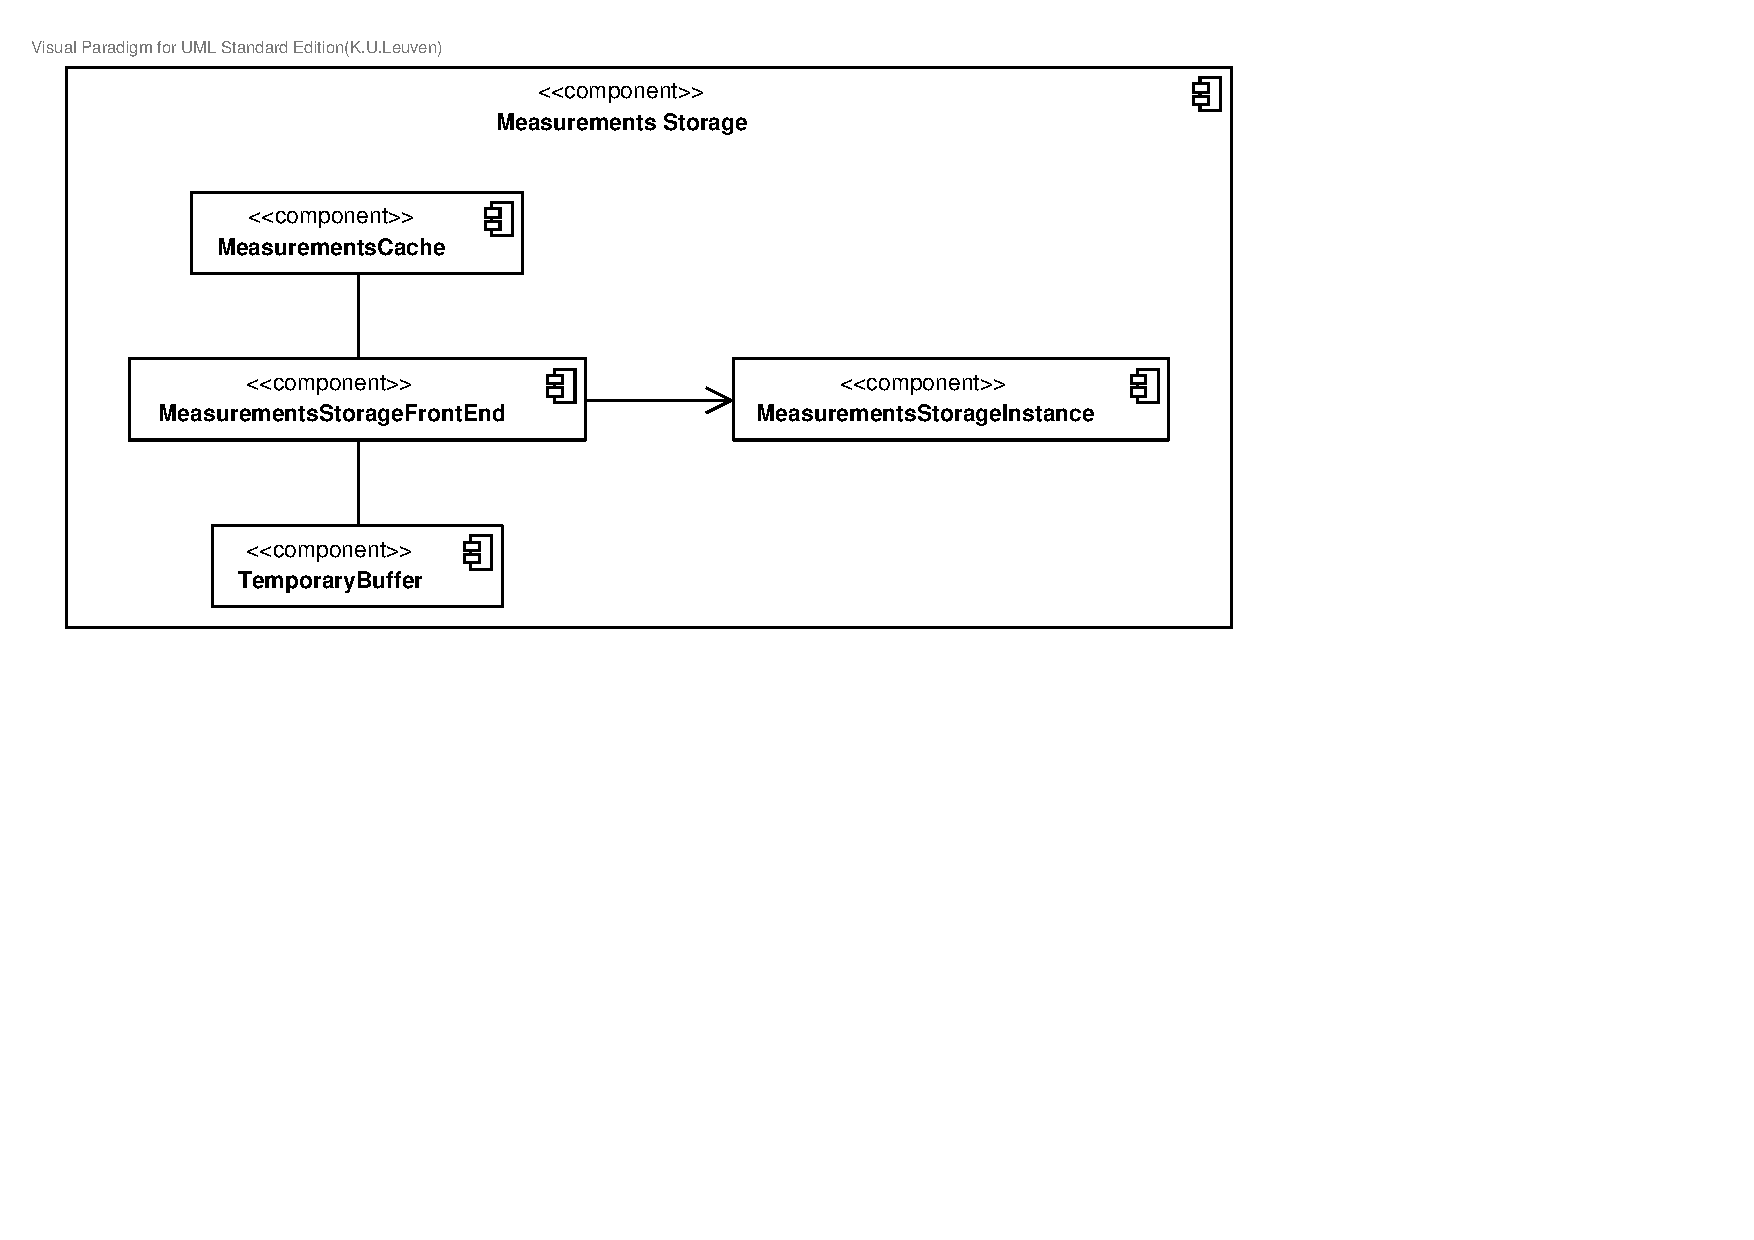
\includegraphics[width=\textwidth]{figs/add-it4-elements.pdf}
		\caption{Overview of all instantiated child elements in the Anomaly
		Detection Scheduler}
		\label{fig:it5/elements}
	\end{centering}
\end{figure}

\subsection{Step 4: Define interfaces for instantiated elements}
\label{add:it5/interfaces}

\npar Because this scheduler is very similar to the measurements scheduler from
iteration 3 (see \ref{add:it3}), the interfaces are also very similar. 

\npar Analogous to iteration 3, jobs are given in the form of ADCommands. An
ADCommand is an encapsulation of an anomaly detection request. This object
contains a copy of the received trame and the necessary data to fetch the
historical measurement data, the alarm data and the configuration data for this
device. This data will be used to determine whether an alarm is a false positive. 

\subsubsection{ADScheduler}

\npar The ADScheduler provides an interface
\interface{ADSchedulerAPI}. This interface contains a method
\method{shedule(ADCommand) : void} to schedule new commands.

\subsubsection{ADPolicy}

\npar The ADCommand will be placed in the ADQueue by a policy. Therefore,
ADPolicy provides an interface \interface{ADPolicyAPI} which contains a method
\method{insertCommand(ADCommand, ADQueue) : void}.

\subsubsection{ADQueue}

\npar The ADQueue must provide methods for inserting items and removing items.
These methods are contained in the \interface{ADQueueAPI} and are called
\method{insertCommand(ADCommand, priority : Double) : void} and \method{remove()
: ADCommand}. The first method is used by ADPolicy and the last one is used by
ADQueueReader.

\npar Figure \ref{fig:it5/interfaces} summarizes the components and the
interfaces instantiated in this iteration.

\begin{figure}[H]
	\begin{centering}
		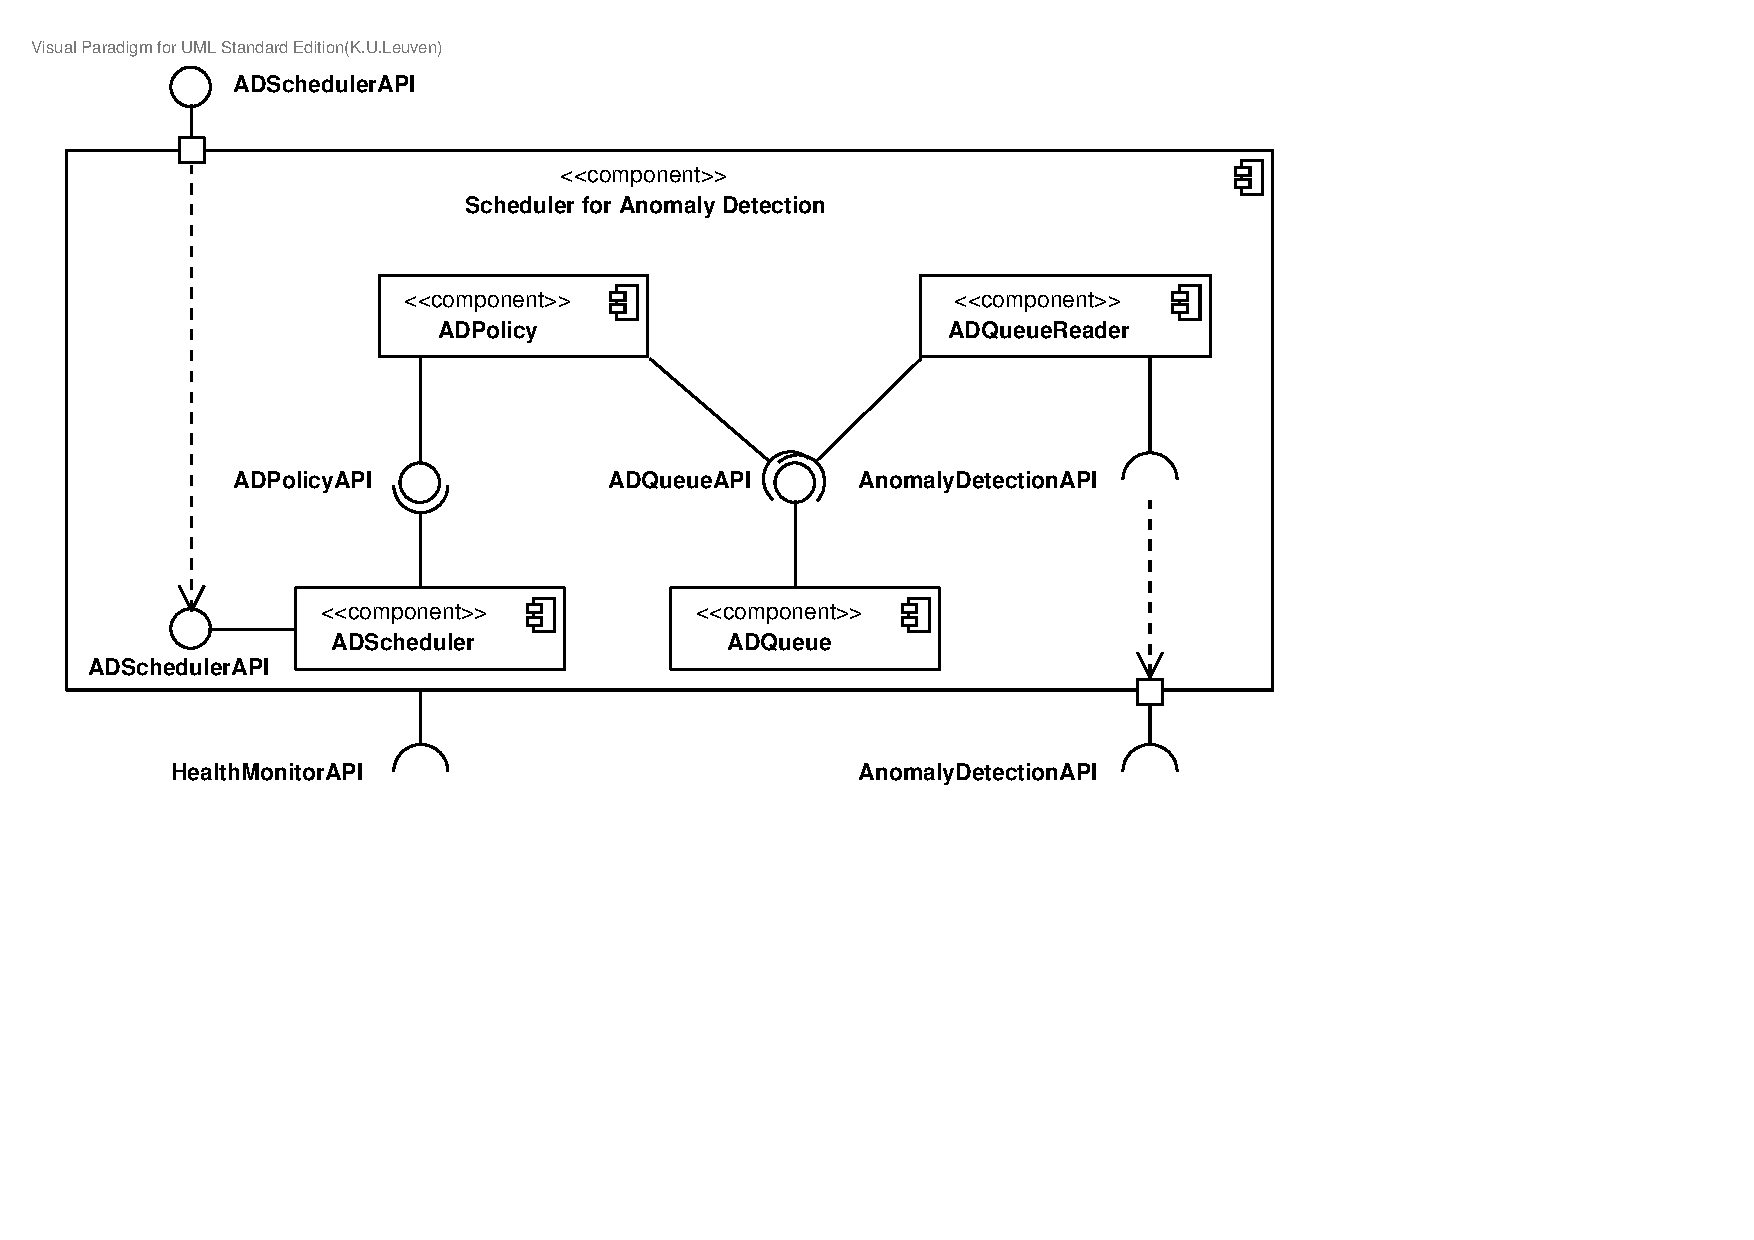
\includegraphics[width=\textwidth]{figs/add-it5-interfaces.pdf}
		\caption{Overview of the interfaces and components in the Anomaly Detection
		Scheduler}
		\label{fig:it5/interfaces}
	\end{centering}
\end{figure}

\subsection{Step 5: Verify and refine}
\label{add:it5/verification}

% TODO verify & refine


% Iteration 6
\section{Iteration 6: Decomposition of the Outbound Communication Scheduler}
\label{add:it6}

\subsection{Step 1: Identify candidate drivers}
\label{add:it6/drivers}

\npar It is crucial that ``shut down valve" trames are sent in time to the
correct module considering that trames who arrive to late can ultimately
lead to a potential disaster claiming the lifes of several people. Therefore the
trames for outbound communication (i.e. towards modules) need to be
scheduled. Therefore P1 was delegated to this scheduler and will be the
(only) driver of this iteration.

\subsection{Step 2: Choose design concepts}
\label{add:it6/concepts}

\npar The design concepts for this decomposition are exactly the same as those
of the storage scheduler, see section \ref{add:it3/concepts}. This is logical
considering that both schedulers are established with performance drivers in
mind.

\subsection{Step 3: Instantiate architectural elements and allocate responsibilities}
\label{add:it6/elements}

\begin{figure}[H]
	\begin{centering}
		% TODO
		%\includegraphics[width=0.6\textwidth]{figs/decomposition/outbound-comm-scheduler/decomposition.pdf}
		\caption{The decomposition of the Outbound Communicatin Scheduler. Iteration
		6}
		\label{fig:add/it6/decomposition}
	\end{centering}
\end{figure}

\subsubsection{Message Router}
%TODO: wat voor input formaat krijgt deze module, trames ?
\npar The message router will dispatch incoming trames to the correct queue
based on the importance of the trame and the current policy (the latter is
determined by the system load). 

\subsubsection{Scheduler}

\npar The task of this component is twofold. First of all it does the actual
scheduling. This means that it pops elements out of the priorityqueue to
redirect for further processing (this off course occurs only when the database
is not processing another trame). Second of all, to prevent starvation
priorities are periodically boosted.

\subsubsection{PriorityQueue}

\npar This component represents a multilevel queue. When one keeps the indeces
of the last element of every possible priority, it is easy to insert new trames
according to the current policy and the priority of the trame itself.

\subsection{Step 4: Define interfaces for instantiated elements}
\label{add:it6/interfaces}

\subsubsection{Message Router}

\paragraph{OutboundTrameScheduler}

\npar The OutboundTrameScheduler was already discussed in section
\ref{add:it1/interfaces}.

\subsubsection{Scheduler}

\npar This component offers no interface.

\subsubsection{PriorityQueue}

\paragraph{OutboundQueueu}

\npar This interface is analogous to the priorityqueue interface of the storage
scheduler, see section \ref{add:it3/interfaces}. It offers a \method{pop(trame)}
and \method{push{trame}} method which will respectively pop and push a given
trame from the priorityqueue.

\subsection{Step 5: Verify and refine}
\label{add:it6/verification}

\npar The driver of this iteration, P1, is resolved.

% Iteration 7
\section{Iteration 7: Decomposition of the Notification Unit}
\label{add:it7}

\subsection{Step 1: Identify candidate drivers}
\label{add:it7/drivers}

\npar There is only very little functionality delegated to this unit, namely one
use case, UC9. Since there are no quality attributes this use case will be the
driver of this iteration.

\subsection{Step 2: Choose design concepts}
\label{add:it7/concepts}

\subsubsection{Tactics}
\label{add:it7/tactics}

\npar Since there are no applicable quality attributes in this iteration. There
are no tactics selected. Off course are general OO design principles such as
separation of concerns taken into account as much as possible.

\subsubsection{Design Patterns}
\label{add:it7/patterns}

\npar No patterns were found to develop the functionality of UC9.

\subsection{Step 3: Instantiate architectural elements and allocate responsibilities}
\label{add:it7/elements}

\begin{figure}[H]
	\begin{centering}
		% TODO
		%\includegraphics[width=0.6\textwidth]{figs/decomposition/notification-unit/decomposition.pdf}
		\caption{The decomposition of the notification unit. Iteration 7}
		\label{fig:add/it7/decomposition}
	\end{centering}
\end{figure}

\npar There are 2 main components in this decomposition, the communication
client and the transport pool. Both of them will be explained below. A graphical
illustration is given in figure \ref{fig:add/it7/decomposition}.

\subsubsection{Communication Client} 
%TODO: voor de emergency services moet er misschien een shortcut voorzien worden
% ipv de overhead om nog eerst het communication channel op te zoeken ? 
\npar This component gets the initial notification message. It's task is
twofold. First of all this component has to fetch the communication channel
through which it has to contact the stakeholder (i.e. the emergency services
and/or one or more customers). Therefore it uses the \interface{CustomerProfile}
interface of the database which contains all user information. Secondly, once
the channel is acquired it has to contact the transport pool to ask for the
right transport unit which can be used to send the notification. The transport
pool offers therefore an \interface{Transport} interface.

\subsubsection{Transport Pool}

\npar The transport pool is the manager of several transport components. The
pool will return the right transport component based on the request. Each
transportcomponent is responsible for communication towards the stakeholders
through a specific channel. To realize this, each of these transport components
offers a \interface{Notify} interface. By splitting the transport into different
components the sending of notifications can be parallelized (i.e. over
different communication channels).

\subsection{Step 4: Define interfaces for instantiated elements}
\label{add:it7/interfaces}

\subsubsection{NotifyUnit}
%TODO: gaat de prof niet zagen over wat die message parameter nu juist is ? moet
% ik er misschien nog expliciet bij zetten dat dit een formaat is dat gelijk moet zijn
% voor de AD, De communication scheduler en deze unit ? 
\npar The interface this notification unit offers, has one method, namely a
\method{send(trame)}. Invoking this method results in the notification of the
included recipient with the message also contains in the message parameter.

\subsubsection{Transport}

\npar The transport pool offers the \interface{Transport} interface. It contains
only one method, \method{getTransport(CommunicationChannel)}. This method has to
return the right transport entity based on the communicationChannel parameter.

\subsubsection{Notify}

\npar This last interface also offers just one method, namely
\method{send(message)}. Notice that this method has the same semantics as the
method of the {NotifyUnit} interface, but now the communication channel is known
so the notification can physically take place.

\subsection{Step 5: Verify and refine}
\label{add:it7/verification}

\npar The driver of this iteration, UC9, is resolved. All the steps of its main
scenario are now tracable in the diagram.


% Iteration 8
\section{Iteration 8: Decomposition of Other}
\label{add:it8}

\subsection{Step 1: Identify candidate drivers}
\label{add:it8/drivers}

\npar In the first iteration there were quite a lot of requirements delegated to
this component. This requires some selection to take place. This selection is
once again based on the priorities of the quality attributes. However since all
the remaning quality attribute scenarios are (split versions from)
modifiability, they can be easily combined. Therefore the drivers for this
iteration are M1', M2 and M3'. 

\npar M3' is linked with the following use cases:

\begin{itemize}
  \item UC14: Request consumption predictions
  \item UC15: Generate invoide
  \item UC16: Mark invoice paid
\end{itemize}

\npar Because of this relation between M3' and the listed use cases their
functionality will all be adressed.

\subsection{Step 2: Choose design concepts}
\label{add:it8/concepts}

\subsubsection{Tactics}
\label{add:it8/tactics}

\paragraph{Modifiability}

\npar For the purpose of modifiability three tactics are selected: anticipate
expected changes, the hiding of information and the use of an intermediary.

\subsubsection{Design Patterns}
\label{add:it8/patterns}

\paragraph{Publisher - Subscriber}

\npar The \emph{Publisher - Subscriber} pattern is in this context particularly useful due to
the inherently unknown parties potentially interested in certain messages. E.g. When
later in time dynamic pricing is introduced it is simply possible for the other
interested parties (customers, HAS, etc.) to subscribe to these events. So this
pattern aids in realizing the anticipate expected changes tactic.

\paragraph{Facade}

\npar To shield the system and it's external actors (i.e. The third party
billing service and utility providers) the \emph{Facade} pattern is interesting.
The pattern suggests a single point of access for both of the aforementioned
actors to access but there is a possibility of bypassing this accesspoint in a
number of sophisticated scenarios. In the context of this decomposition a slight
variation of this pattern is used, this will be explained below. The shielding
functionality of the facade reflects the use of an intermediary (and in a sense
the hiding of information). Notice that there is no explicit design pattern used
for the hiding of information but this is mainly realized in the use of
interfaces for all different components.

\subsection{Step 3: Instantiate architectural elements and allocate responsibilities}
\label{add:it8/elements}

\begin{figure}[H]
	\begin{centering}
		% TODO
		%\includegraphics[width=0.6\textwidth]{figs/decomposition/processing-scheduler/decomposition.pdf}
		\caption{The decomposition of the other component. Iteration
		8}
		\label{fig:add/it8/decomposition}
	\end{centering}
\end{figure}

\npar The full decomposition of this iteration can be viewed in figure
\ref{fig:add/it8/decomposition}. In the subsection below each of the components
will be discussed. 

\subsubsection{Event Channel}

\npar This component is the instantiation of the \emph{Publisher - Subscriber}
pattern's ``Change Propagation Infrastructure''. Its responsibilities are the
handling of subscriptions and publications to certain events. Users of this
channel can be invoke one of the methods of it's interface,
\interface{BillingChannel}. These are discussed in \ref{add:it8/interfaces}.

\subsubsection{Prediction Unit}

\npar The prediction unit is responsible for fetching the consumption
histories of all customers, processing (i.e. running all sorts of
prediction algorithms on the fetched data)and exporting. Therefore it offers a
\interface{Prediction} interface.

\subsubsection{Billing Unit}

\npar The responsibility of this unit is limited to the generation of invoices.
Ths includes determining that an invoice should be constructed, fetching all the
relevant consumption data and constructing the invoice. The constructed invoice
is then sent towards the billing communication unit through the
\interface{BillingReceive} interface. One more task is assigned to this
component, namely the marking of paid invoices. To retrieve all data the
billing unit needs, first of all it has to have access through the internal
ReMeS customer database (through the \interface{CustomerProfile} interface).
Secondly, it needs to be able to contact the UIS. This is done through the
\interface{CustomerInformation}.

\subsubsection{UIS Communication}

\subsubsection{Billing Communication}

\subsection{Step 4: Define interfaces for instantiated elements}
\label{add:it8/interfaces}

\subsection{Step 5: Verify and refine}
\label{add:it8/verification}

% Iteration 9
\section{Iteration 9: Decomposition of the Health Monitoring Unit}
\label{add:it9}

\subsection{Step 1: Identify candidate drivers}
\label{add:it9/drivers}

\npar The assigned requirements to this component are Av1' and Av2' with the
intention of the making it responsible for the monitoring of other components.
These two requirements will form the drivers for this iteration.

\subsection{Step 2: Choose design concepts}
\label{add:it9/concepts}

\subsubsection{Tactics}
\label{add:it9/tactics}

\npar Since only the detection part of the availability attributes was assigned
to the health monitoring unit, the tactics used in this iteration will be based
upon that assumption. In section \ref{add:it1} we discussed the best detection
tactic and this resulted in the usage of a heartbeat. The usage of heartbeat
will be the (only) tactic in this iteration.

\subsubsection{Design Patterns}
\label{add:it9/patterns}

\npar There was no design pattern found to support the notification
functionality in combination with the heartbeat tactic.

\subsection{Step 3: Instantiate architectural elements and allocate responsibilities}
\label{add:it9/elements}

\npar The design is relatively simple. There are only two components, they are
together with all their associations depicted in figure
\ref{add:it9/decomposition}. The components are each explained below.
%TODO: gaat er geen commentaar komen op het feit dat ons notification gedrag
% over 2 plaatsen verspreid is ?
\subsubsection{Operator Notification Unit}

\npar This unit is purely responsible for the notification of ReMeS operators. A
notification request can enter this unit either from the heartbeat monitor or
from an external component.

\subsubsection{Heartbeat Monitor}

\npar The heartbeat monitor is a registering point for other components to
confirm that they are still up and running. When a component does not give a
heartbeat signal, it is assumed that that component is crashed and approriate
action is undertaken (i.e. a ReMeS operator is notified).

\subsection{Step 4: Define interfaces for instantiated elements}
\label{add:it9/interfaces}

\subsubsection{Operator Notification Unit}

\paragraph{}

\subsubsection{Heartbeat Monitor}

\paragraph{Monitor}

\subsection{Step 5: Verify and refine}
\label{add:it9/verification}

\npar The assigned parts of Av1' and Av2' were resolved in this iteration
through the use of the Heartbeat Monitor and the Operator Notification Unit.


% Iteration 10
\input{add/iteration-10-billing-comm-unit.tex}

\chapter{Final Architecture}
\label{chap:final-architecture}

\section{Context Diagram}

\begin{figure}
	\begin{centering}
		% TODO Figure
		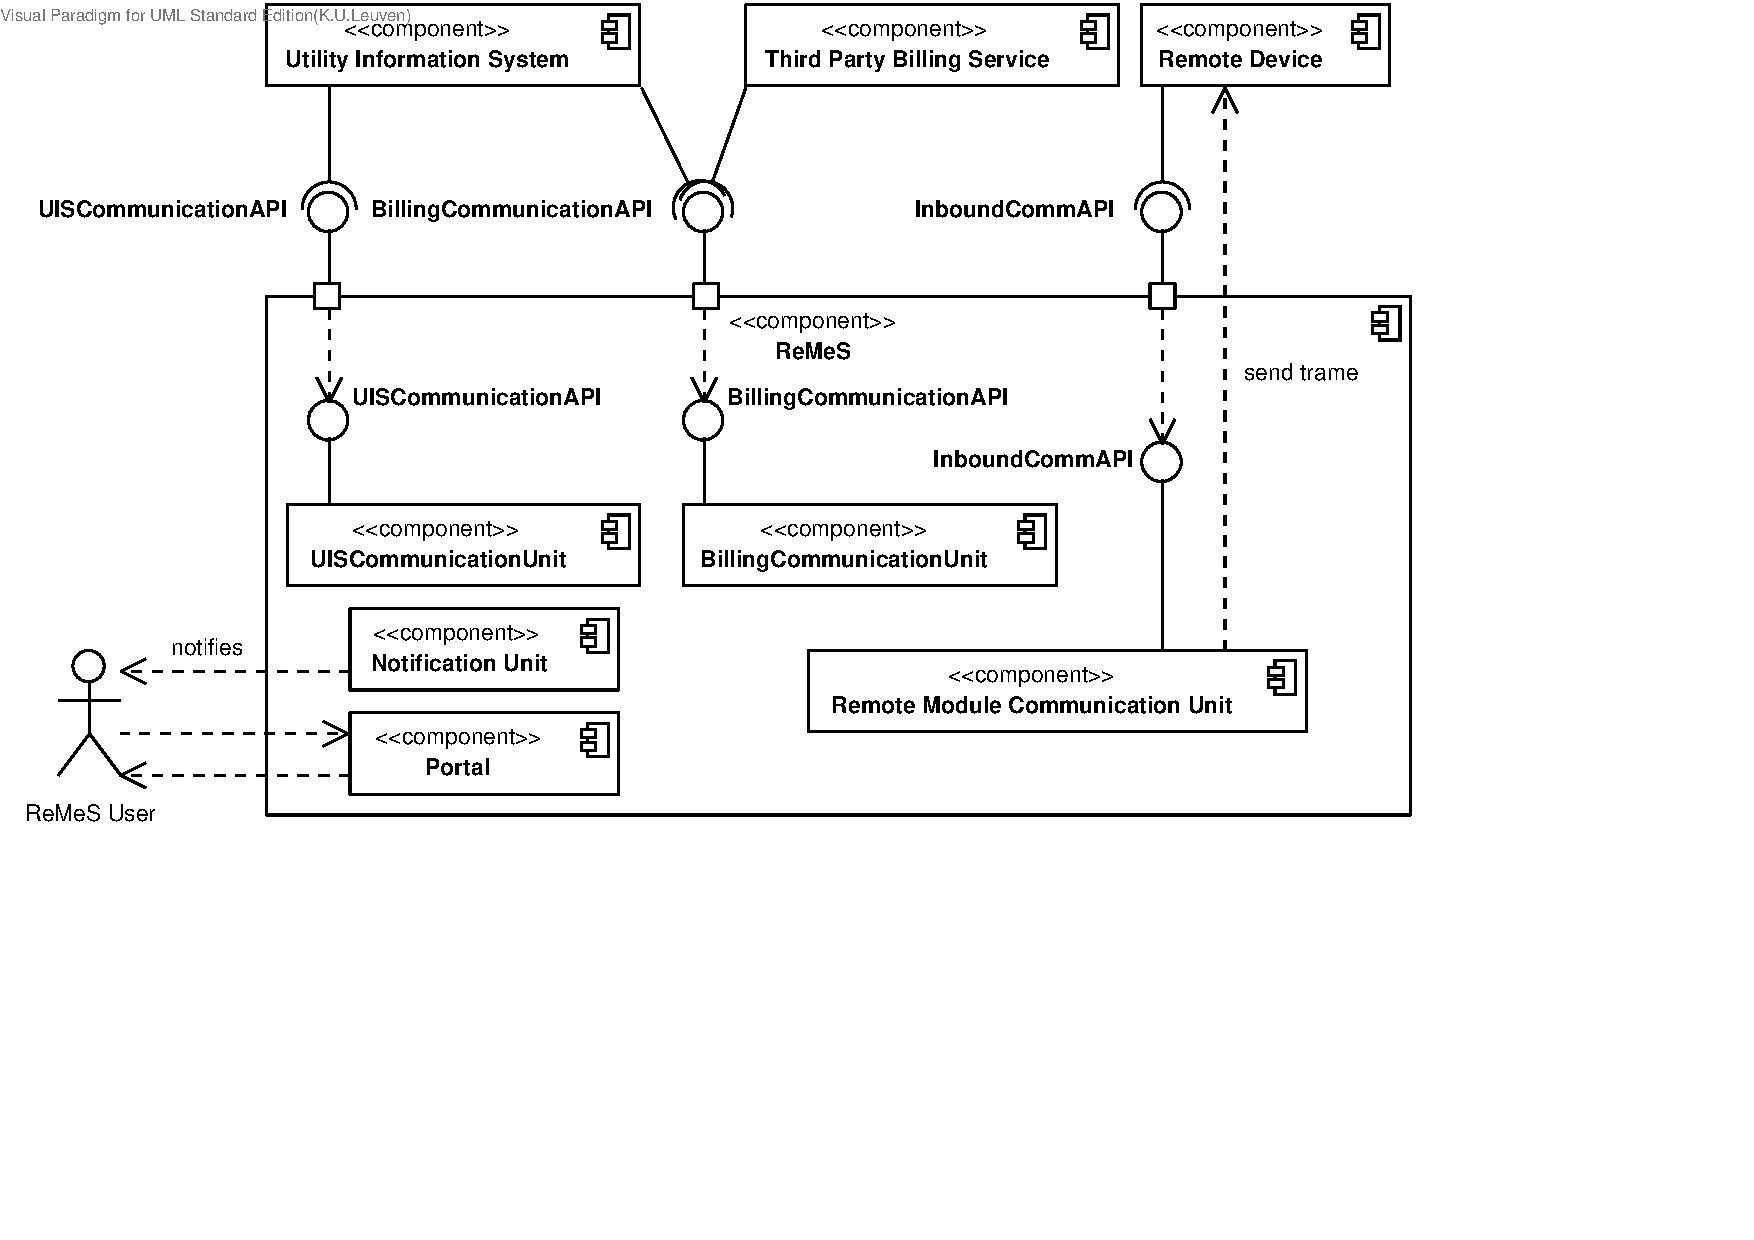
\includegraphics[width=\textwidth]{figs/final-context.pdf}
		\caption{The context diagram}
		\label{fig:final-context}
	\end{centering}
\end{figure}

\npar Figure \ref{fig:final-context} shows the context diagram. The ReMeS
user is a generalisation for all actors who can interact with the portal. 

\section{Overall Component Diagram}

\begin{figure}
	\begin{centering}
		% TODO Figure
		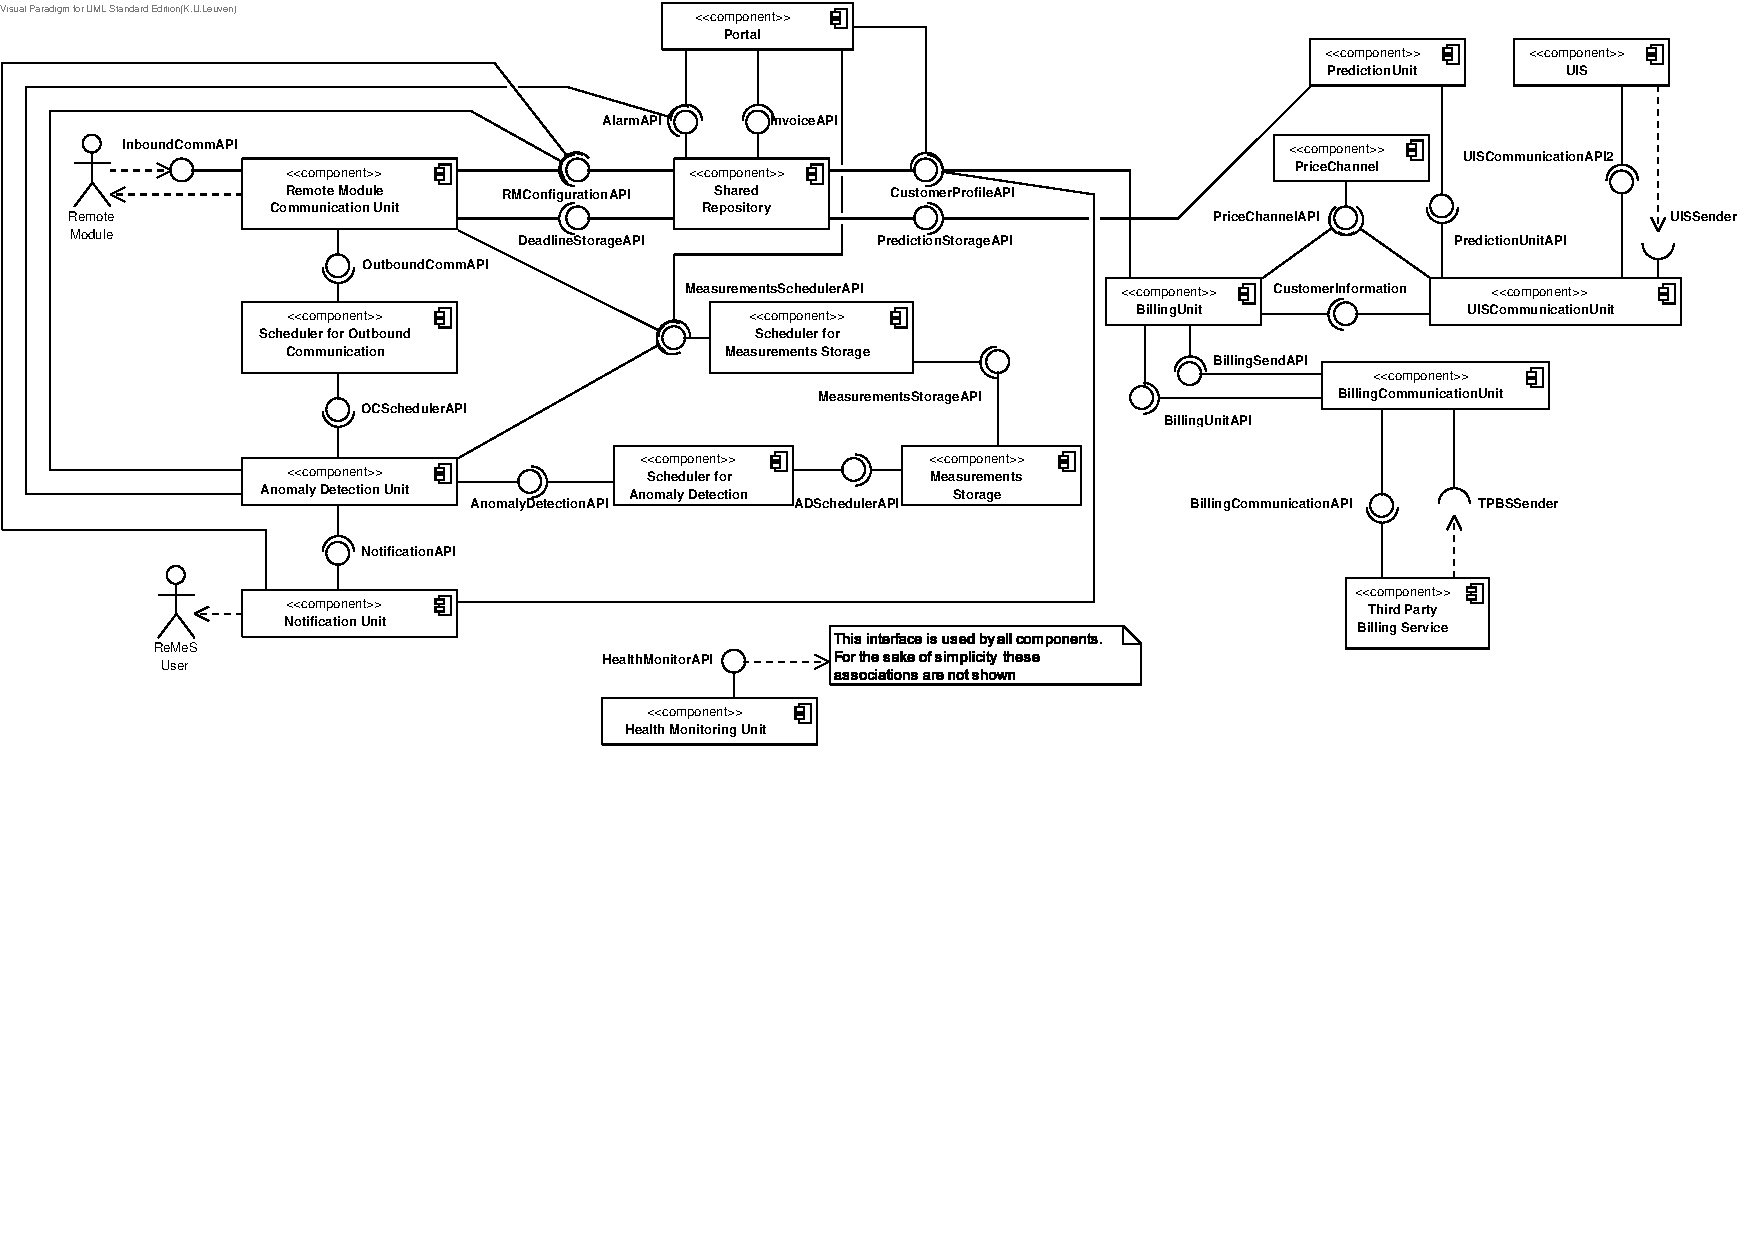
\includegraphics[height=\textwidth,angle=90]{figs/final-component.pdf}
		\caption{The component diagram of the overall system}
		\label{fig:final-components}
	\end{centering}
\end{figure}

\section{Key Decompositions}

\npar In this section there will be a short overview of all iterations of the
ADD process, recapitulating every iteration by its corresponding interface
diagram. In every subsection there will be a link to the ADD chapter where to
find detailed information explaining all components and interfaces of the
diagram.

\subsection{Whole system}

\npar In diagram \ref{fig:final-architecture/it1} all the components of the
first iteration are shown. The explanation for the roles and responsibilities
respectively interfaces can be found in sections \ref{add:it1/elements} and
\ref{add:it1/interfaces}.

\begin{figure}[H]
	\begin{centering}
		% TODO Figure
		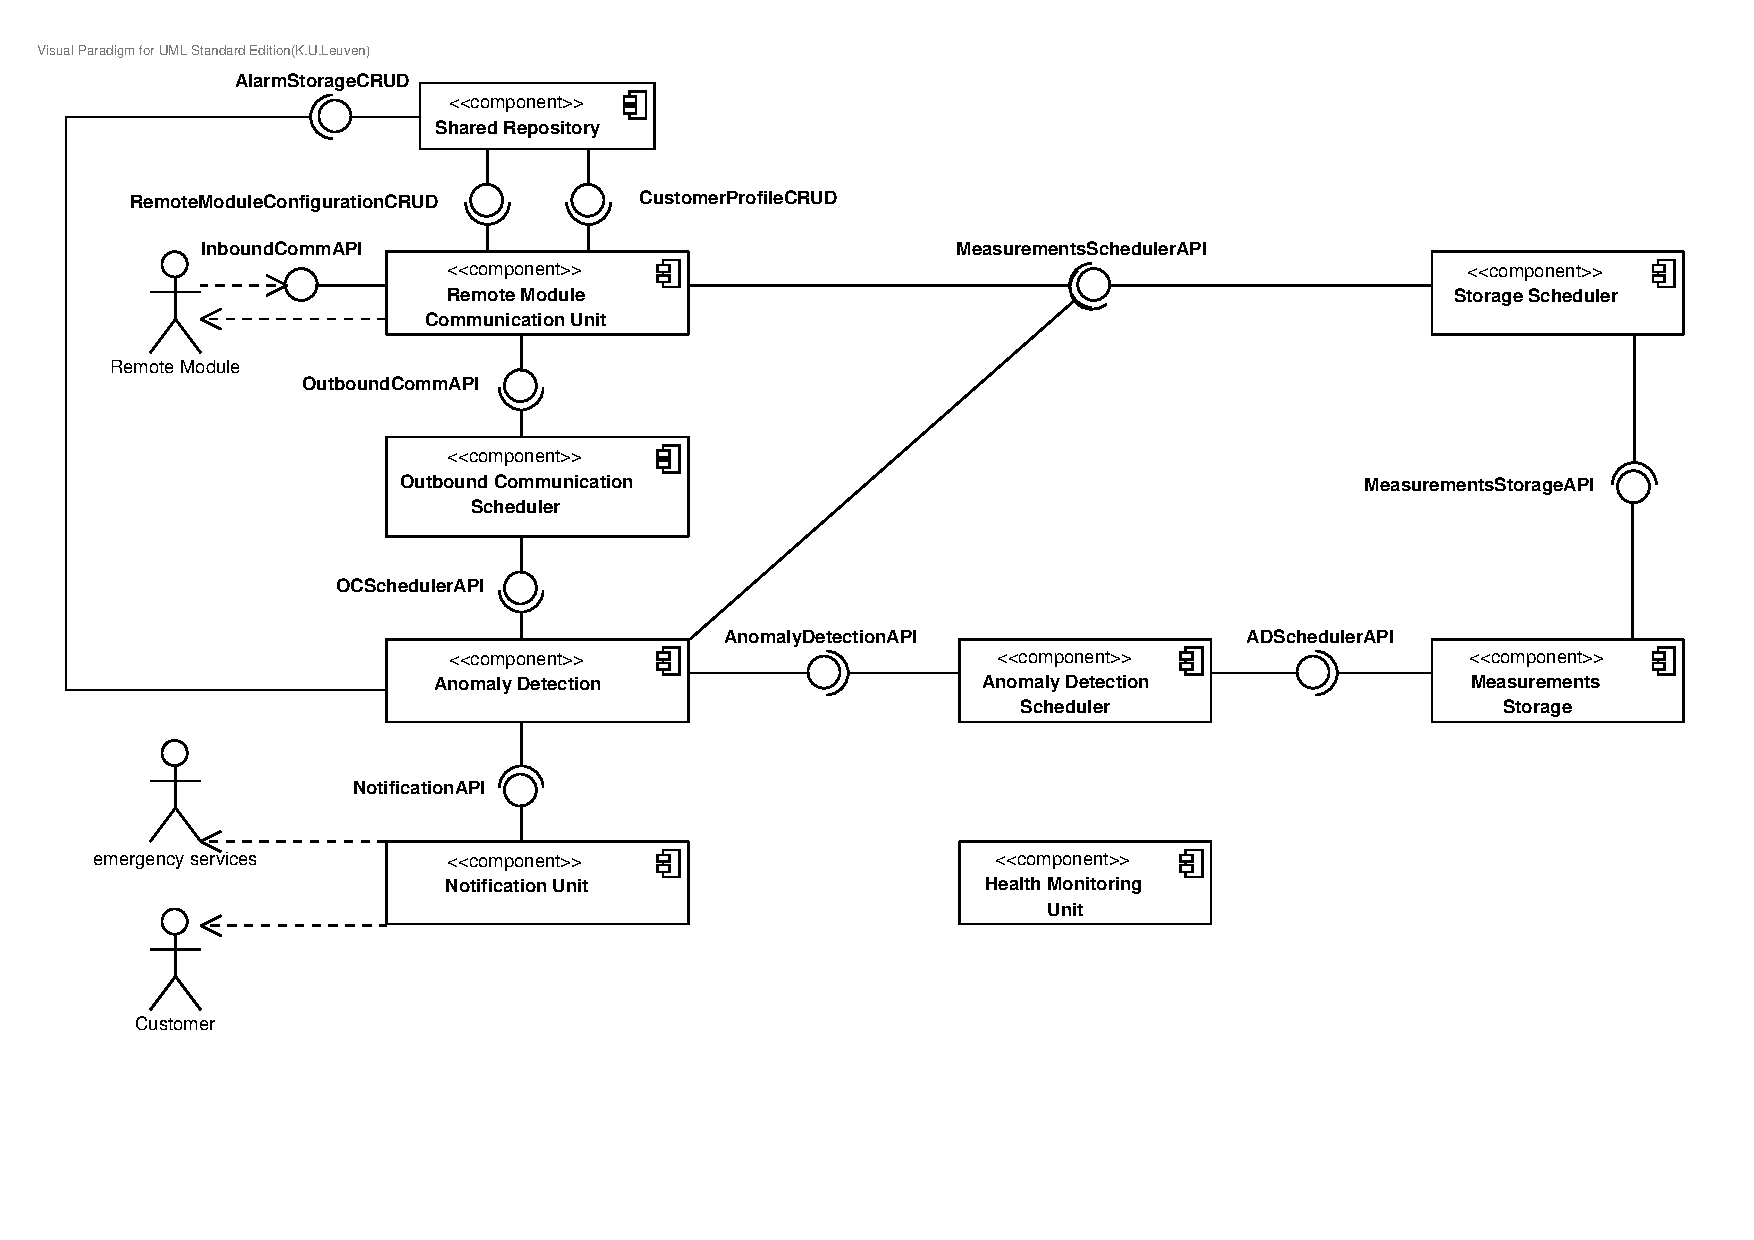
\includegraphics[height=\textwidth,angle=90]{figs/add-it1-interfaces.pdf}
		\caption{Overview of the interfaces and components in the ReMeS
		System.}
		\label{fig:final-architecture/it1}
	\end{centering}
\end{figure}

\subsection{Remote Module Communication Unit}

\npar The results of the second iteration are visualized in figure
\ref{fig:final-architecture/it2}. The corresponding components and interface
explanation can be found in respectively section \ref{add:it2/elements} and
\ref{add:it2/interfaces}.

\begin{figure}[H]
	\begin{centering}
		% TODO Figure
		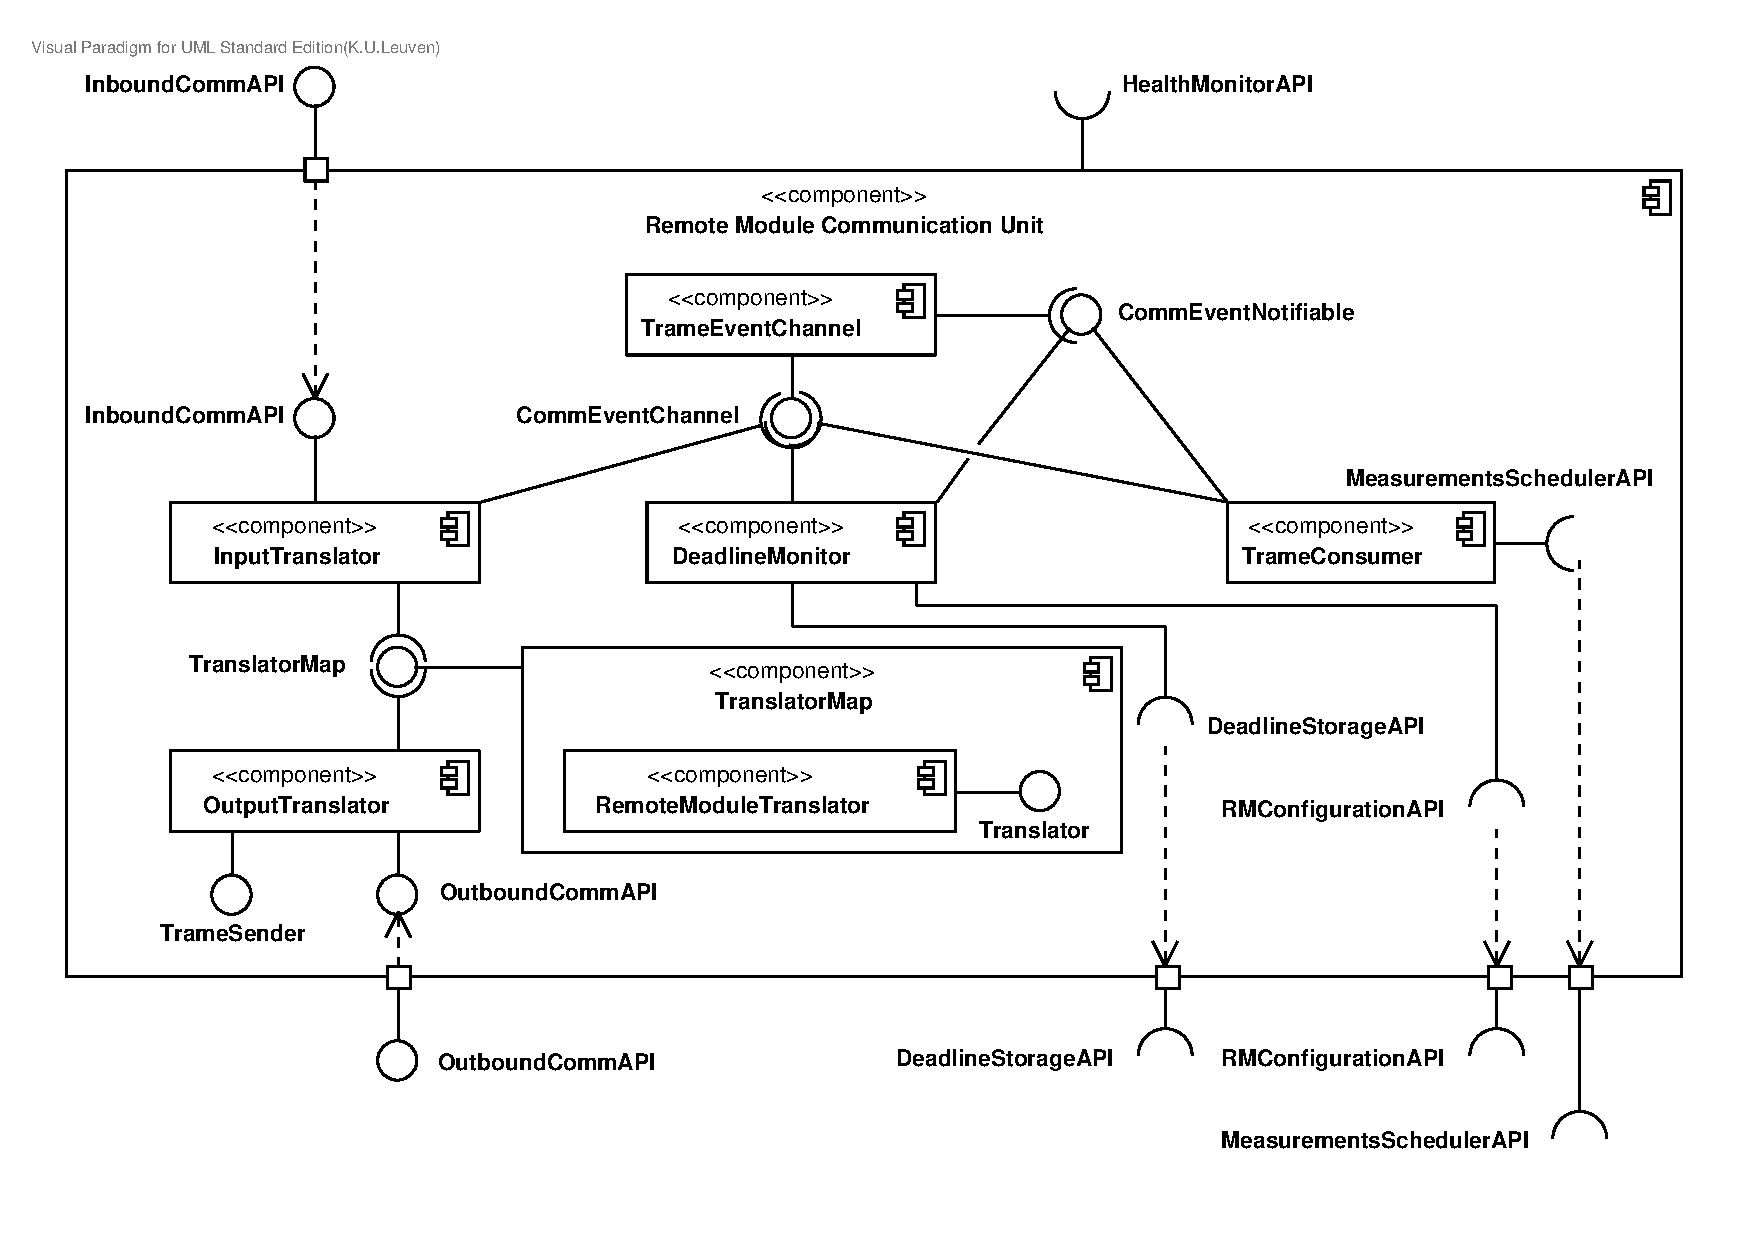
\includegraphics[width=\textwidth]{figs/add-it2-interfaces.pdf}
		\caption{Overview of the interfaces and components in the Remote
		Module Communication Unit.}
		\label{fig:final-architecture/it2}
	\end{centering}
\end{figure}

\subsection{Scheduler For MeasurementsStorage}

\npar Figure \ref{fig:final-architecture/it3} shows all the components of the
Scheduler for MeasurementsStorage, this was the third iteration. The roles and
responsibilties of each component can be found in \ref{add:it3/elements}. The
interfaces documentation is stated in section \ref{add:it3/interfaces}.

\begin{figure}[H]
	\begin{centering}
		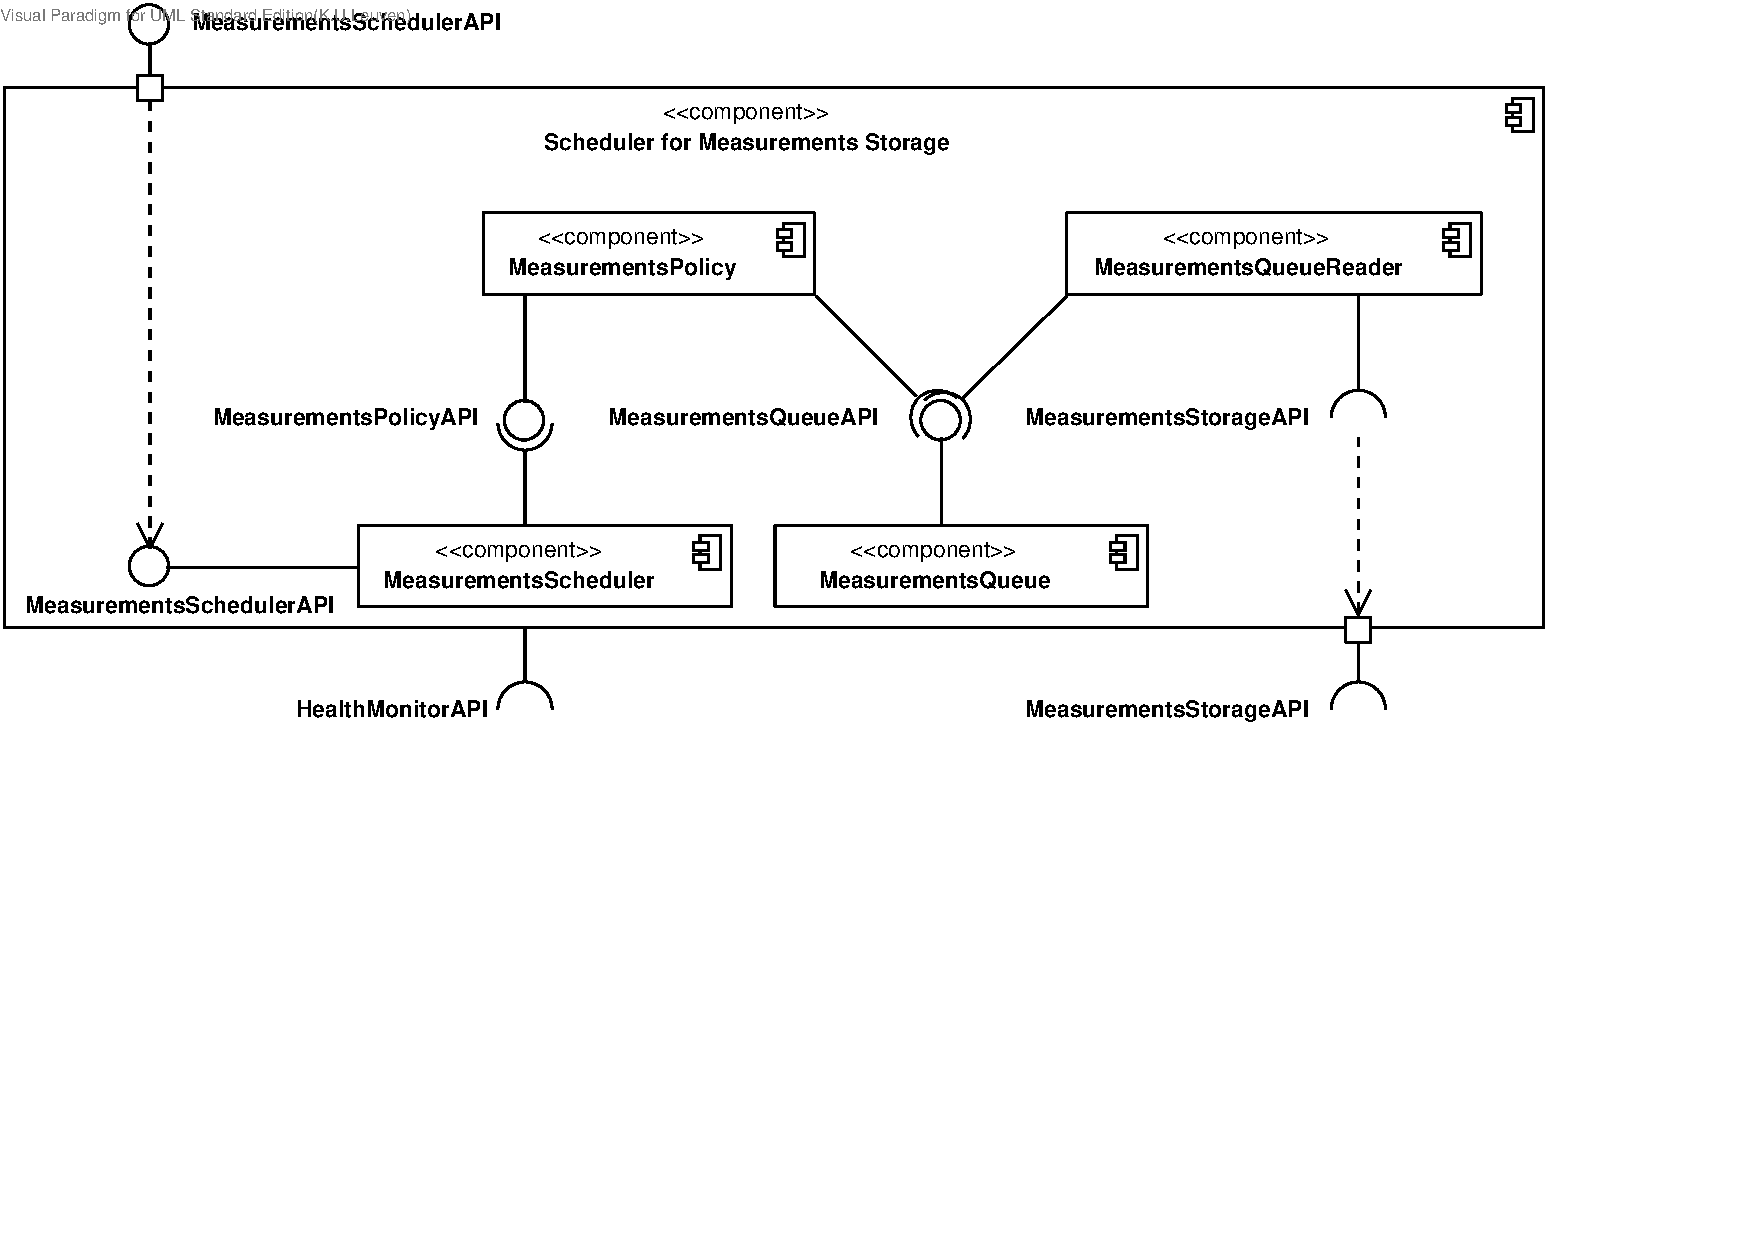
\includegraphics[width=\textwidth]{figs/add-it3-interfaces.pdf}
		\caption{Overview of the interfaces and components in the Scheduler For
		MeasurementsStorage.}
		\label{fig:final-architecture/it3}
	\end{centering}
\end{figure}

\subsection{MeasurementsStorage}

\npar The results of the fourth iteration are visible in figure
\ref{fig:final-architecture/it4}. Interface documentation can be found in
section \ref{add:it4/interfaces}. The component explanation is documented in
section \ref{add:it4/elements}.

\begin{figure}[H]
	\begin{centering}
		% TODO Figure
		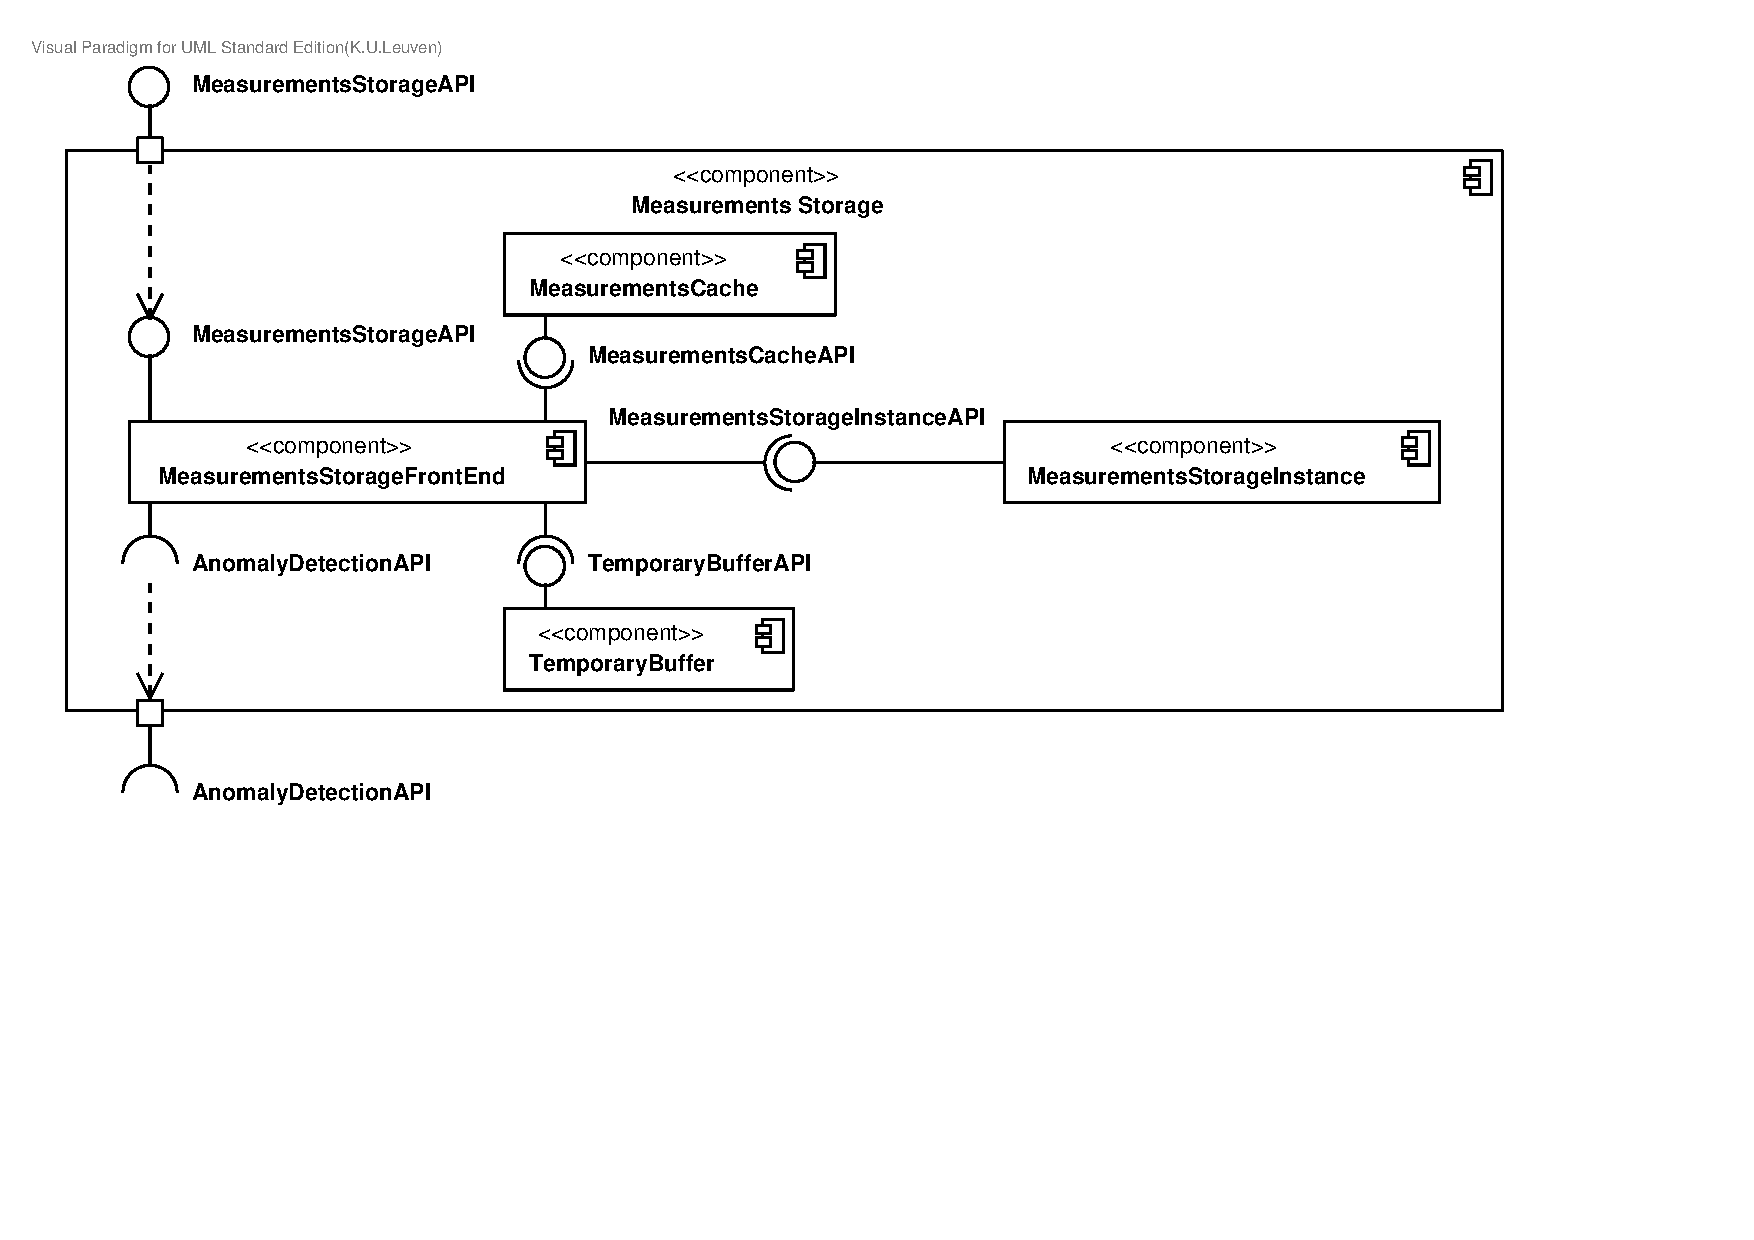
\includegraphics[width=\textwidth]{figs/add-it4-interfaces.pdf}
		\caption{Overview of the interfaces and components in the
		MeasurementsStorage.}
		\label{fig:final-architecture/it4}
	\end{centering}
\end{figure}

\subsection{Scheduler For Anomaly Detection}

\npar Iteration 5 discussed the decomposition of the scheduler for anomaly
detection. The results are shown in figure \ref{fig:final-architecture/it5}. The
component and interface documentation can be found in respectively section
\ref{add:it5/elements} and \ref{add:it5/interfaces}.

\begin{figure}[H]
	\begin{centering}
		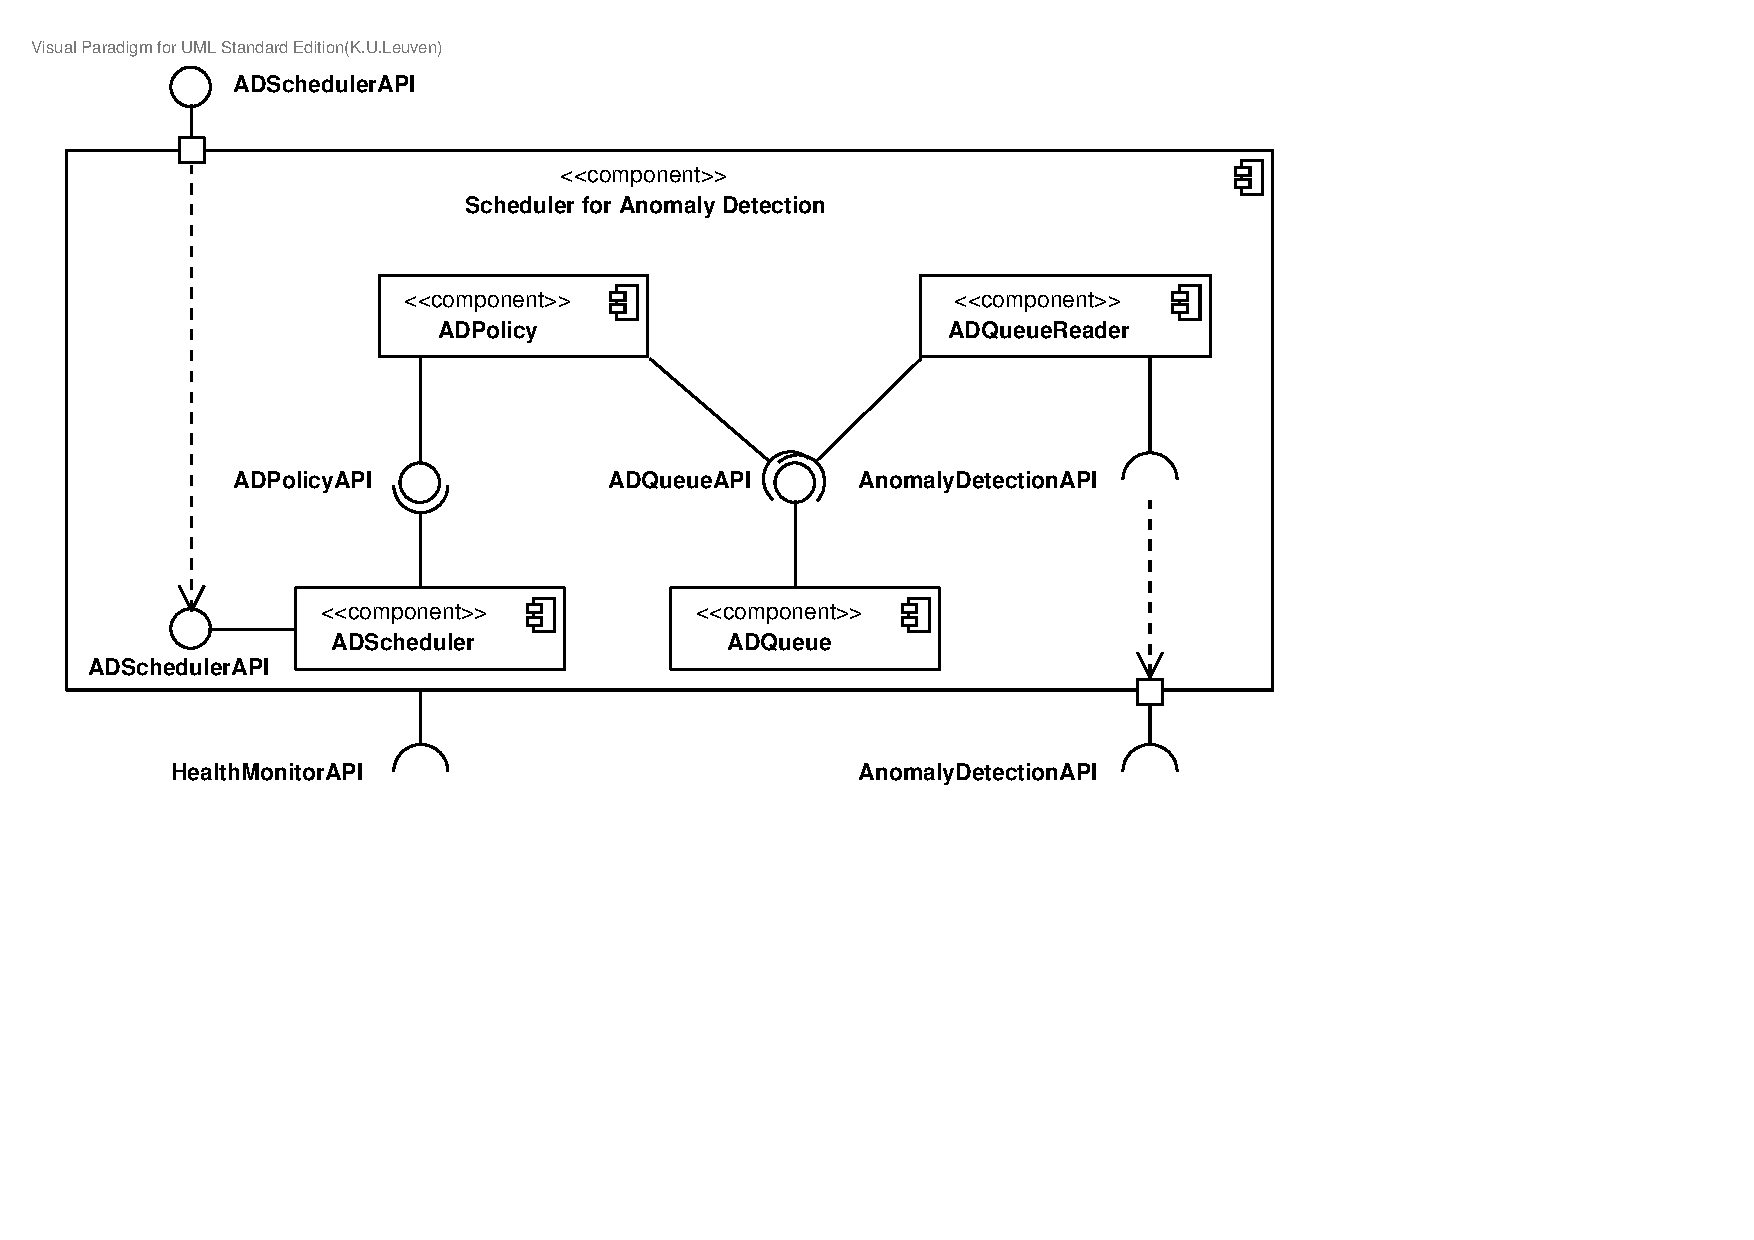
\includegraphics[width=\textwidth]{figs/add-it5-interfaces.pdf}
		\caption{Overview of the interfaces and components in the Scheduler For
		Anomaly Detection.}
		\label{fig:final-architecture/it5}
	\end{centering}
\end{figure}

\subsection{Anomaly Detection Unit}

\npar In figure \ref{fig:final-architecture/it6} is the decomposition of the
Anomaly Detection Unit depicted. The explanation for the roles and
responsibilities of each component can be found in section
\ref{add:it6/elements}. The interface documentation is stated in section
\ref{add:it6/interfaces}.

\begin{figure}[H]
	\begin{centering}
		% TODO Figure
		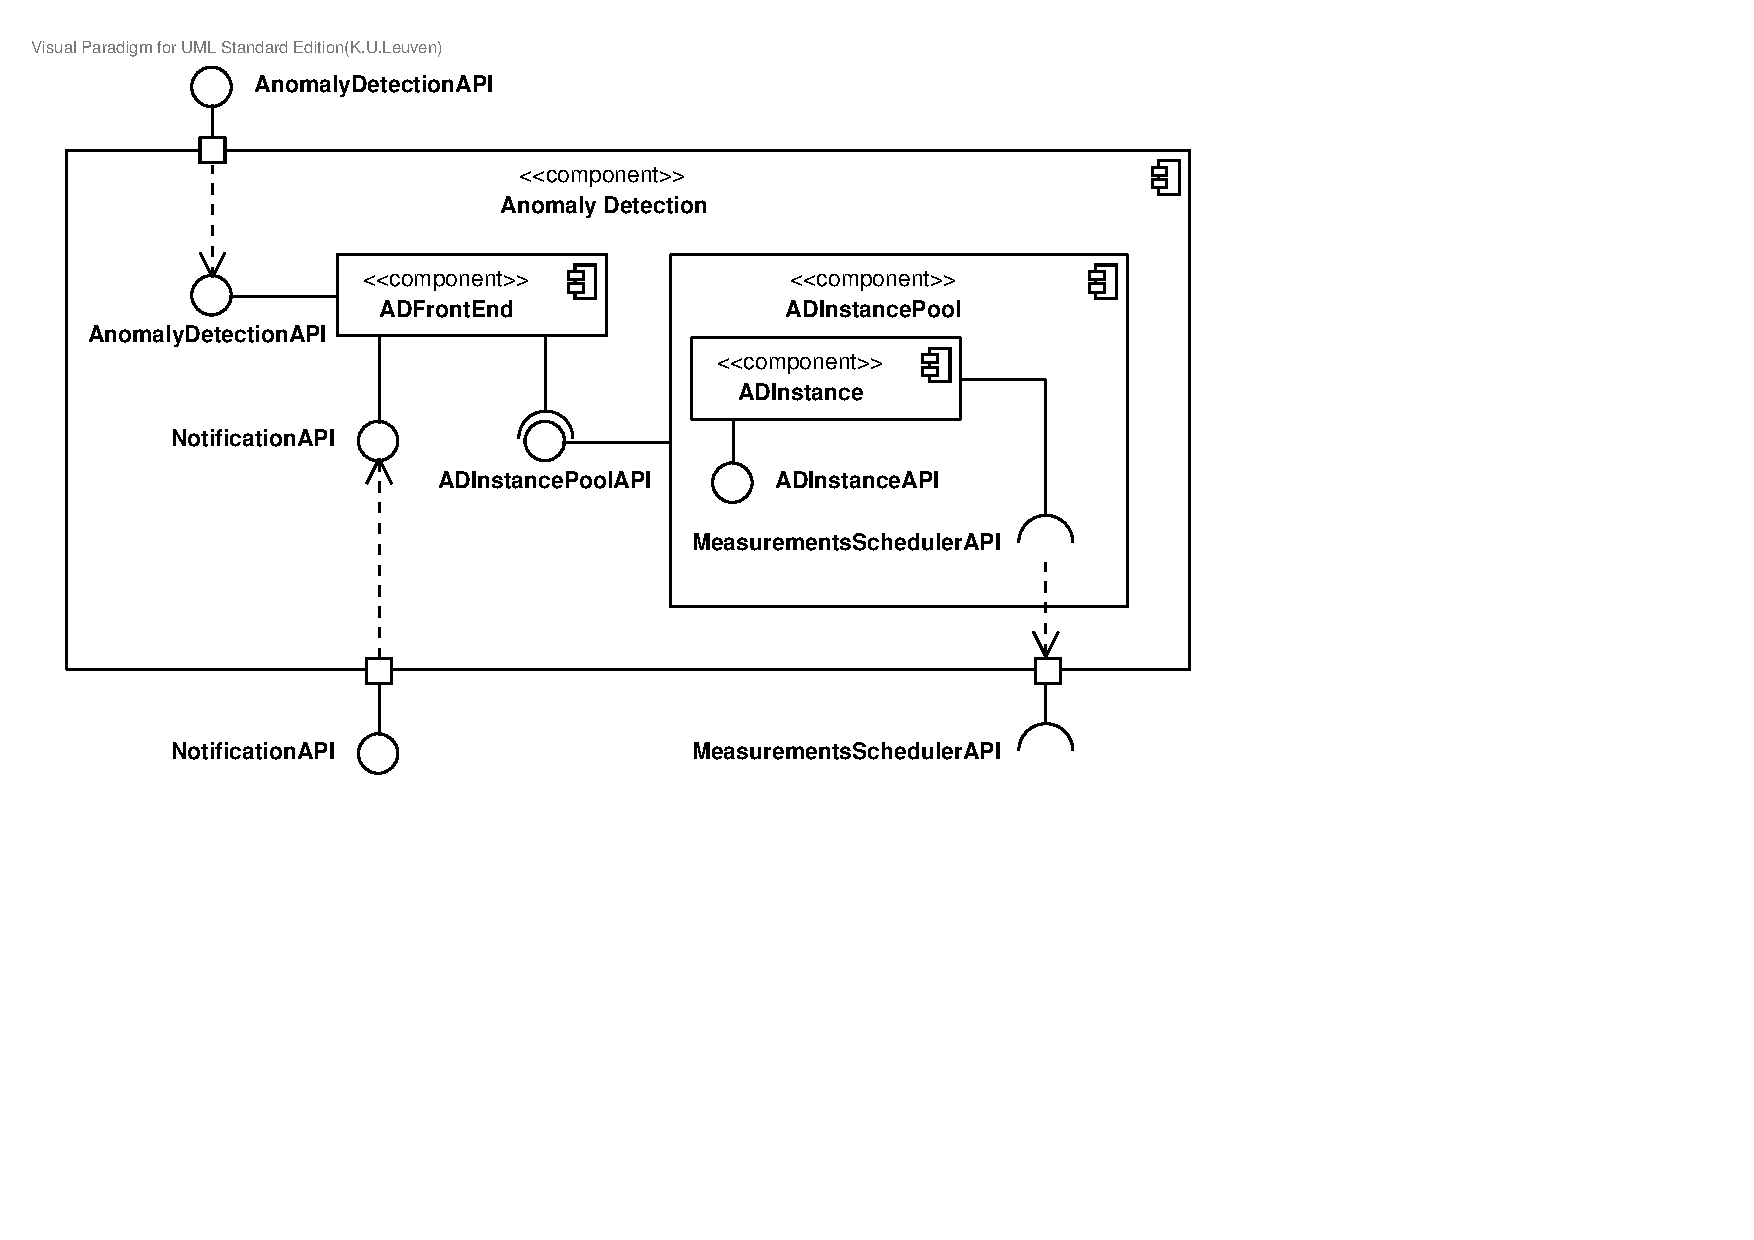
\includegraphics[width=\textwidth]{figs/add-it6-interfaces.pdf}
		\caption{Overview of the interfaces and components in the Anomaly Detection
		Unit.}
		\label{fig:final-architecture/it6}
	\end{centering}
\end{figure}

\subsection{Scheduler For Outbound Communication}

\npar The results of the seventh iteration are visualized in figure
\ref{fig:final-architecture/it7}. The corresponding components and interface
explanation can be found in respectively section \ref{add:it7/elements} and
\ref{add:it7/interfaces}.

\begin{figure}[H]
	\begin{centering}
		% TODO Figure
		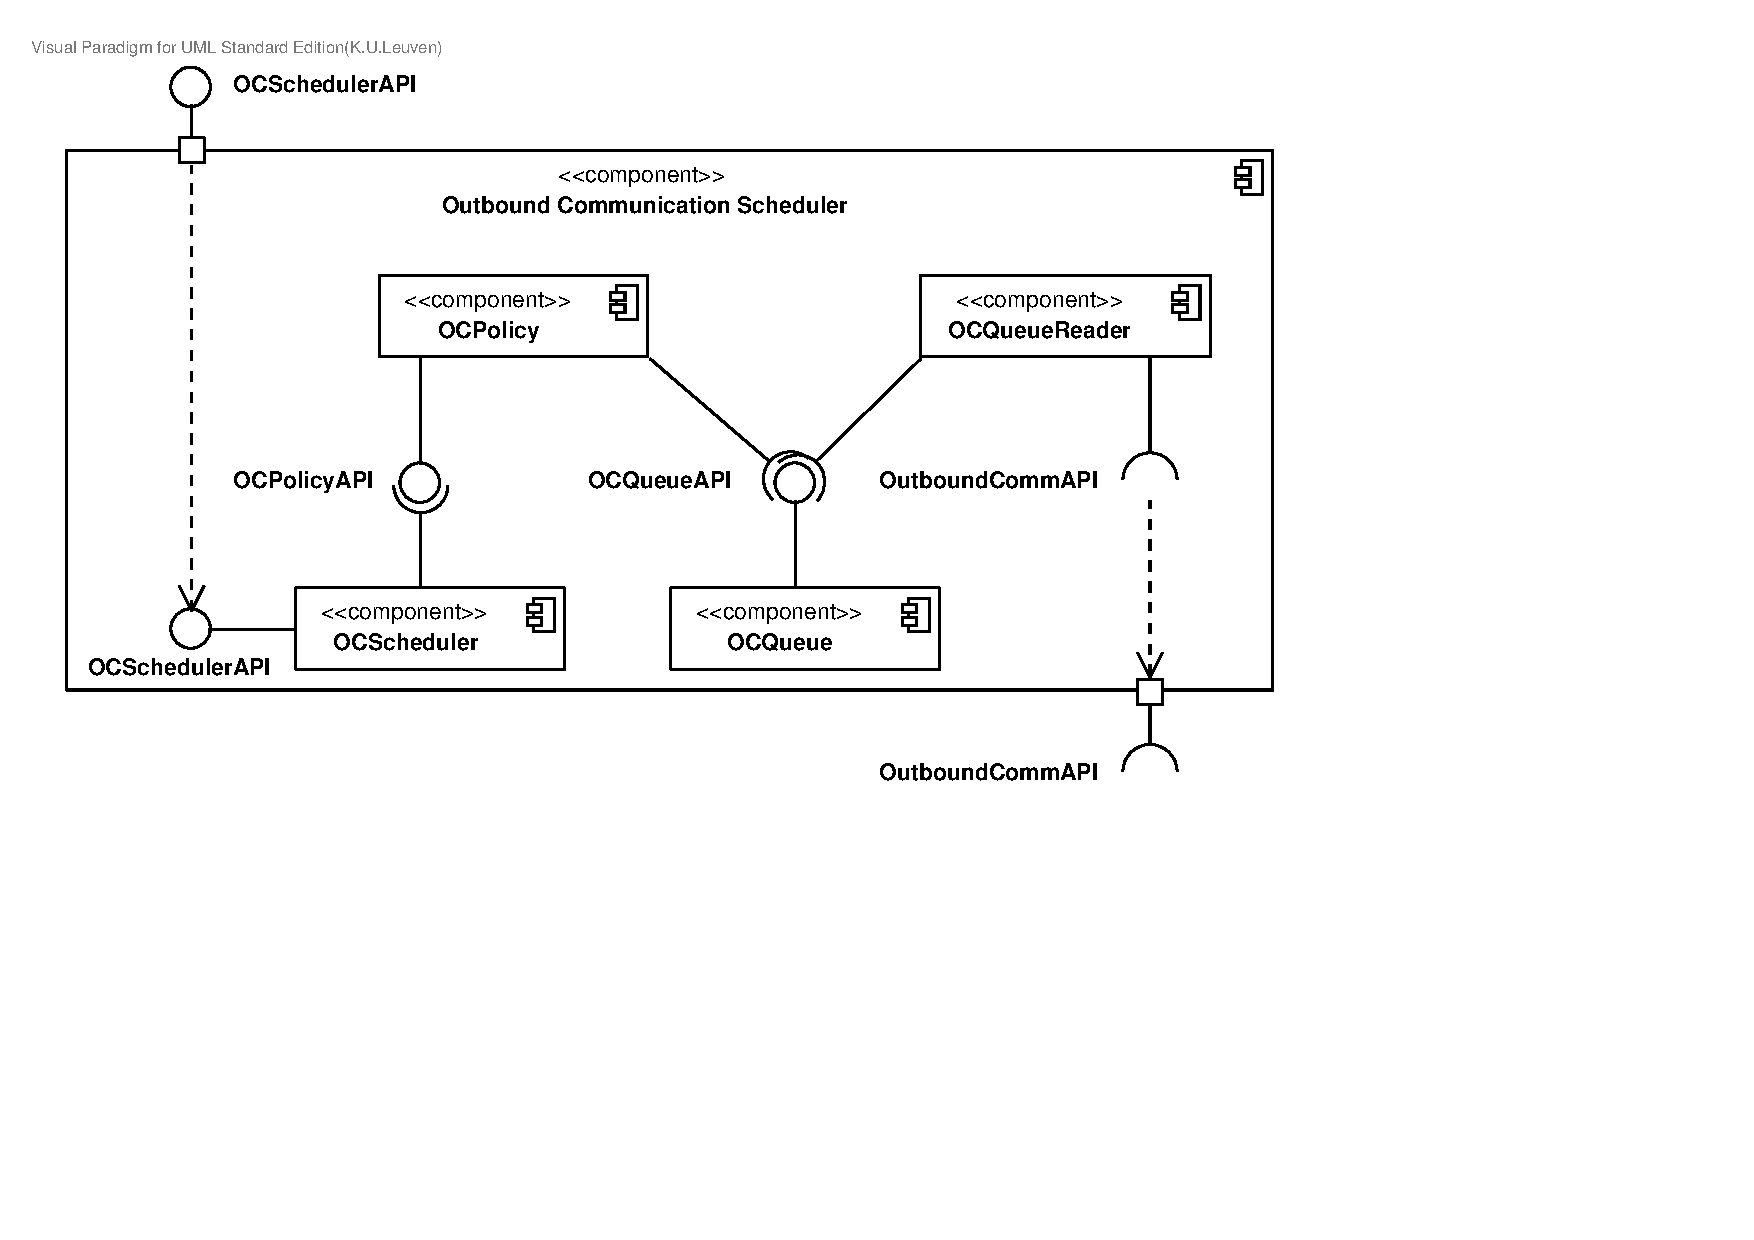
\includegraphics[width=\textwidth]{figs/add-it7-interfaces.pdf}
		\caption{Overview of the interfaces and components in the Scheduler For
		Outbound Communication.}
		\label{fig:final-architecture/it7}
	\end{centering}
\end{figure}

\subsection{Notification Unit}

\npar Figure \ref{fig:final-architecture/it8} depicts the decomposition of the
Notification Unit. A detailed explanation of each component can be found in
\ref{add:it8/elements}. The interface documentation is to be found in section
\ref{add:it8/interfaces}.

\begin{figure}[H]
	\begin{centering}
		% TODO Figure
		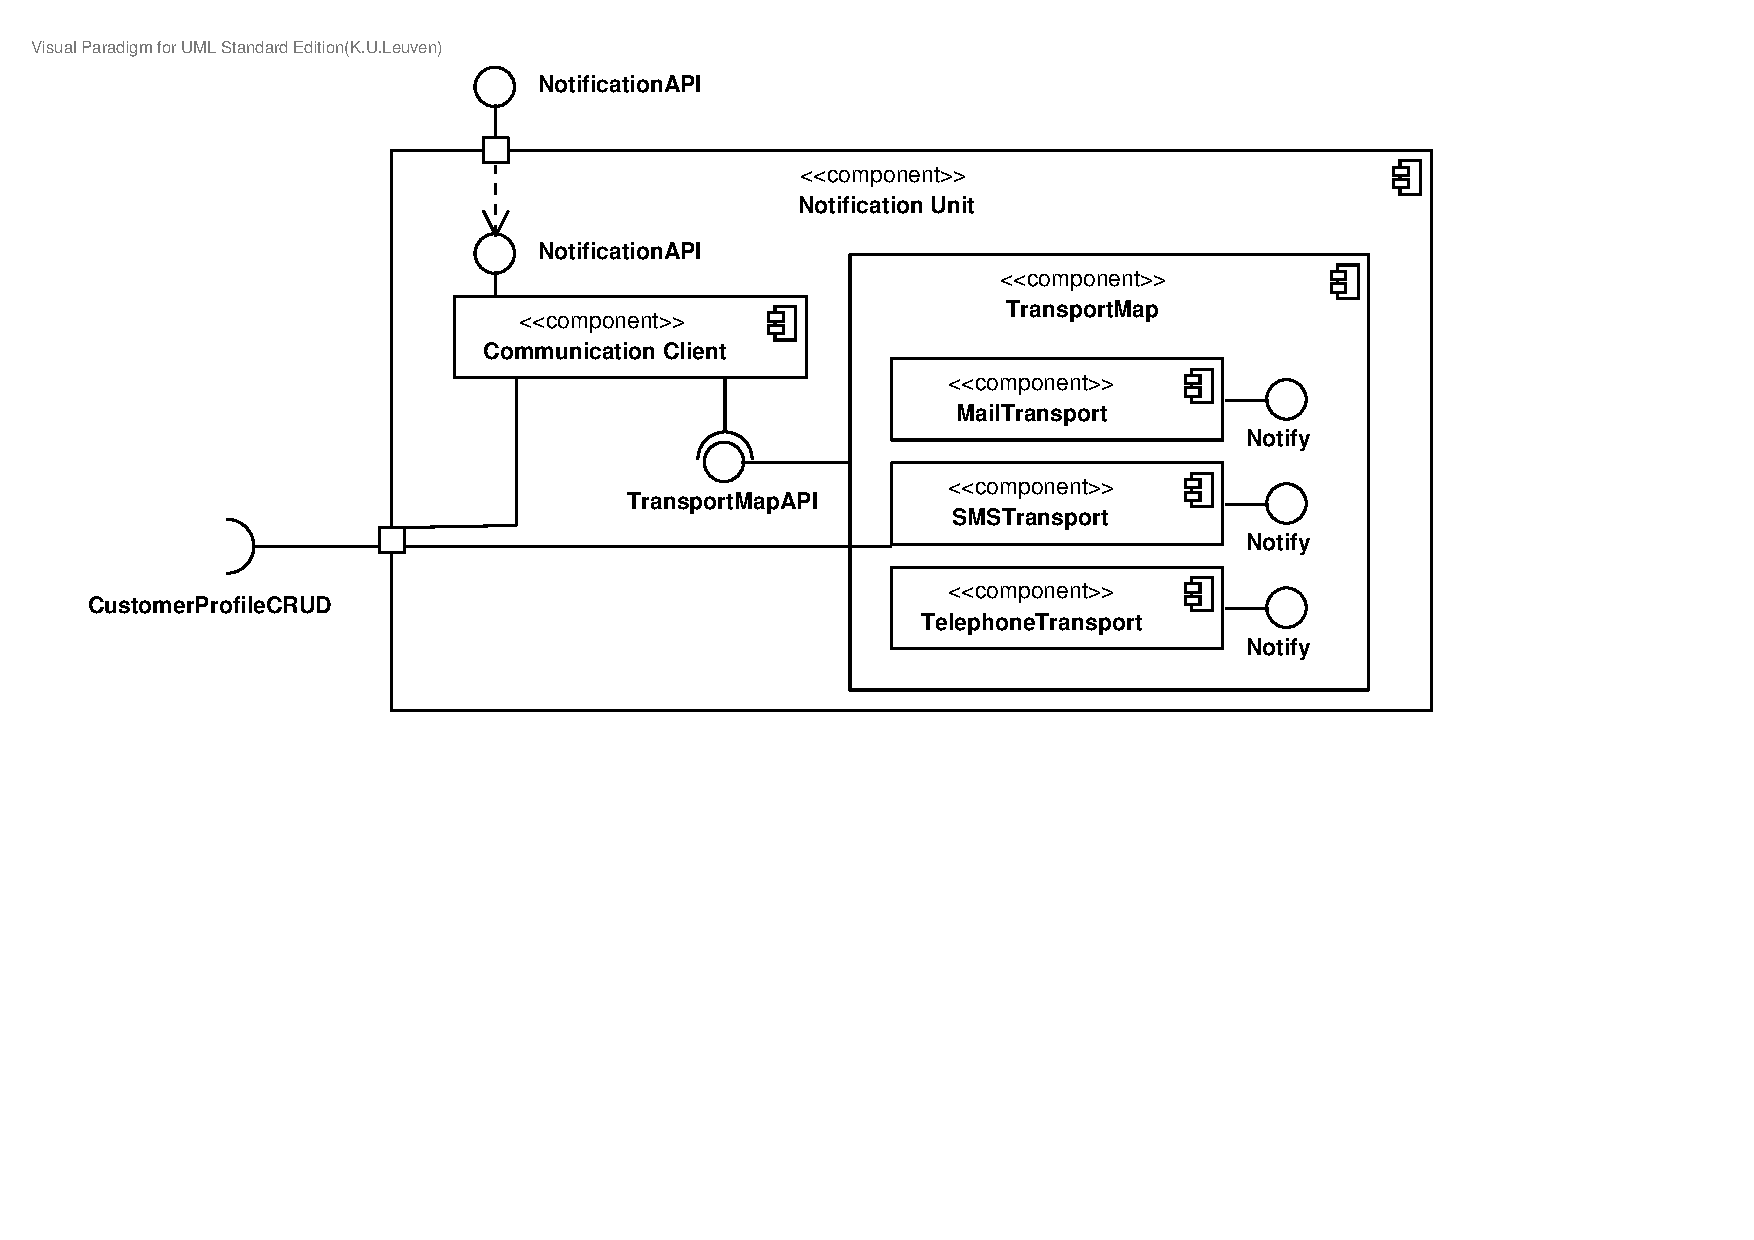
\includegraphics[width=\textwidth]{figs/add-it8-interfaces.pdf}
		\caption{Overview of the interfaces and components in the Notification Unit.}
		\label{fig:final-architecture/it8}
	\end{centering}
\end{figure}

\subsection{Health Monitoring Unit}

\npar Iteration 5 discussed the decomposition of the Health Monitoring Unit. The
results are shown in figure \ref{fig:final-architecture/it9}. The component and
interface documentation can be found in respectively section
\ref{add:it9/elements} and \ref{add:it9/interfaces}.

\begin{figure}[H]
	\begin{centering}
		% TODO Figure
		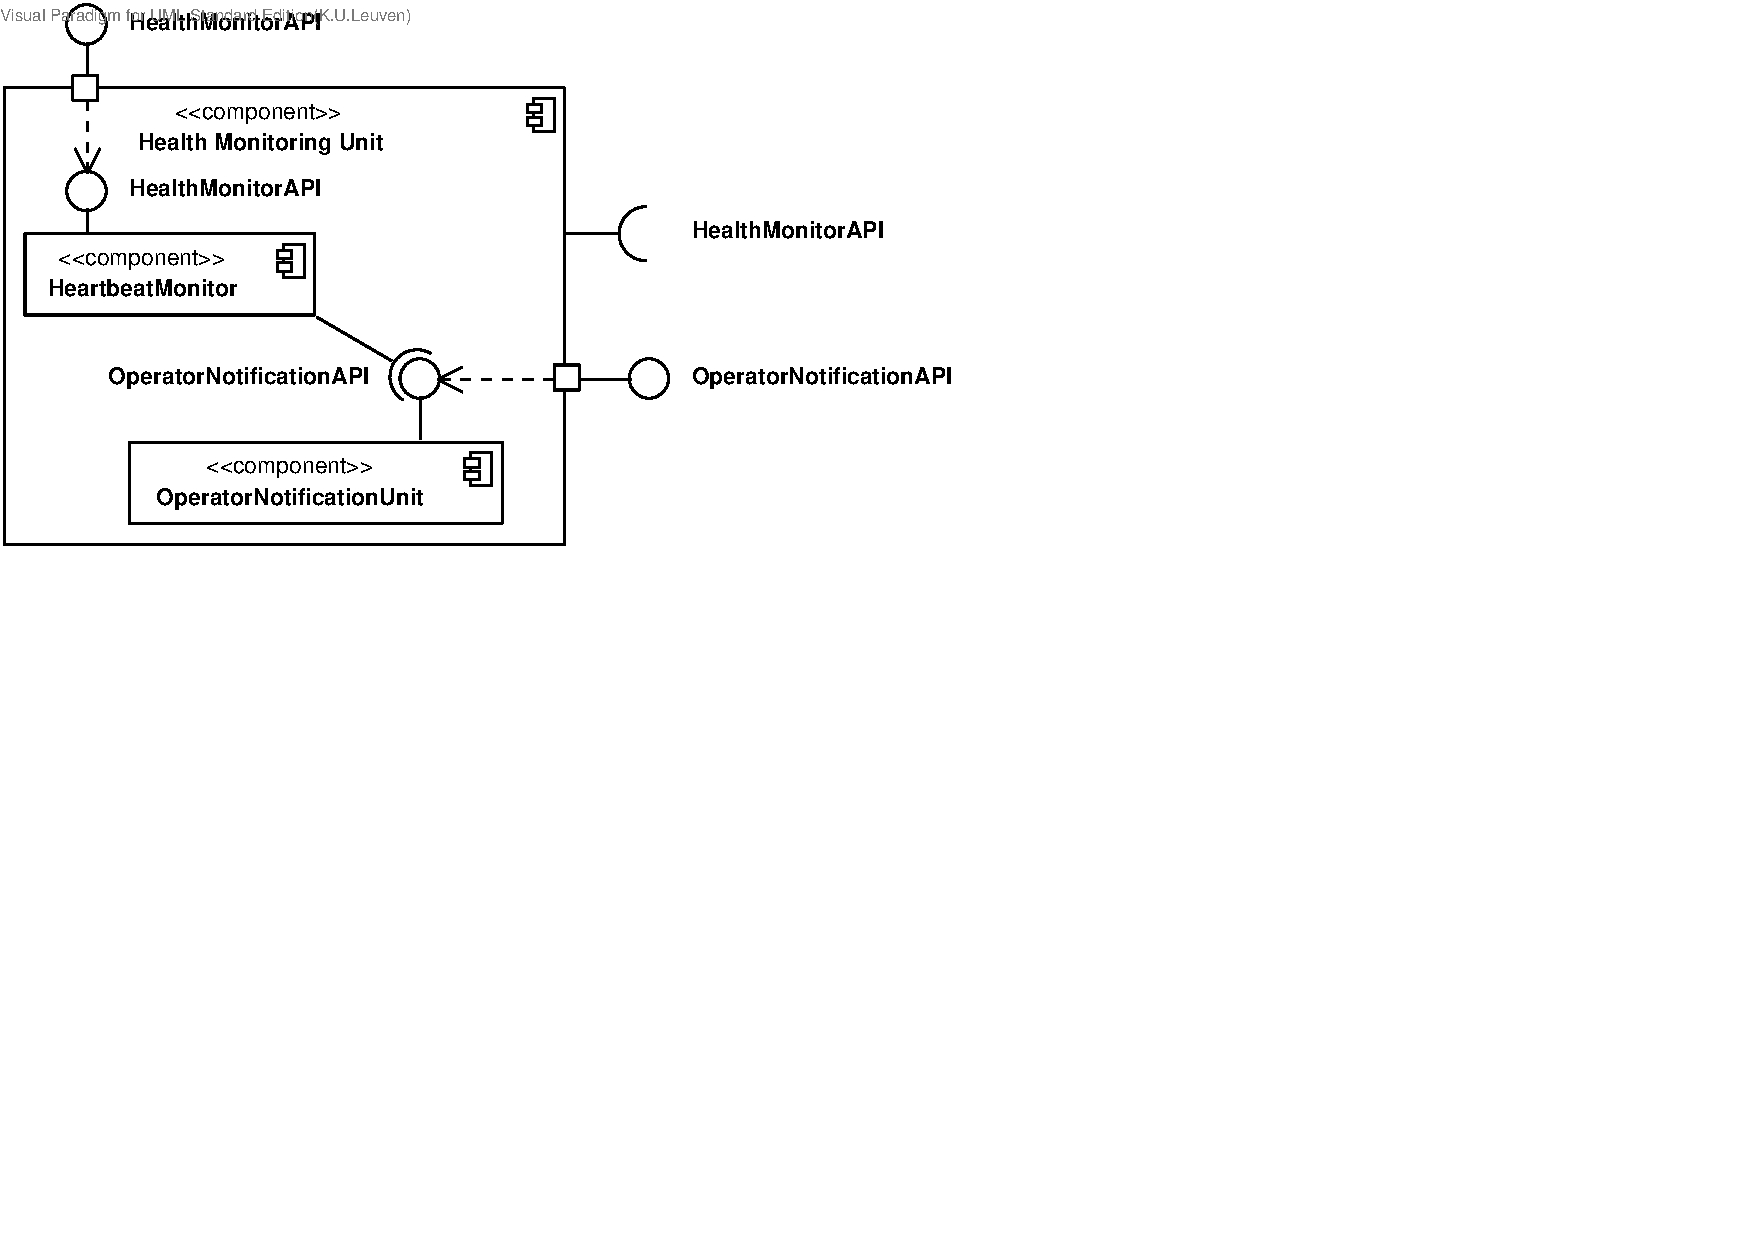
\includegraphics[width=\textwidth]{figs/add-it9-interfaces.pdf}
		\caption{Overview of the interfaces and components in the Health Monitoring
		Unit.}
		\label{fig:final-architecture/it9}
	\end{centering}
\end{figure}

\subsection{Other}

\npar The final iteration, the tenth, contains the decomposition of the other
component. It is very important to remark that there never will be any notion of
an ``other component'' in the system once one starts implementing it. This can
also be seen in the overall component diagram, see \ref{fig:final-components}.
Nonetheless is it shown in diagram \ref{fig:final-architecture/it10}, but it has
no functional meaning except for grouping the components. Documentation of the
components can be found in section \ref{add:it10/elements}. The interface
explanation is to be found in section \ref{add:it10/interfaces}.

\begin{figure}[H]
	\begin{centering}
		% TODO Figure 
		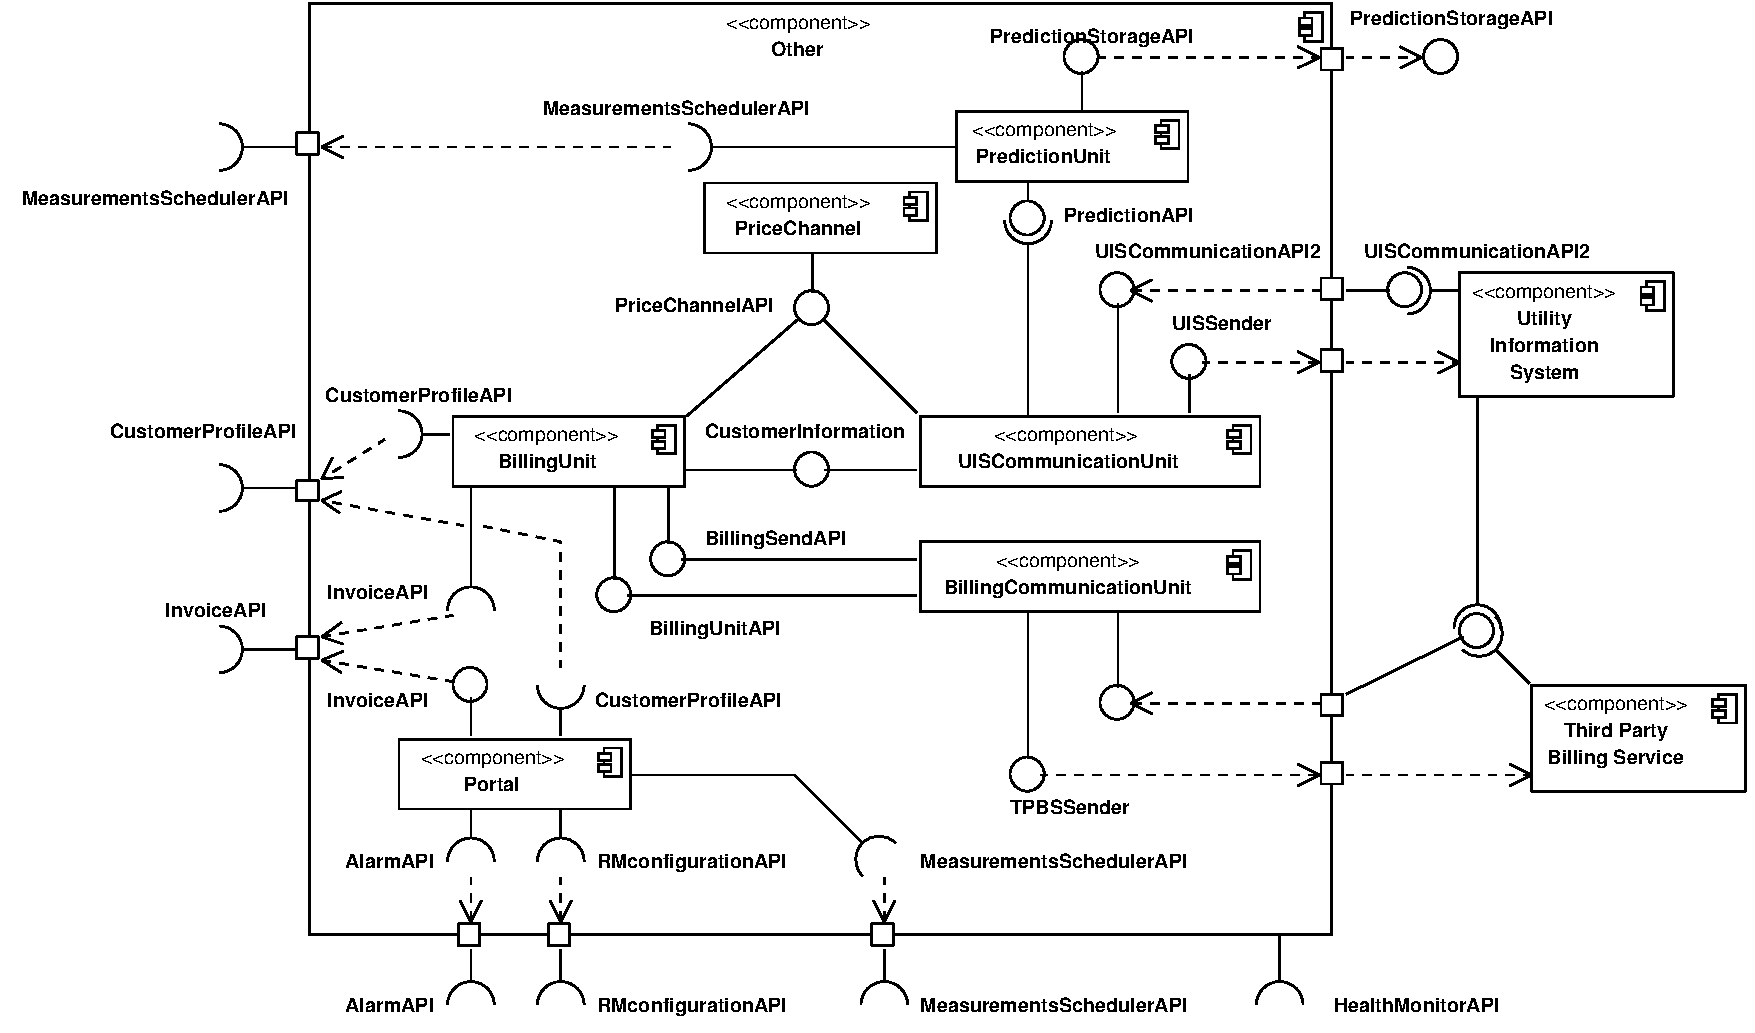
\includegraphics[width=\textwidth]{figs/add-it10-interfaces.pdf}
		\caption{Overview of the interfaces and components in the Other component.}
		\label{fig:final-architecture/it10}
	\end{centering}
\end{figure}

\section{Deployment Diagram}

\npar The deployment diagram is shown in figure \ref{fig:final-deployment}. 

\begin{figure}
	\begin{centering}
		% TODO Figure
		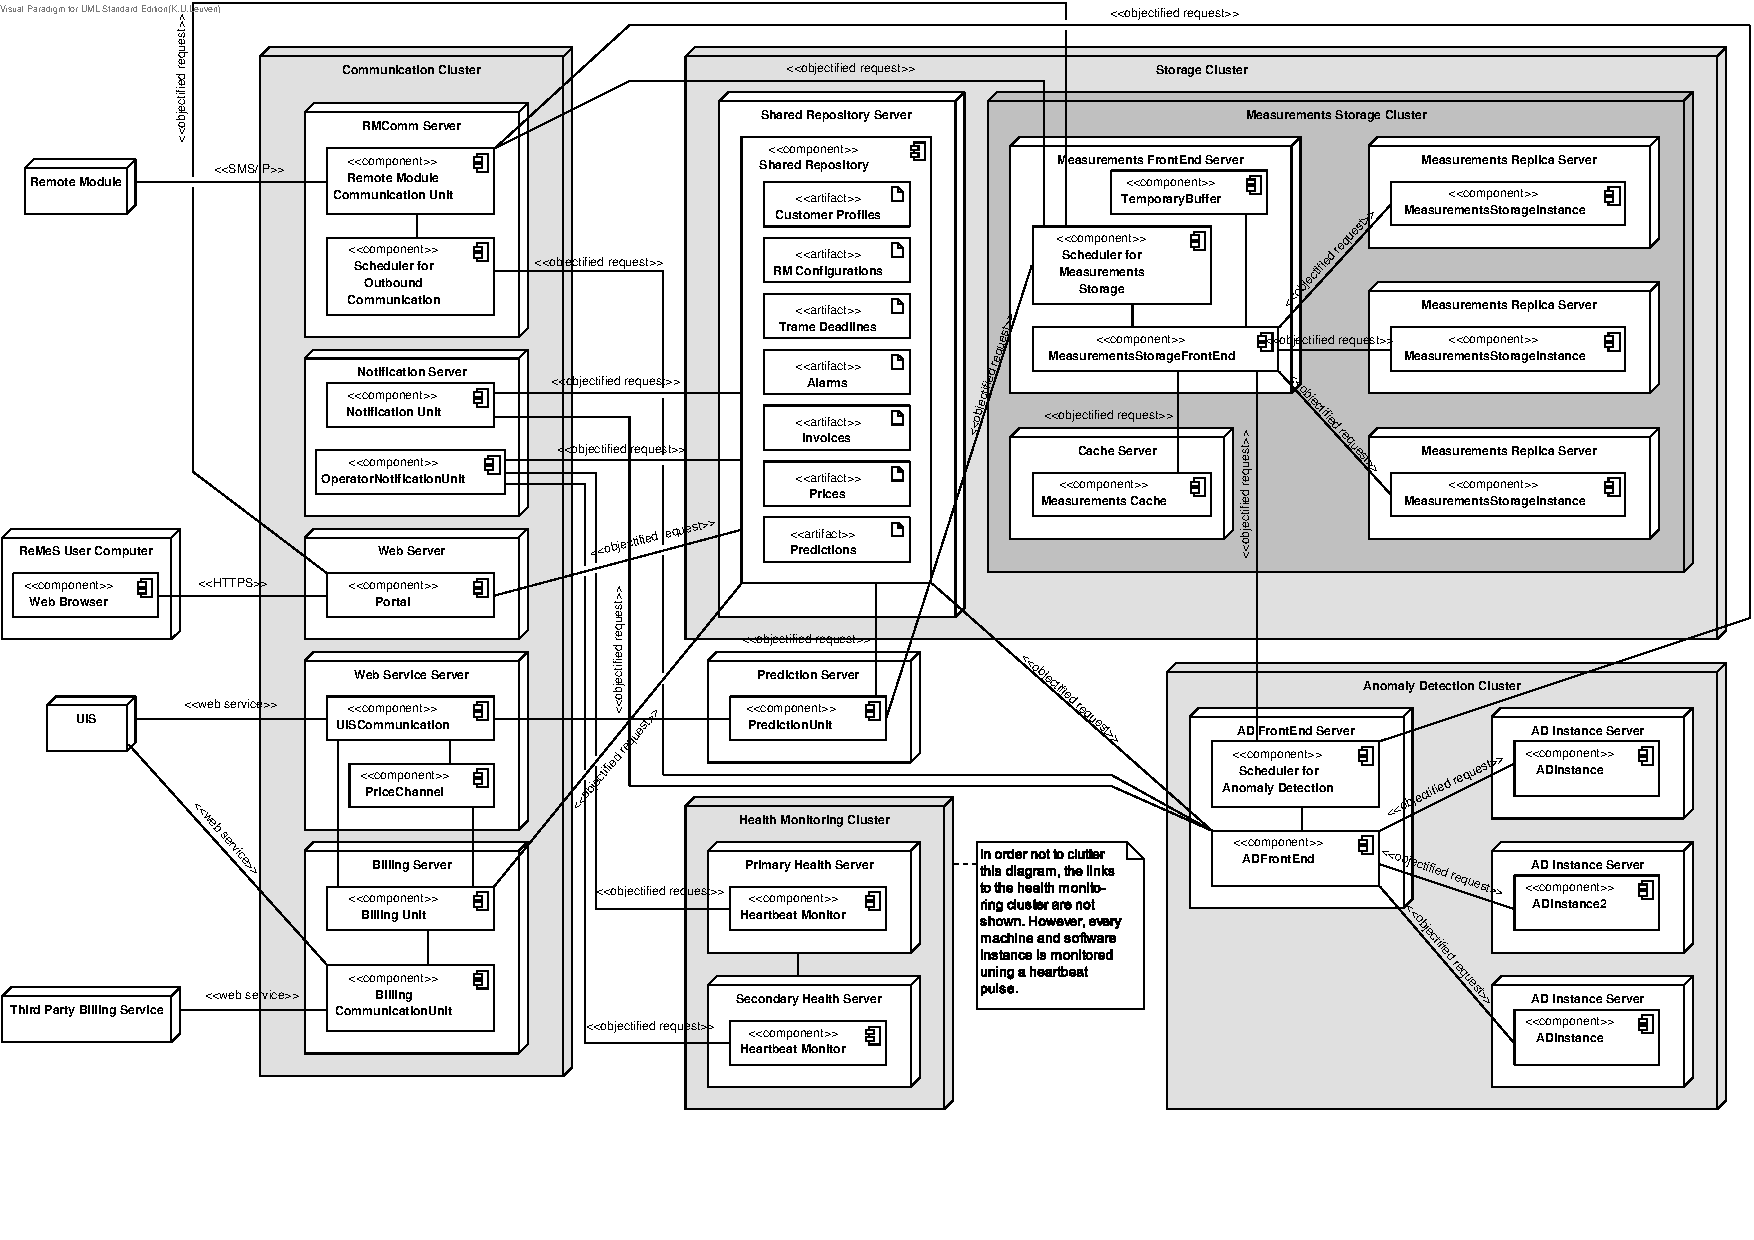
\includegraphics[height=\textwidth,angle=90]{figs/final-deployment.pdf}
		\caption{The deployment diagram}
		\label{fig:final-deployment}
	\end{centering}
\end{figure}

\npar A trame always arrives at the RMComm Server in the Communication Cluster.
This server acts as a gateway for all remote module communication. It will also
host the scheduler for outbound communication. To summarize, the RMComm Server
is responsible for all trame communication. 

\npar As already mentioned, the Communication Unit will route trames to the
right units: a measurement trame is routed to storage, an alarm trame is
immediately routed to the anomaly detection unit. Both units have been assigned
their own clusters: the measurements storage cluster and the anomaly detection
cluster. 

\npar The anomaly detection cluster exists of a frontend server, which takes
care of scheduling, resource arbitration and results processing
(shutting the valve and dispatching the notification unit in case of an alarm).
Among the frontend server, there are a number of anomaly detection instances.
Only three are shown but additional instances can be easily added and/or
removed. This is one of the advantages of the resource pool design pattern.

\npar The measurements storage cluster is contained in a general storage
cluster. Again, as with the anomaly detection cluster, the scheduler, frontend
and buffer are assigned to a single machine. That machine communicates with a
cache server and multiple measurements storage replicas. 

\npar Among the measurements storage cluster, there is a shared repository
server. This machine handles all other storage, from customer profiles to
predictions and historical prices. 

\npar Every machine in the deployment diagram communicates with the heartbeat
cluster. This is, however, not shown in figure \ref{fig:final-deployment}
because it would only make the diagram less clear. This cluster has a primary
server and a secondary server, which monitors the primary and vice versa. This
way, virtually 100\% of both servers can be guaranteed. What is the chance that
both servers fail at exactly the same time?

\npar The notification of ReMeS operators is handled by the Notification Server.
This server is also used to notify alarm recipients and the customer in case of
an alarm. 

\npar The billing is separated from the rest of the system because it is an
expensive operation, happens only once a month and should not affect the
operation of the other systems. 

\npar A similar reasoning is used for the Prediction Server. This is an
expensive operation that should not interfere with the other systems and runs
less often than the other systems.

\npar Communication with the UIS is provided through the Web Service Server. It
is assumed that communication with third parties will be implemented with web
services. 

\npar Last, but not least, a webserver provides access to all ReMeS data. The
traffic between the user's browser and the web server is encypted.

\npar The deployment diagram is created with the idea that is is probably better
to define multiple small, easy replacable machines instead of few, large
do-it-all servers. With the current virtualization technologies, the hardware of
multiple nodes in this system can be shared, which will reduce hardware and
maintenance costs.
\chapter{Scenarios}
\label{chap:scenarios}

\section{User Profile Creation}
\label{scenario:user-profile-creation}

\npar The ``User Profile Creation'' scenario does not model any software
interaction. As a result, no sequence diagram can be made. 

\section{User profile association with a remote monitoring module}

\npar Figure \ref{fig:scenario-5-2} shows the sequence diagram for the scenario
``User profile association with a remote monitoring module''.

\begin{figure}
	\begin{centering}
		% TODO Figure
		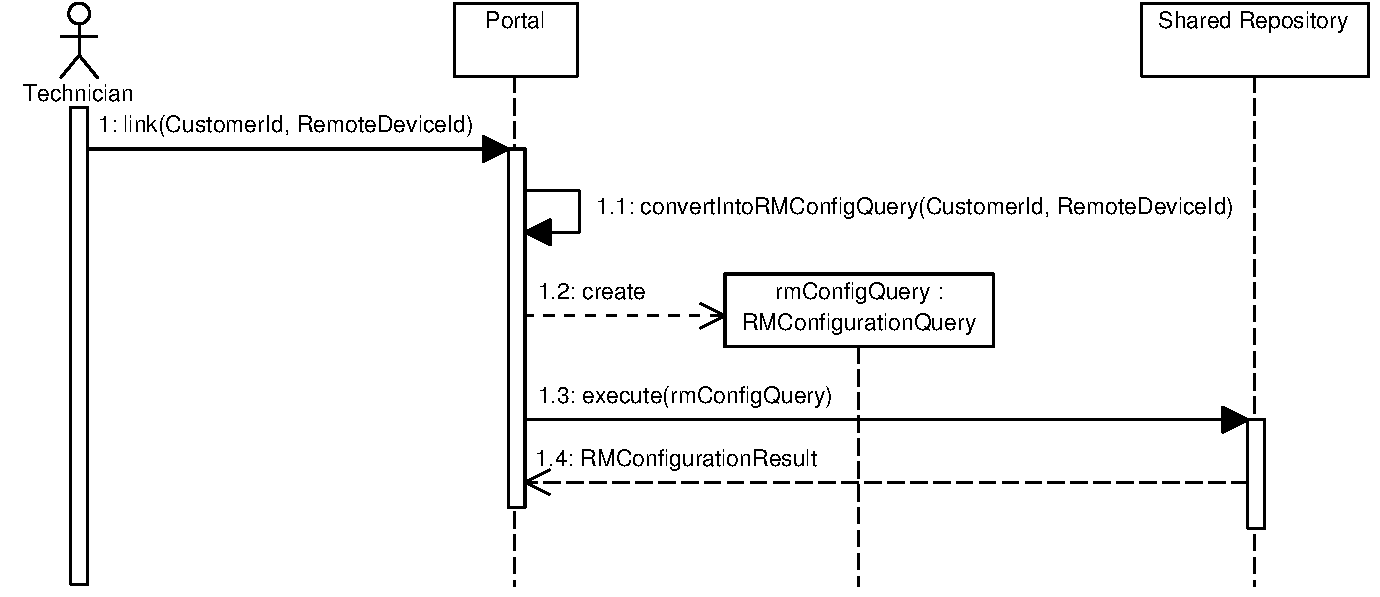
\includegraphics[width=\textwidth]{figs/scenario-5-2.pdf}
		\caption{Sequence diagram for the ``User profile association with a remote
		monitoring module'' scenario}
		\label{fig:scenario-5-2}
	\end{centering}
\end{figure}

\npar The query drafted in step 1.2 is a store query, which stores the contents
(i.e. the association) in the shared repository. The notification to the UIS of
the corresponding company is not executed since it was not mentioned in any of
the use cases.

\section{Remote monitoring: installation and initialization}
\label{scenario:rm-installation}

\npar Figure \ref{fig:scenario-5-3-1} shows the sequence diagram for the
scenario ``Remote monitoring: installation and initialization''. The physical
installation cannot be addressed in the diagram (it's not software). As a
replacement, the sequence diagram shows how a remote module is activated.

\begin{figure}[H]
	\begin{centering}
		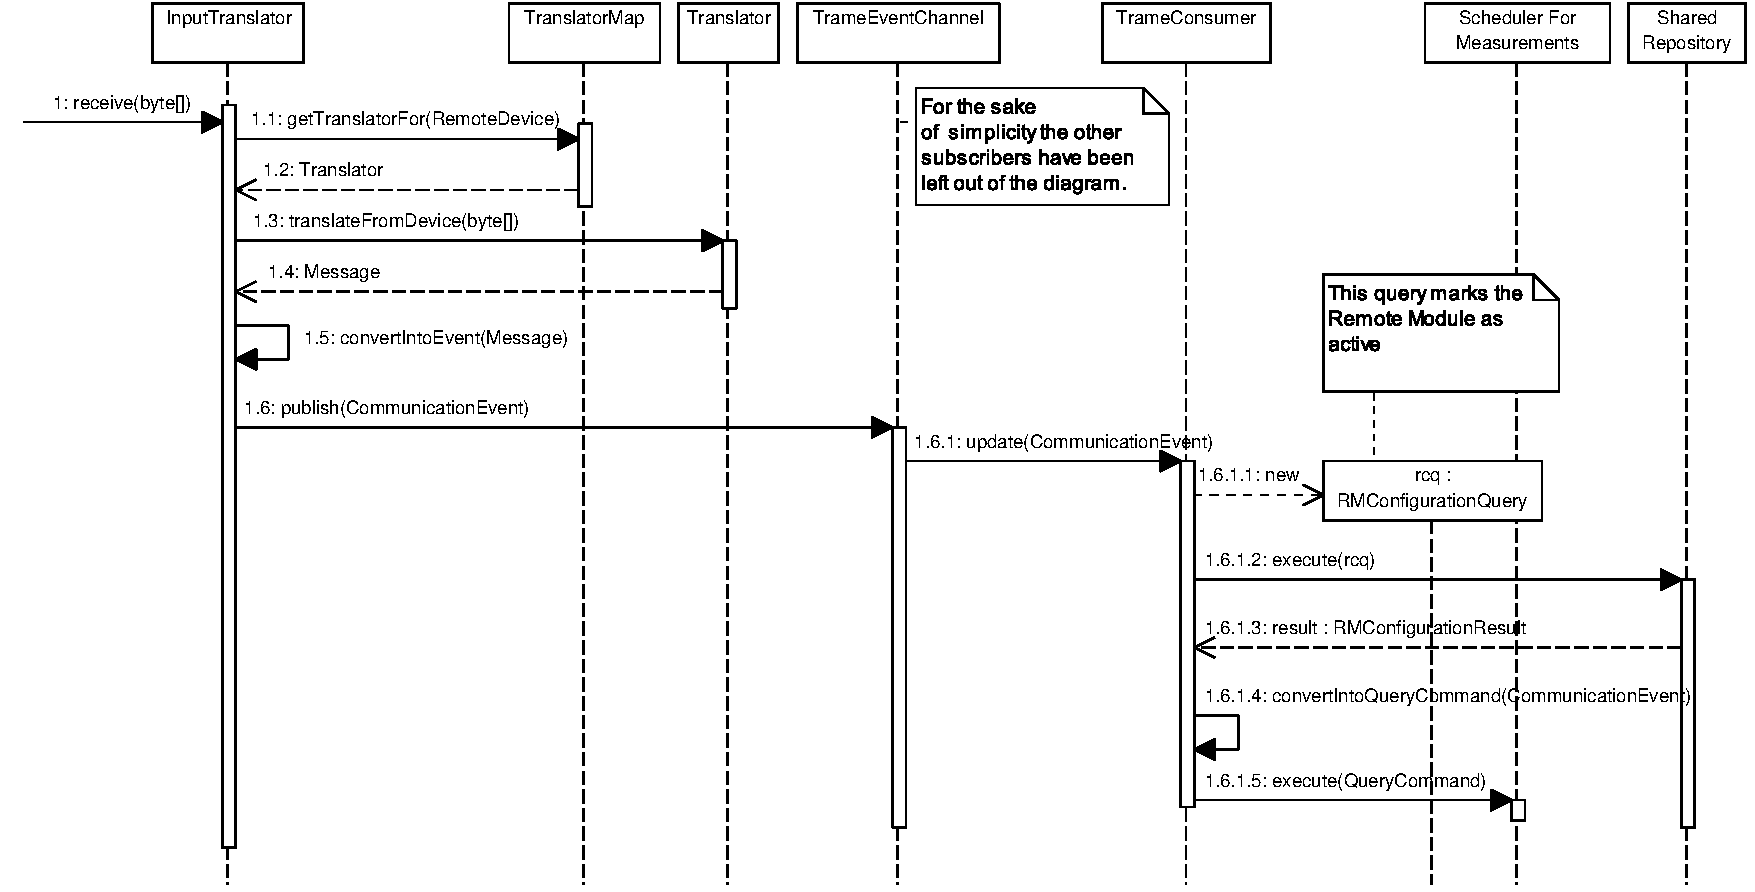
\includegraphics[width=\textwidth]{figs/scenario-5-3-1.pdf}
		\caption{Sequence diagram for the ``Remote monitoring: installation and
		initialization'' Scenario}
		\label{fig:scenario-5-3-1}
	\end{centering}
\end{figure}
\section{Transmission frequency reconfiguration}

\npar The sequence diagram of this scenario is splitted in two parts for the
sake of simplicity. The first part is an overview and the second diagram
contains a detailed diagram of the remote module communication unit.

\begin{figure}[H]
	\begin{centering}
		% TODO Figure
		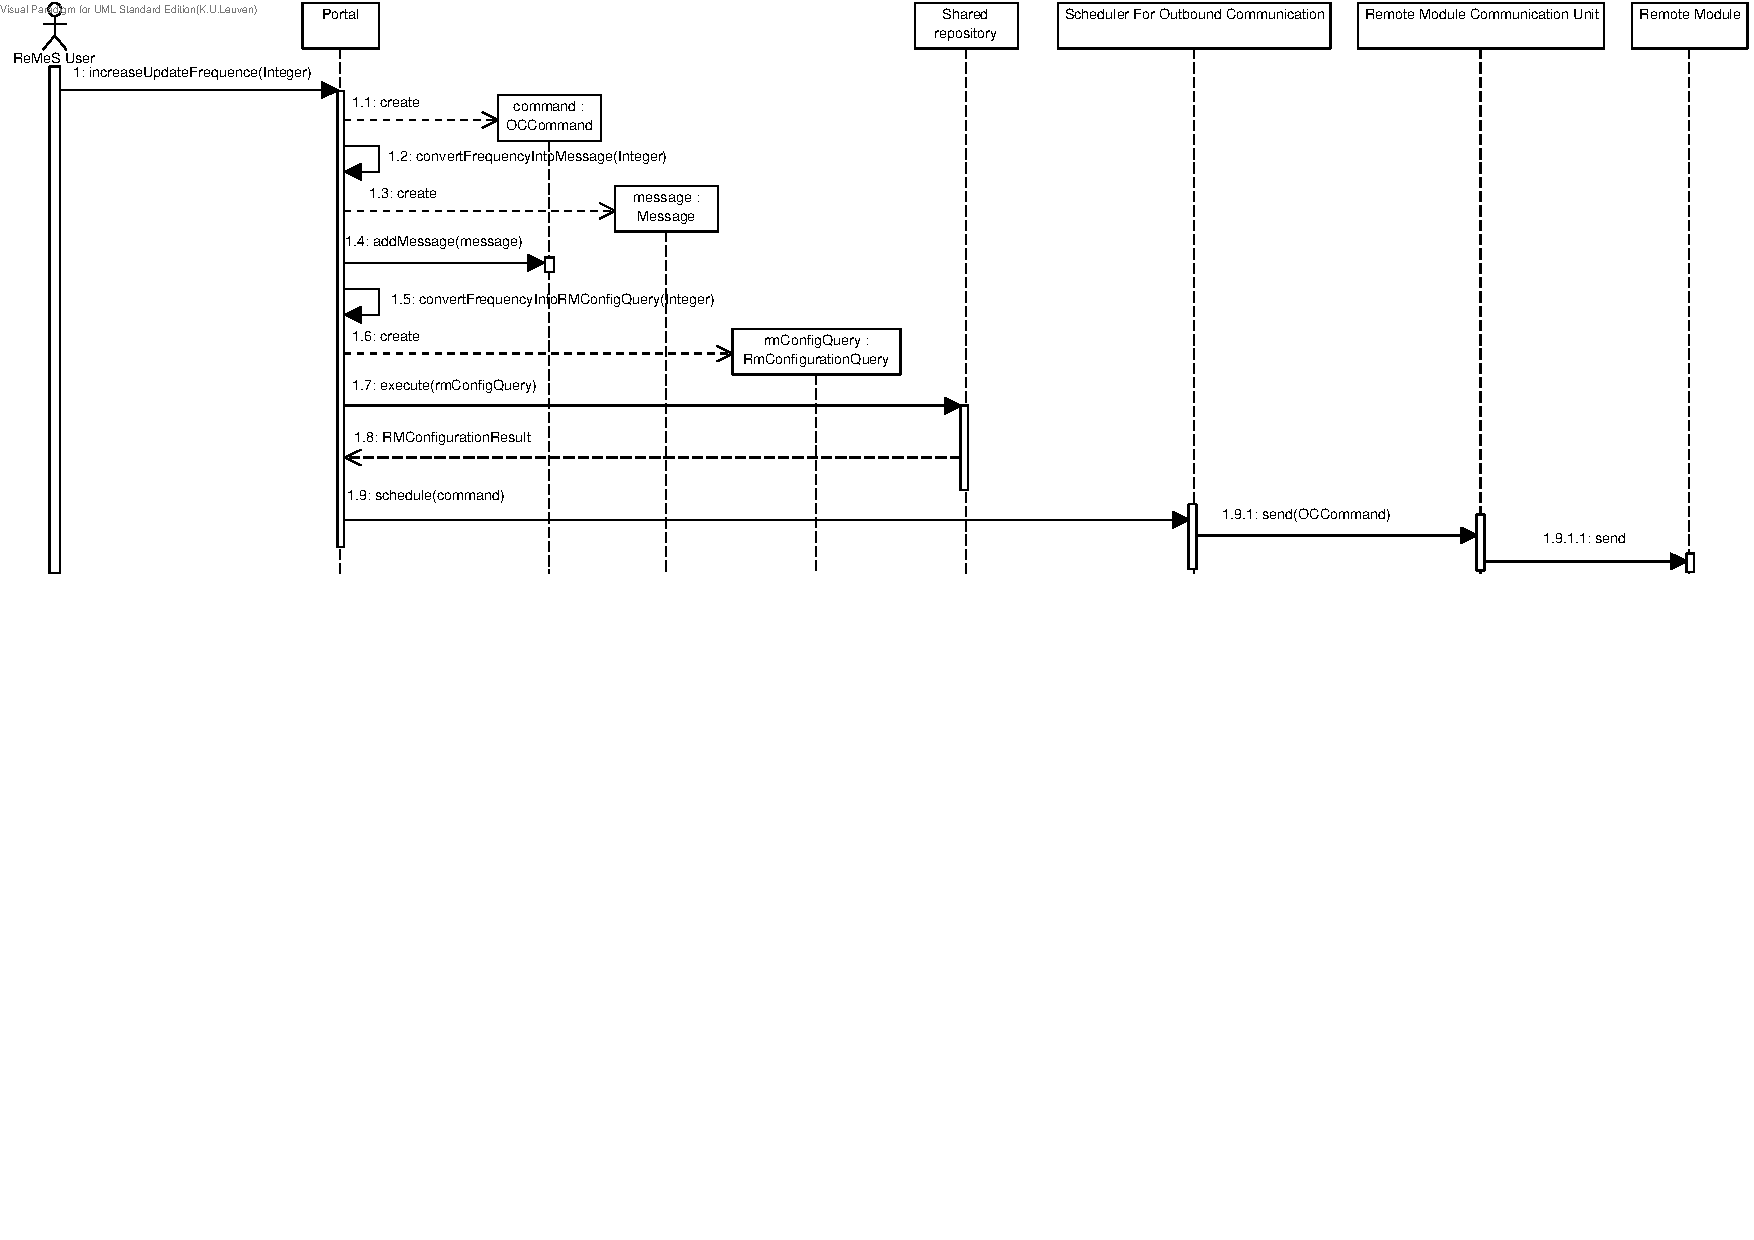
\includegraphics[width=\textwidth]{figs/scenario-5-3-2.pdf}
		\caption{The sequence diagram of scenario: Transmission frequency reconfiguration.}
		\label{fig:scenario-5-3-2}
	\end{centering}
\end{figure}

\npar In step 1.6, the drafted query is a store query for the new transmission
frequency. 

\begin{figure}[H]
	\begin{centering}
		% TODO Figure
		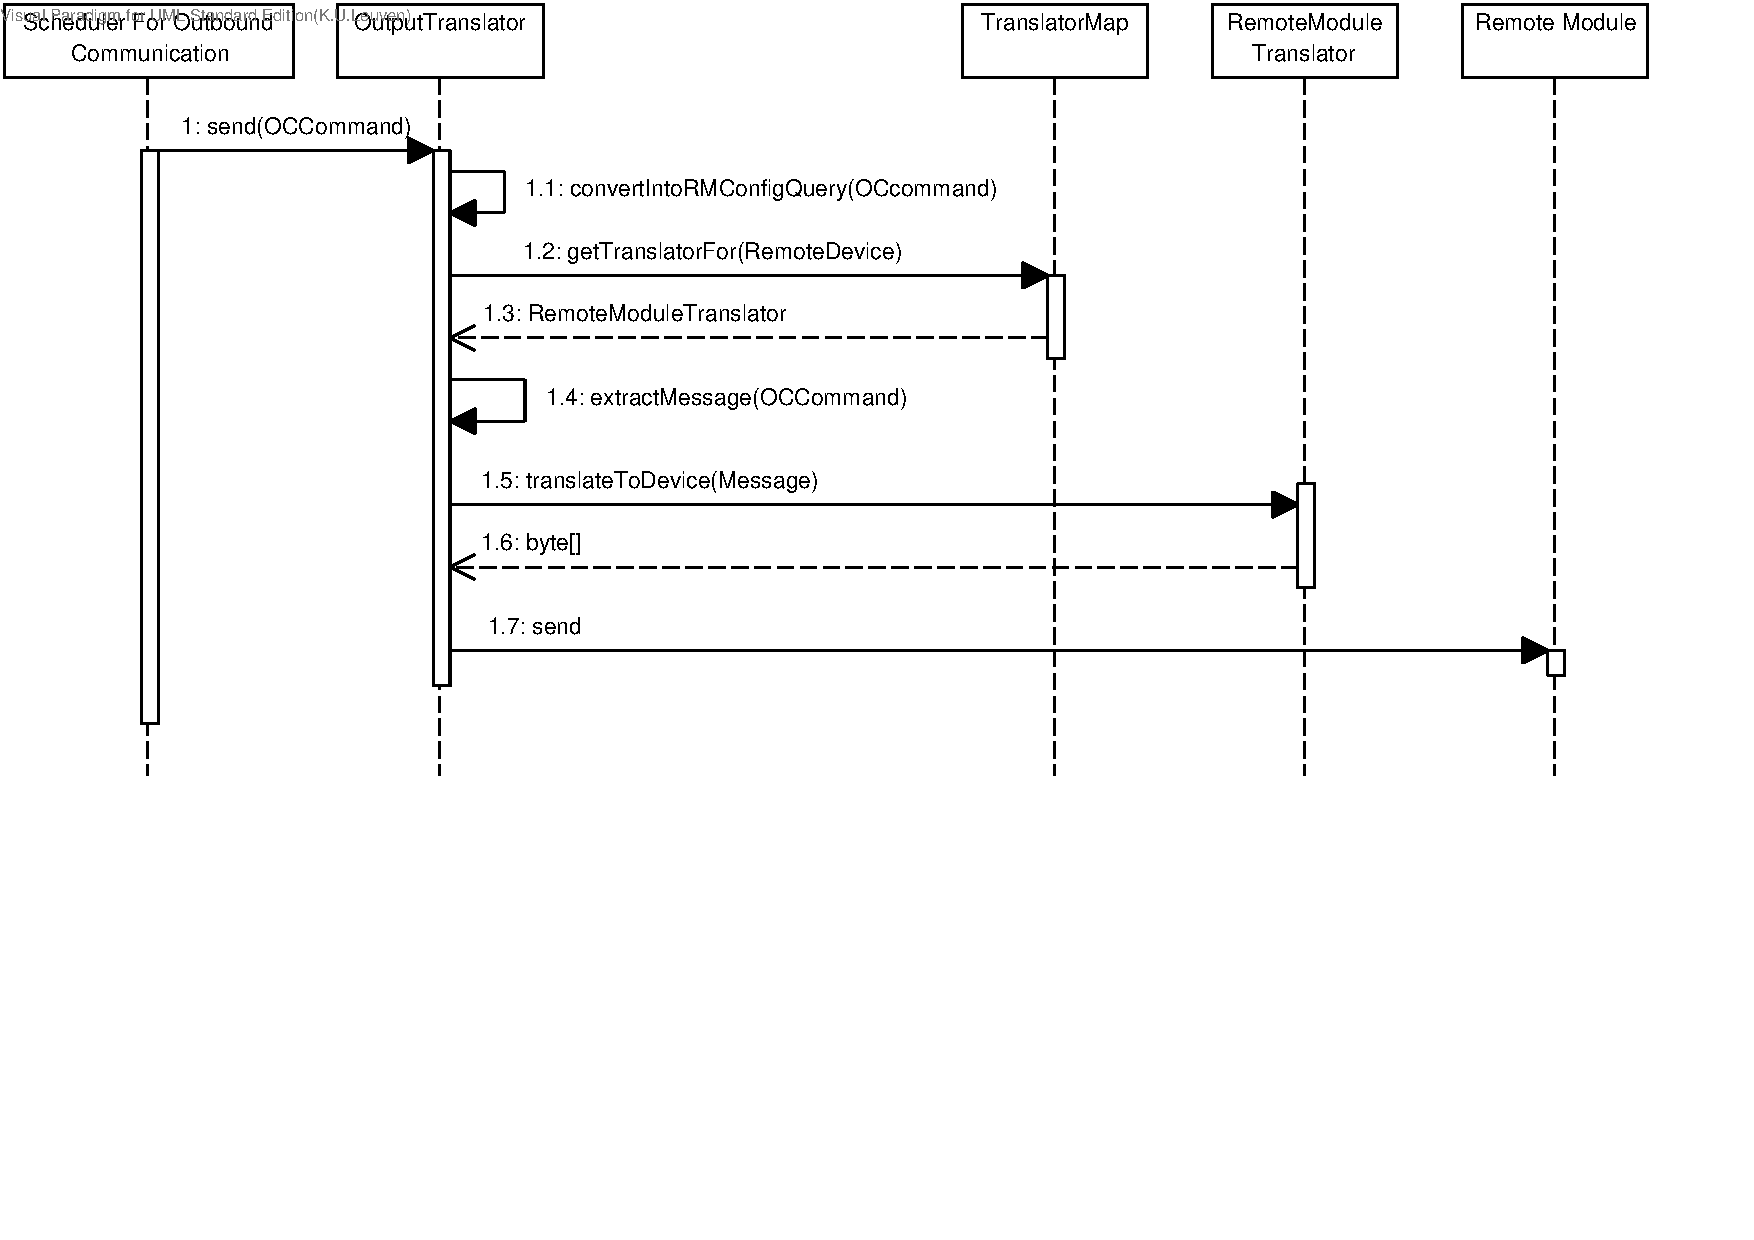
\includegraphics[width=\textwidth]{figs/scenario-5-3-2a.pdf}
		\caption{The sequence diagram of the remote module communication unit}
		\label{fig:scenario-5-3-2a}
	\end{centering}
\end{figure}

\npar The physical communication towards the remote module is modelled as a
``send'' message in the last step of diagram \ref{fig:scenario-5-3-2a}.

\section{Remote monitoring: troubleshooting}
\label{scenario:rm-troubleshooting}

\npar The ``Bill payment is received'' scenario mainly describes telephone
support after something went wrong with a remote module. Because this is not
software, we show what will happen when a measurement goes missing. Figure
\ref{fig:scenario-5-3-3} shows a sequence diagram for this scenario.

\begin{figure}[H]
	\begin{centering}
		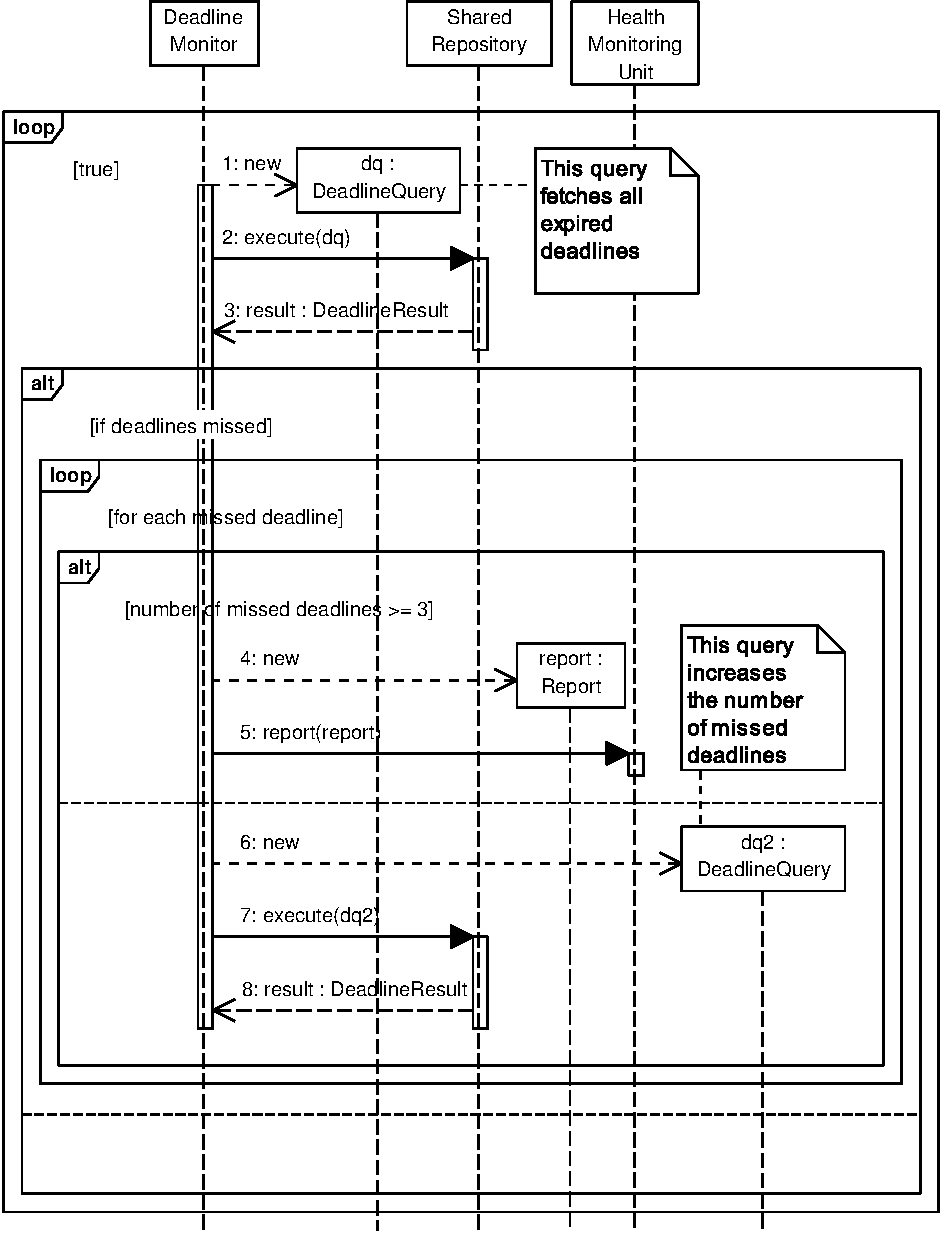
\includegraphics[width=\textwidth]{figs/scenario-5-3-3.pdf}
		\caption{Sequence diagram of the ``Remote monitoring: troubleshooting"
		Scenario}
		\label{fig:scenario-5-3-3}
	\end{centering}
\end{figure}

\npar At the arrival of a measurement trame, the deadline for the next trame is
calculated (update interarrival time + 10 minutes). Periodically, the
missed deadline are fetched from the database. For every device that missed the
deadline, a counter is increased. Whenever a counter for a device reaches 3, a
ReMeS operator is notified through the Health Monitoring Unit. 

\npar If, however, a trame arrives after the deadline, the counter is reset and
the next deadline is calculated and stored.

\section{Remote control}

\begin{figure}[H]
	\begin{centering}
		% TODO Figure
		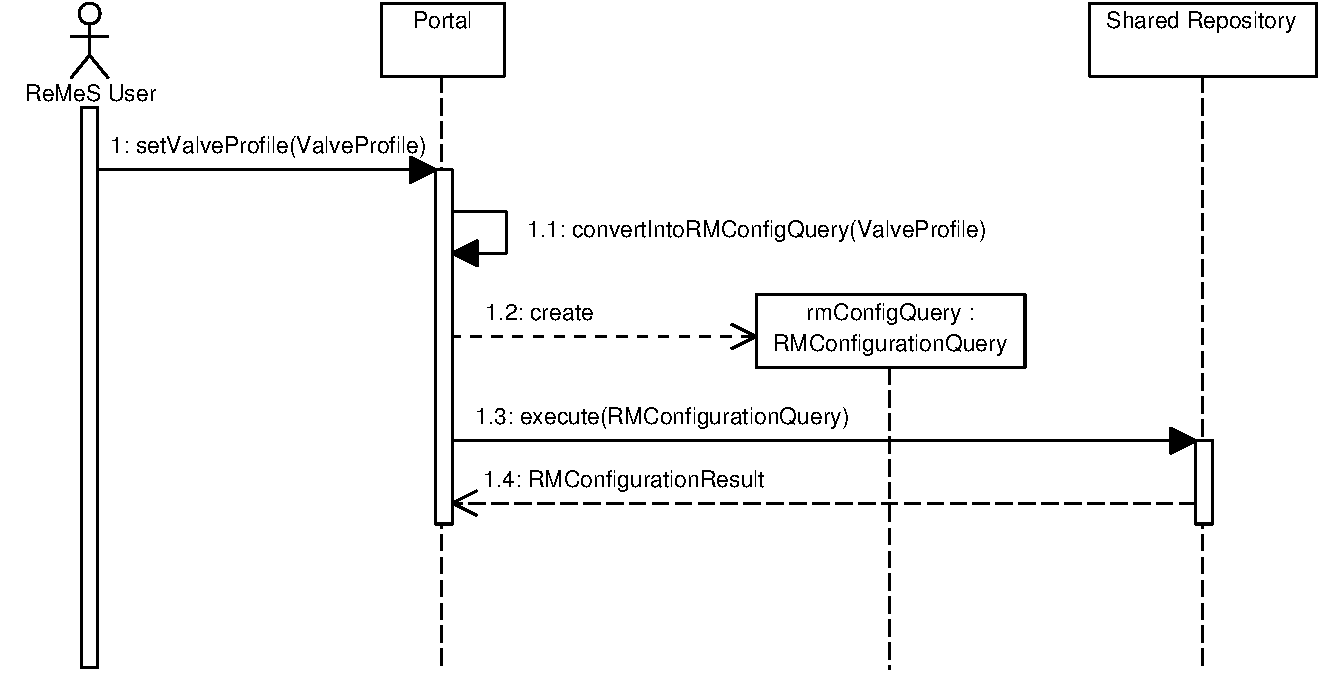
\includegraphics[width=\textwidth]{figs/scenario-5-4.pdf}
		\caption{The sequence diagram of scenario: Remote control.}
		\label{fig:scenario-5-4}
	\end{centering}
\end{figure}

\npar The RMConfigurationQuery is a store query to store the new profile. Hence,
the RMConfigurationResult is empty.

\section{Normal measurements data transmission}
\label{scenario:measurements-transmission}

\npar The interactions from this scenario are included in scenario
\ref{scenario:data-analysis}. 

\section{Individual data analysis}
\label{scenario:data-analysis}

\npar The sequence diagram of this scenario is divided into several subsequence
diagrams. This is done to prevent overloading when trying to place everything
into one diagram. First of all an overview diagram is given using only high
level components (i.e. components which are further decomposed in a separate
iteration). In the other diagrams we zoom in on a number of components from the
first diagram. The scheduler components are not detailed any further since they
do not modify the format of the incoming parameters, they just do the
scheduling.

\npar In the text of the scenario a ``consumption profile'' is mentioned. We
assumed that this is a profile belonging to a customer which contains all
anomalies of that customer. This looks strange at first sight, but it is the
only option we saw as it could not be the measurements of that customer (cfr.
the text).

\begin{figure}[H]
	\begin{centering}
		% TODO Figure
		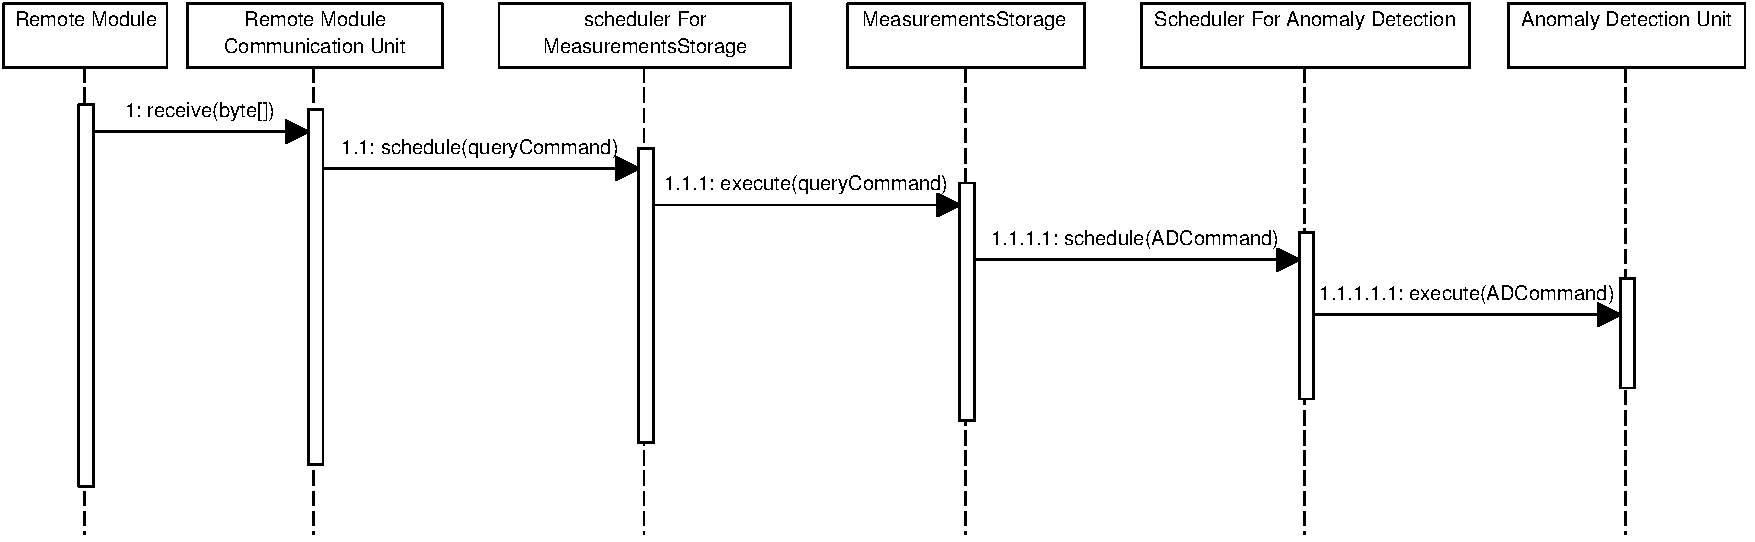
\includegraphics[width=\textwidth]{figs/scenario-5-6.pdf}
		\caption{Overview sequence diagram for the ``Individual data analysis''
		scenario}
		\label{fig:scenario-5-6}
	\end{centering}
\end{figure}

\begin{figure}[H]
	\begin{centering}
		% TODO Figure
		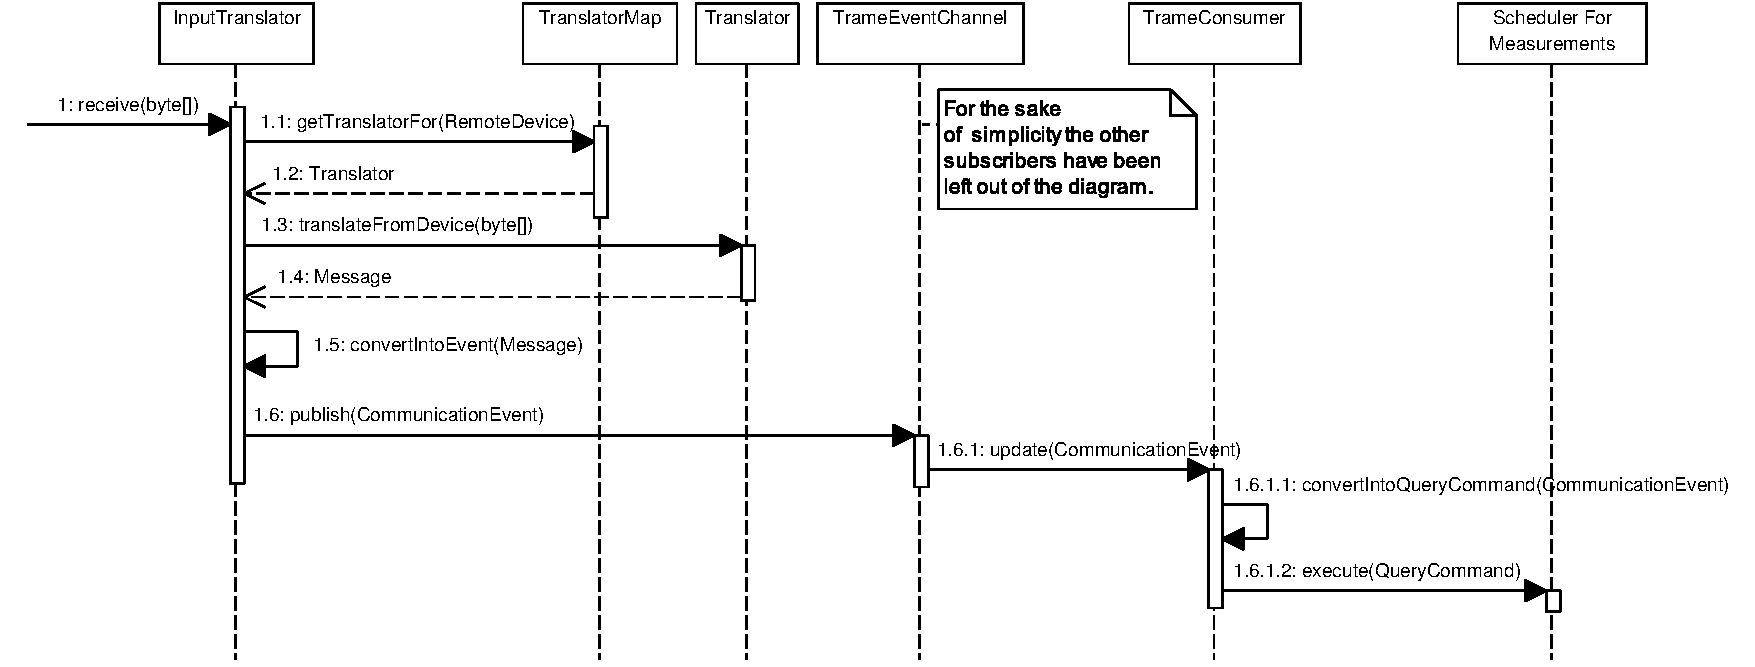
\includegraphics[width=\textwidth]{figs/scenario-5-6a.pdf}
		\caption{Detailed sequence diagram for the Remote Module Communication Unit}
		\label{fig:scenario-5-6a}
	\end{centering}
\end{figure}

\begin{figure}[H]
	\begin{centering}
		% TODO Figure
		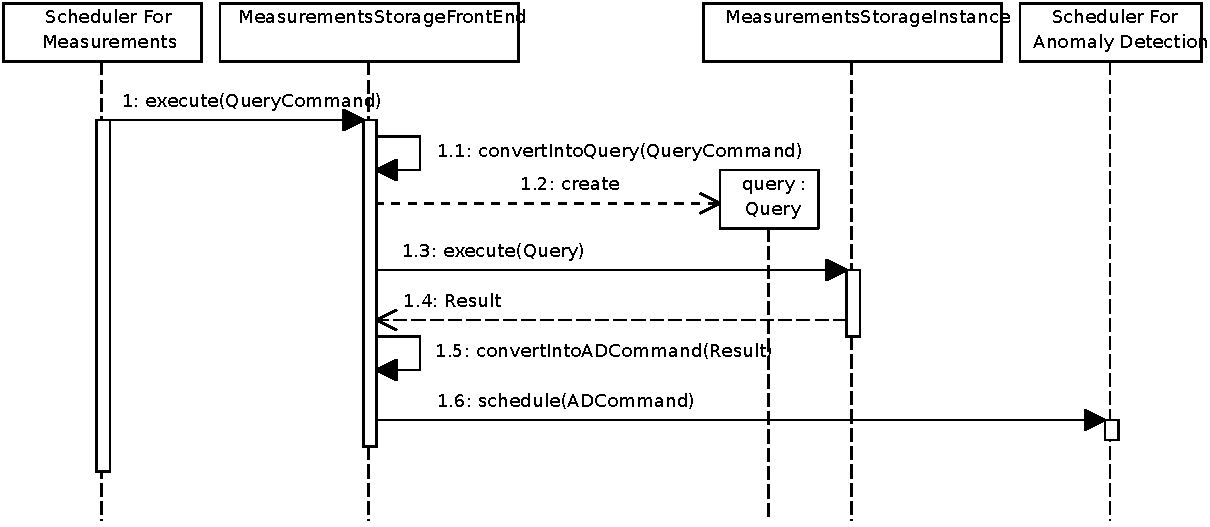
\includegraphics[width=\textwidth]{figs/scenario-5-6b.pdf}
		\caption{Detailed sequence diagram for Measurements Storage}
		\label{fig:scenario-5-6b}
	\end{centering}
\end{figure}

\npar The query in step 1.2 of figure \ref{fig:scenario-5-6b} is a store query
to store the incoming measurement.

\begin{figure}[H]
	\begin{centering}
		% TODO Figure
		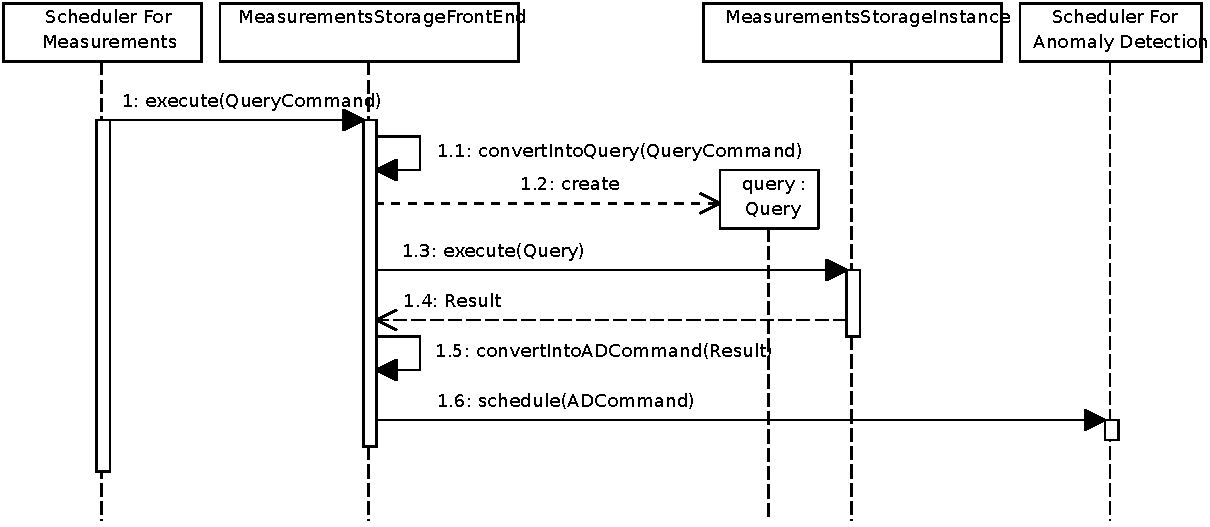
\includegraphics[width=\textwidth]{figs/scenario-5-6b.pdf}
		\caption{Detailed sequence diagram for the Anomaly Detection Unit}
		\label{fig:scenario-5-6c}
	\end{centering}
\end{figure}

\npar In step 1.4 a read query is constructed to gain additional measurement
data belonging to the same remote module. The \method{addMeasurements()} method
will add the retrieved measurements to the ADCommand. In step 1.7 there is
another query constructed to store the results of the analysis. Once again this
means that the AlarmResult is empty.




\section{Utility production planning analysis}
\label{scenario:production-planning}

\npar Figure \ref{fig:scenario-5-7} shows a sequence diagram for the ``Utility
production planning analysis'' scenario. All measurement data for some period is
fetched and processed. The prediction is saved in the ReMeS database.

\begin{figure}[H]
	\begin{centering}
		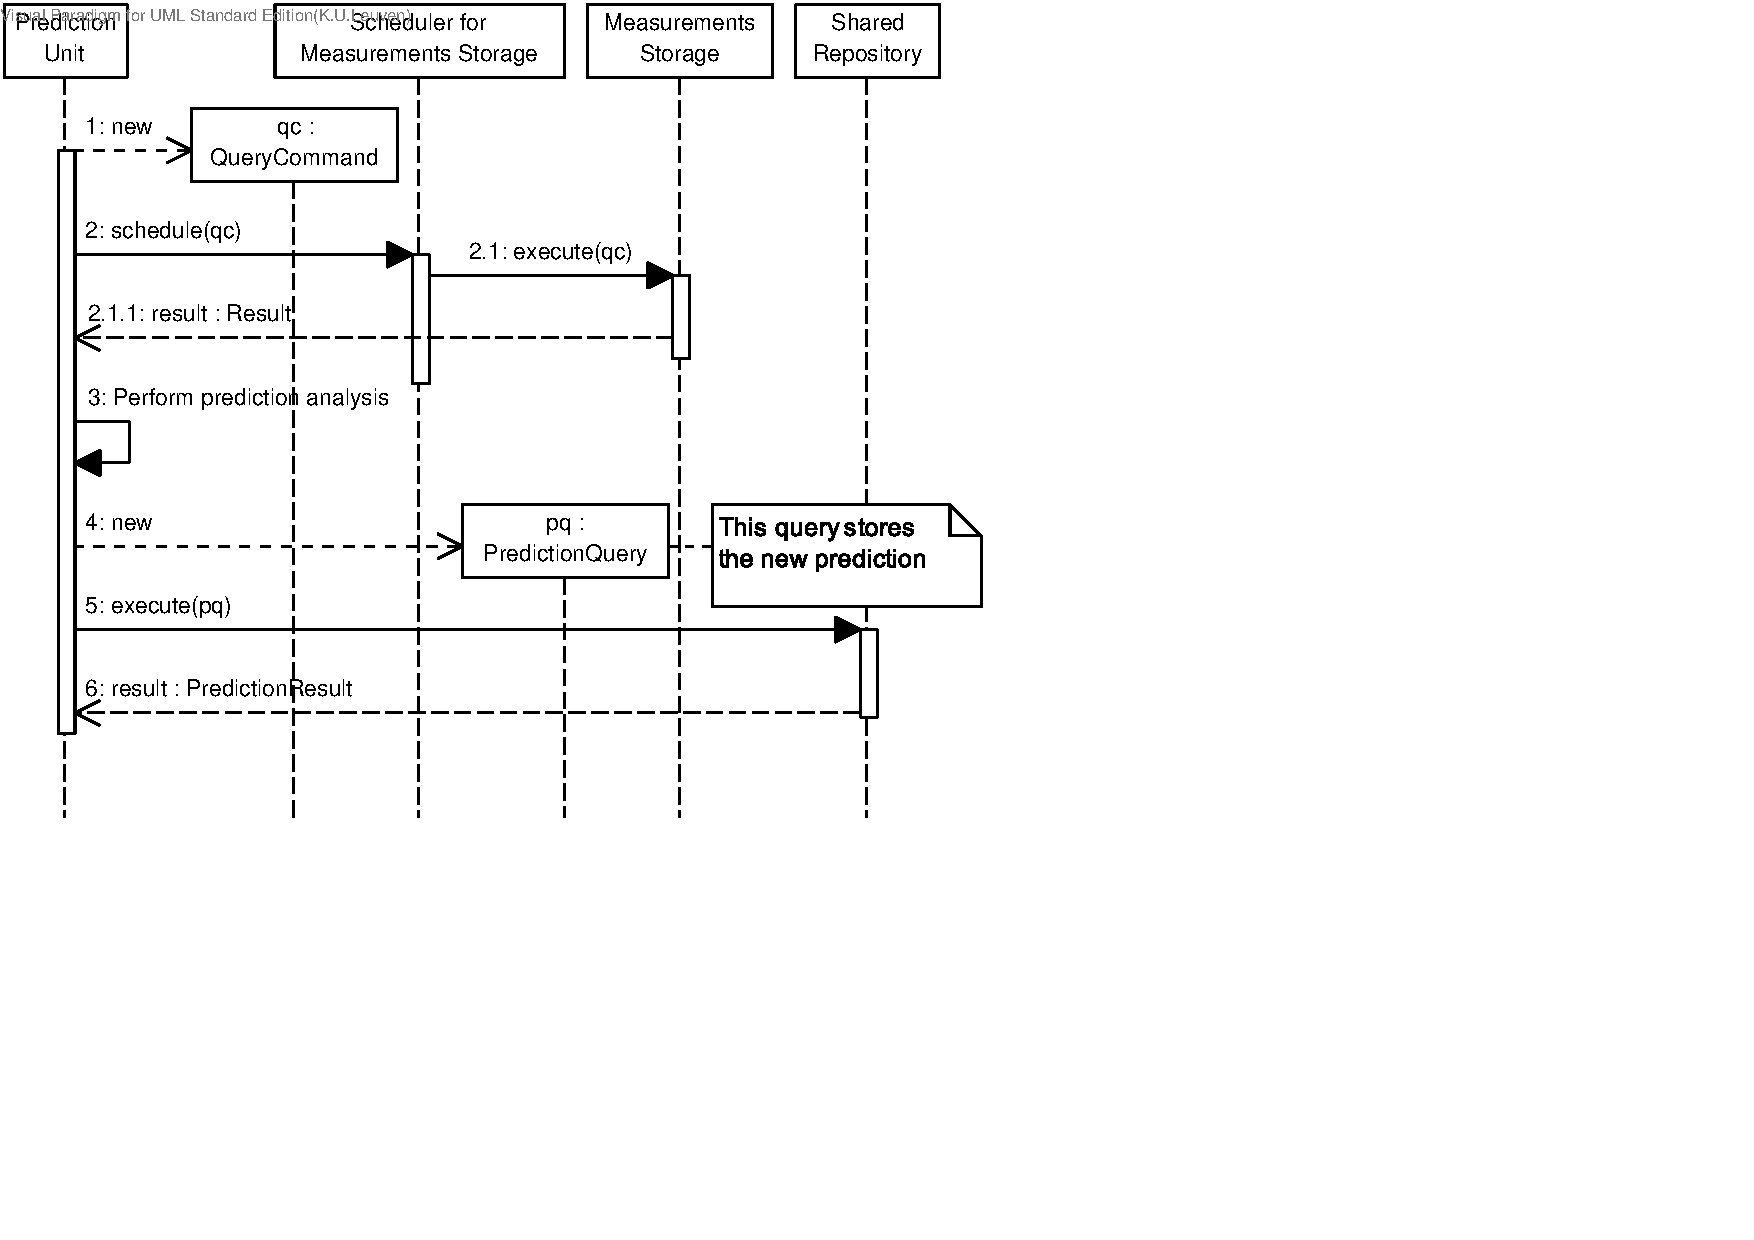
\includegraphics[width=0.7\textwidth]{figs/scenario-5-7.pdf}
		\caption{Sequence diagram for the ``Utility production planning analysis'' scenario}
		\label{fig:scenario-5-7}
	\end{centering}
\end{figure}

\section{Information exchange towards the UIS}

\npar Figure \ref{fig:scenario-5-8} shows the sequence diagram for the scenario
``Information exchange towards the UIS''.

\begin{figure}
	\begin{centering}
		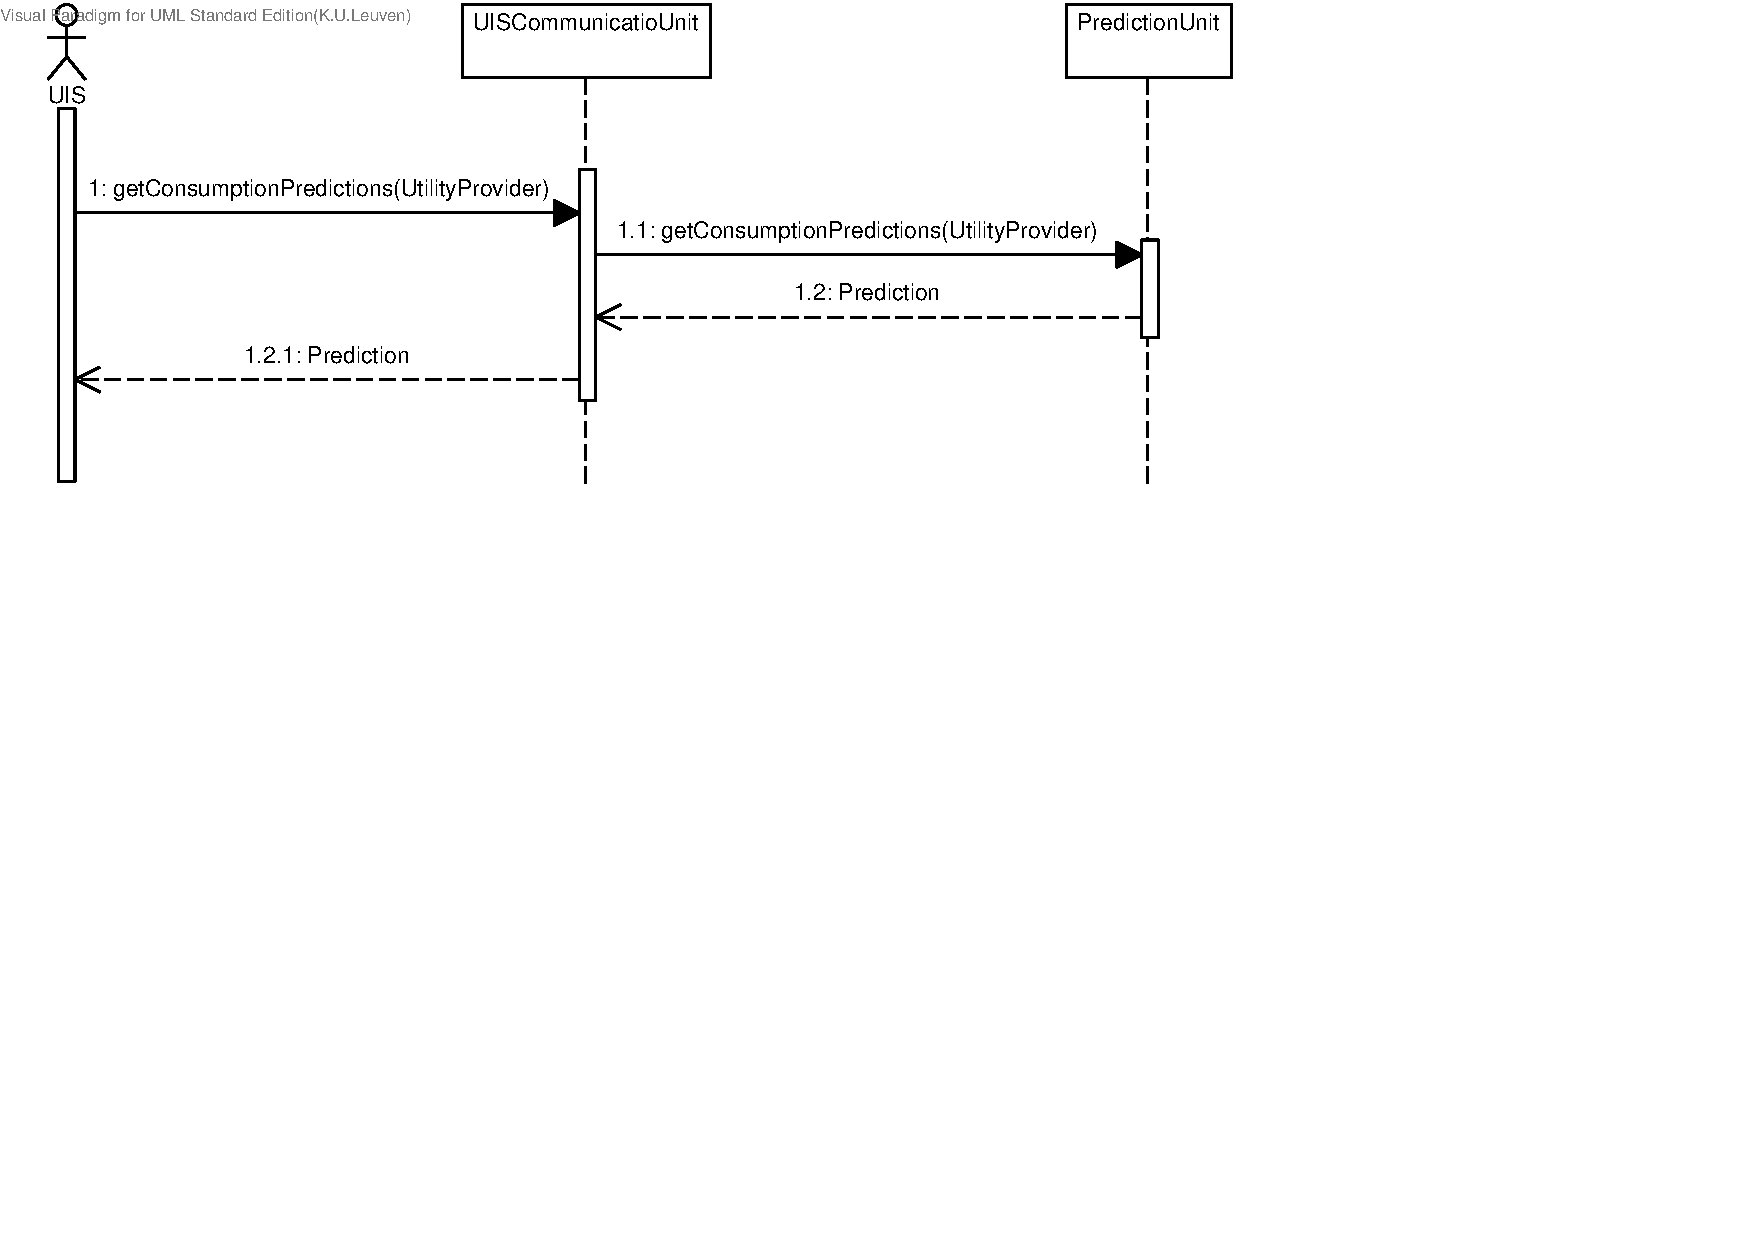
\includegraphics[width=\textwidth]{figs/scenario-5-8.pdf}
		\caption{Sequence diagram for the ``Information exchange towards the UIS''
		scenario}
		\label{fig:scenario-5-8}
	\end{centering}
\end{figure}

\npar Notice that the sequence is started by the UIS in contradiction to the
text in the scenario. The action is inverted because it was stated so in use
case 14 (Request consumption predictions). It is further important to remark
that the inverted situation could easily be modelled in our architecture (but
again this is not done to remain consistent with the use cases).

\npar The consumption demands also can't be retrieved since it was again not
mentioned in any of the use cases. Providing this functionality, however, would
not form a problem at all.

\section{Alarm data transmission: remote monitoring module}
\label{scenario:rm-alarm}

\npar Figure \ref{fig:scenario-5-9} shows a sequence diagram for the ``Alarm
data transmission: remote monitoring module'' scenario. For every incoming
alarm trame, the trame is checked for a false positive by the anomaly detection
unit (only the case of a real alarm is shown), the valve is shut and the alarm
recipients are notified.

\begin{figure}[H]
	\begin{centering}
		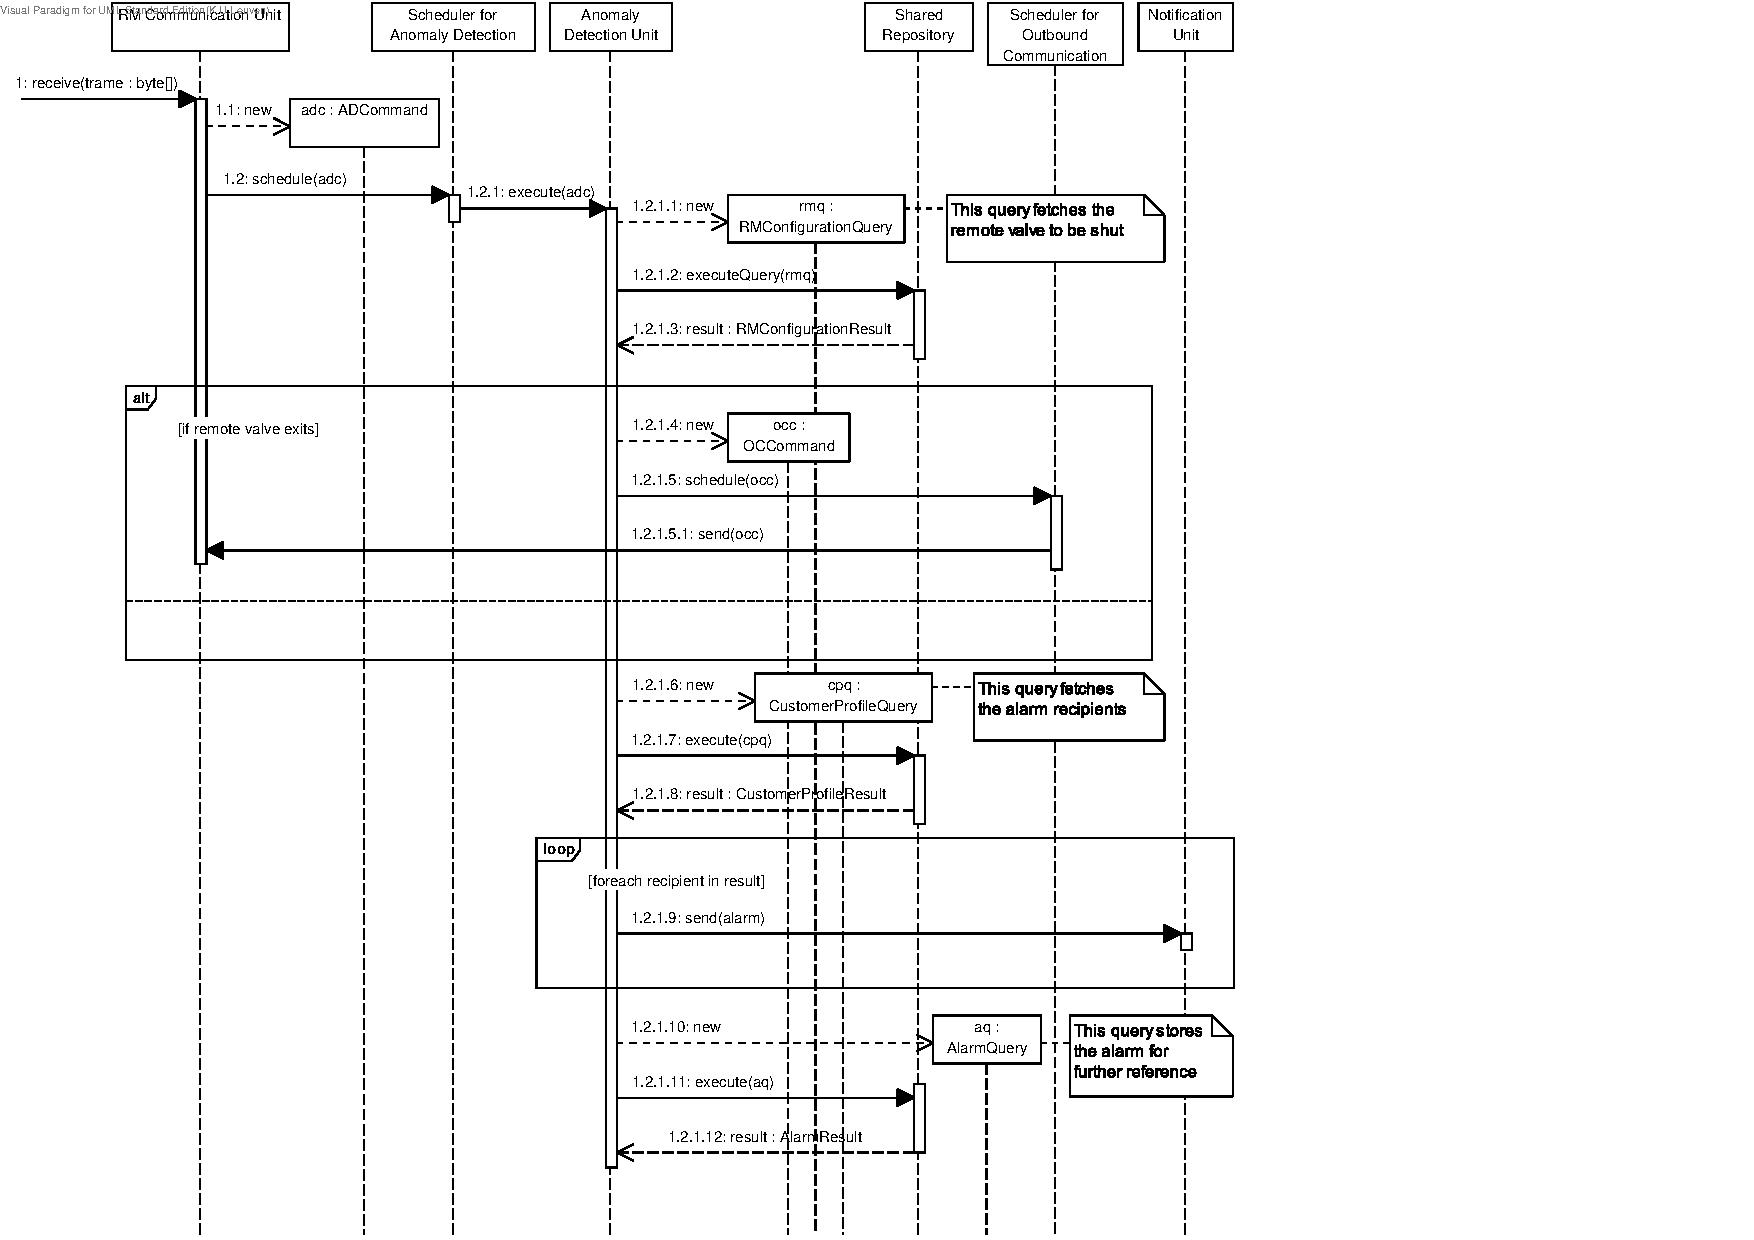
\includegraphics[width=\textwidth]{figs/scenario-5-9.pdf}
		\caption{Sequence diagram for the ``Alarm data transmission: remote monitoring
		module'' scenario}
		\label{fig:scenario-5-9}
	\end{centering}
\end{figure}
\section{Alarm data transmission: ReMeS}
\label{scenario:remes-alarm}

\npar Figure \ref{fig:scenario-5-10} shows the sequence diagram for the scenario
``Alarm data transmission: ReMeS''.

\begin{figure}[H]
	\begin{centering}
		% TODO Figure
		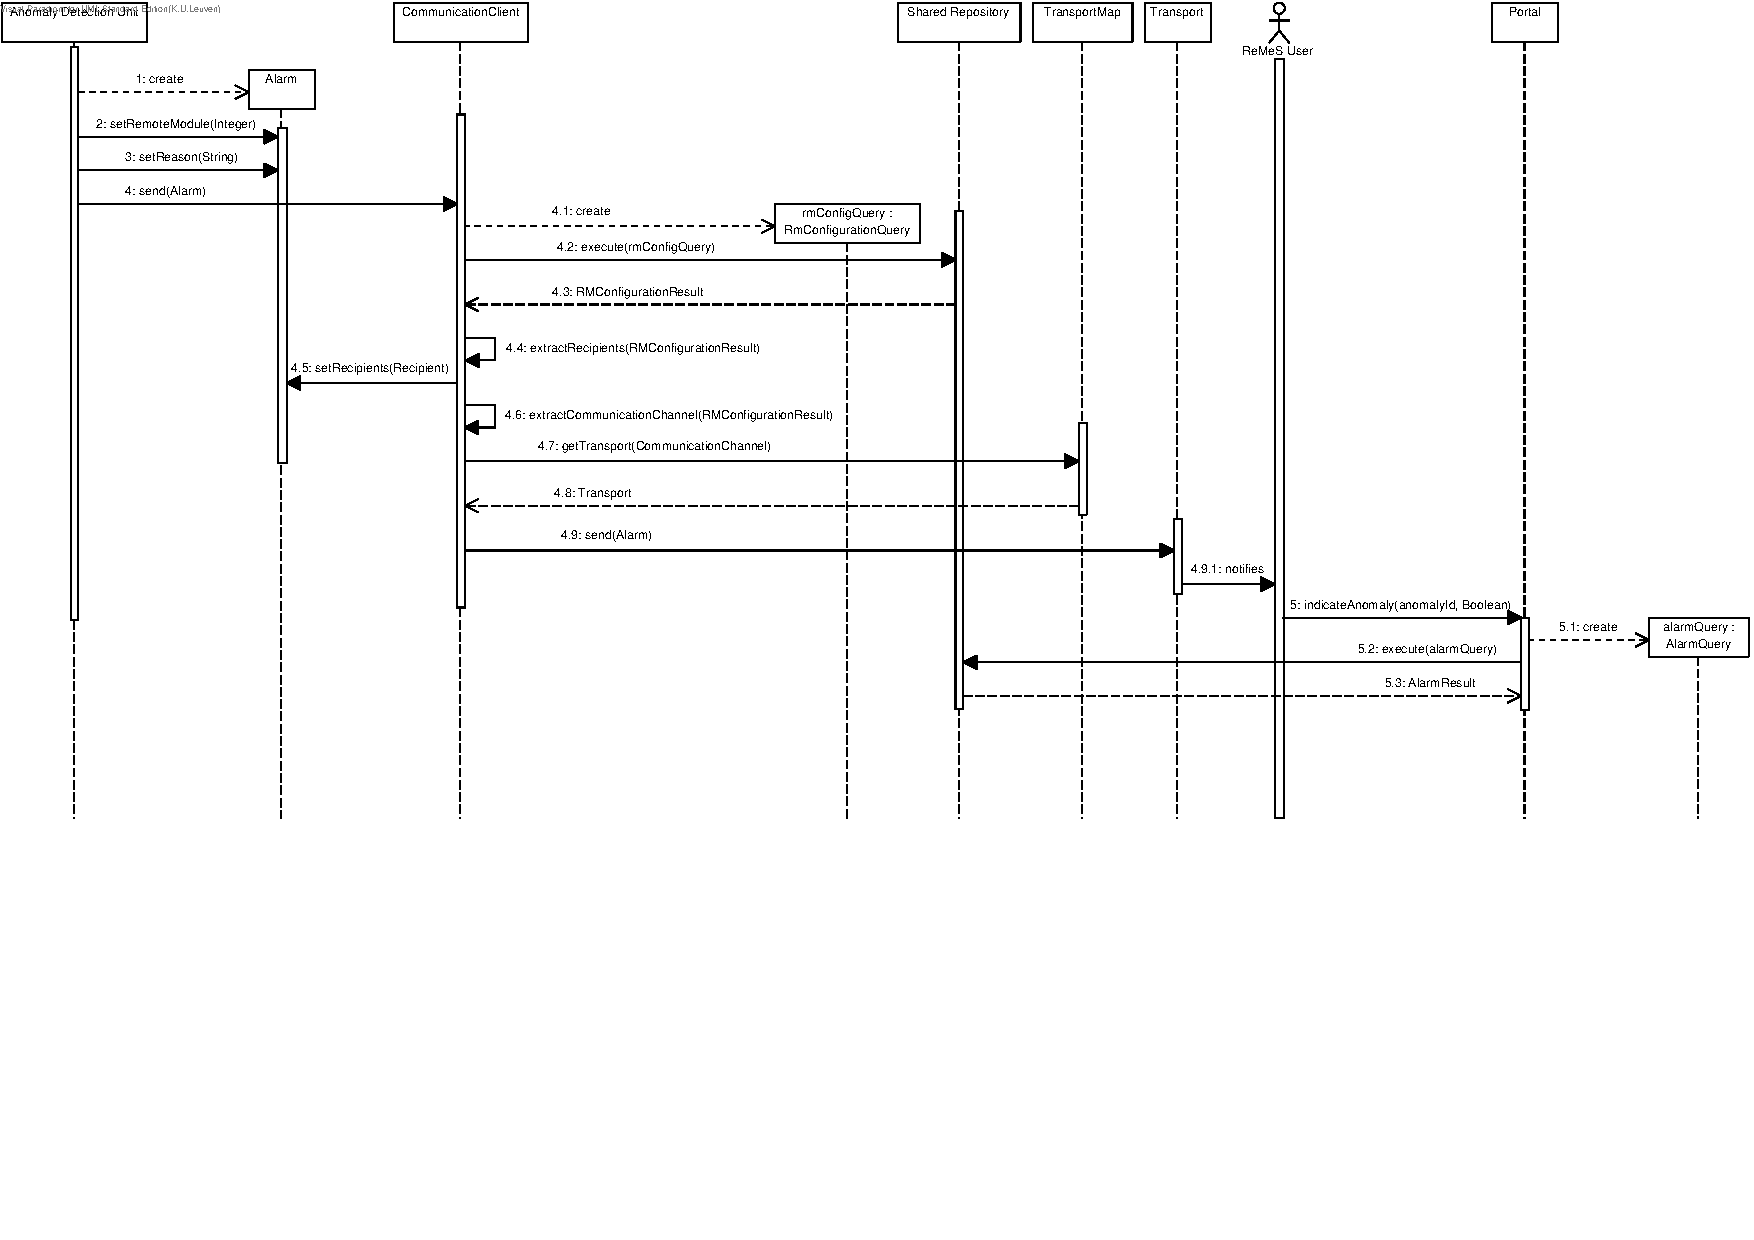
\includegraphics[width=\textwidth]{figs/scenario-5-10.pdf}
		\caption{Sequence diagram for the ``Alarm data transmission: ReMeS'' scenario}
		\label{fig:scenario-5-10}
	\end{centering}
\end{figure}

\npar In step 4.1 a RemoteModuleConfigurationQuery is drafted. This is a read
query to retrieve the configuration of the remote module (which is contained in
the Alarm). This configuration contains the alarm recipients and the
communication channel.

\npar In step 5 a ``notifies'' message is drawn to indicate that the ReMeS user
is physically contacted.

\npar In step 5.1 a store query is constructed. This query contains whether or
not the detected anomaly was correct. The returned result (AlarmResult) is empty
since it is a store query.


\section{Remote control module de-activation}

\npar Figure \ref{fig:scenario-5-12} shows the sequence diagram for the scenario
``Remote control module de-activation''.

\begin{figure}[H]
	\begin{centering}
		% TODO Figure
		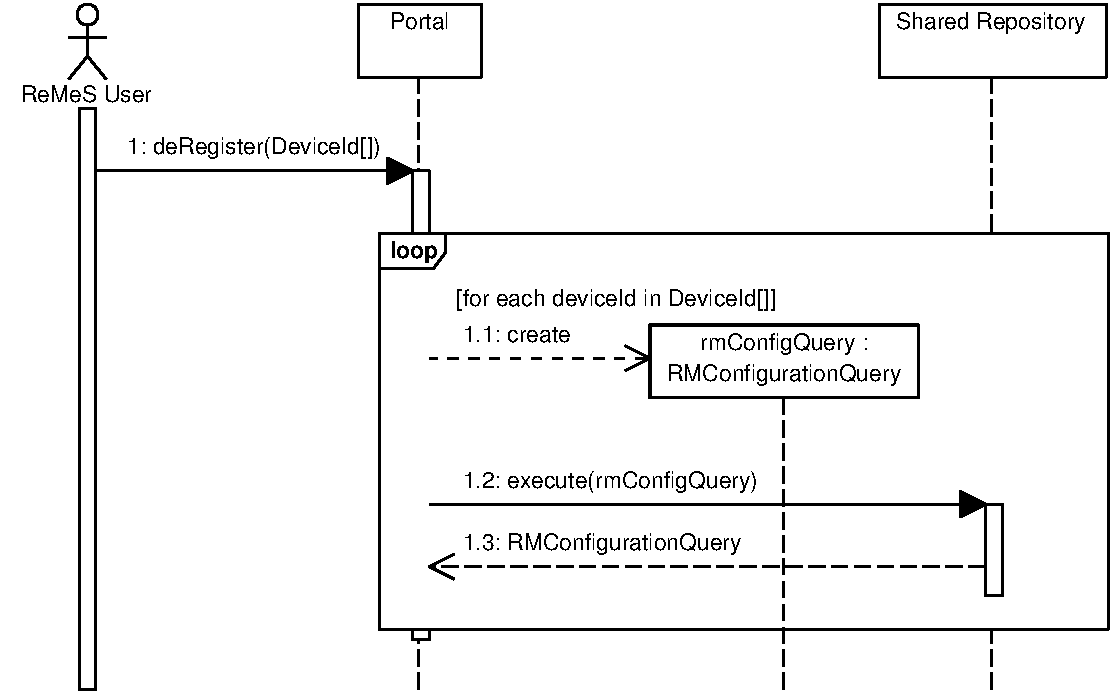
\includegraphics[width=\textwidth]{figs/scenario-5-12.pdf}
		\caption{Sequence diagram for the ``Remote control module de-activation''
		scenario}
		\label{fig:scenario-5-12}
	\end{centering}
\end{figure}

\npar In step 1.1 of figure \ref{fig:scenario-5-12} an RMConfiguarionQuery is
made. This query contains the deviceId to be unregistered, so it is an
update query. This means that the result, RMConfigurationQuery, will in fact be
empty.

\section{New Bill Creation}
\label{scenario:bill-creation}

\begin{figure}[H]
	\begin{centering}
		% TODO Figure
		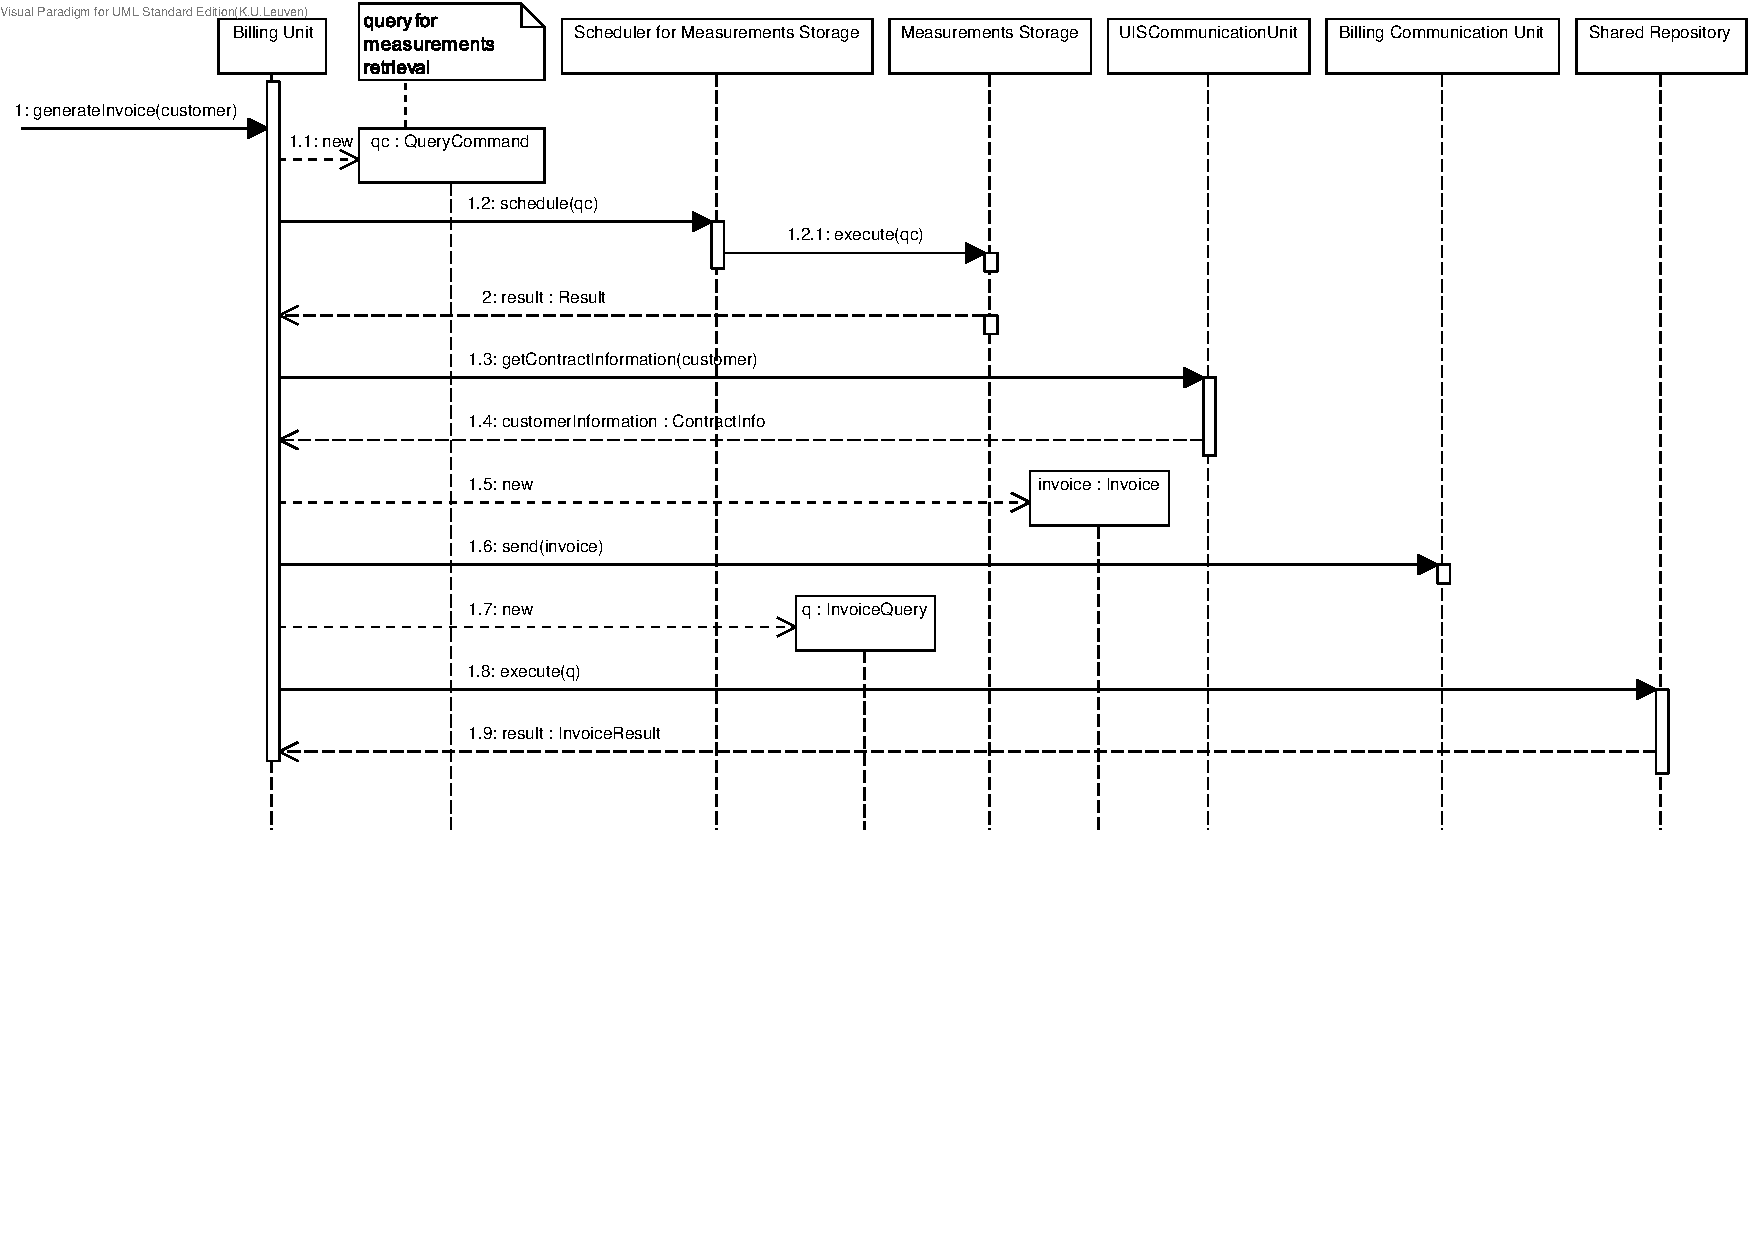
\includegraphics[width=\textwidth]{figs/scenario-5-13.pdf}
		\caption{The sequence diagram of scenario ``New bill creation''}
		\label{fig:scenario-5-14}
	\end{centering}
\end{figure}

\section{Bill payment is received}
\label{scenario:bill-paid}

\npar Figure \ref{fig:scenario-5-14} shows the sequence diagram for the scenario
``Bill payment is received''.

\begin{figure}[H]
	\begin{centering}
		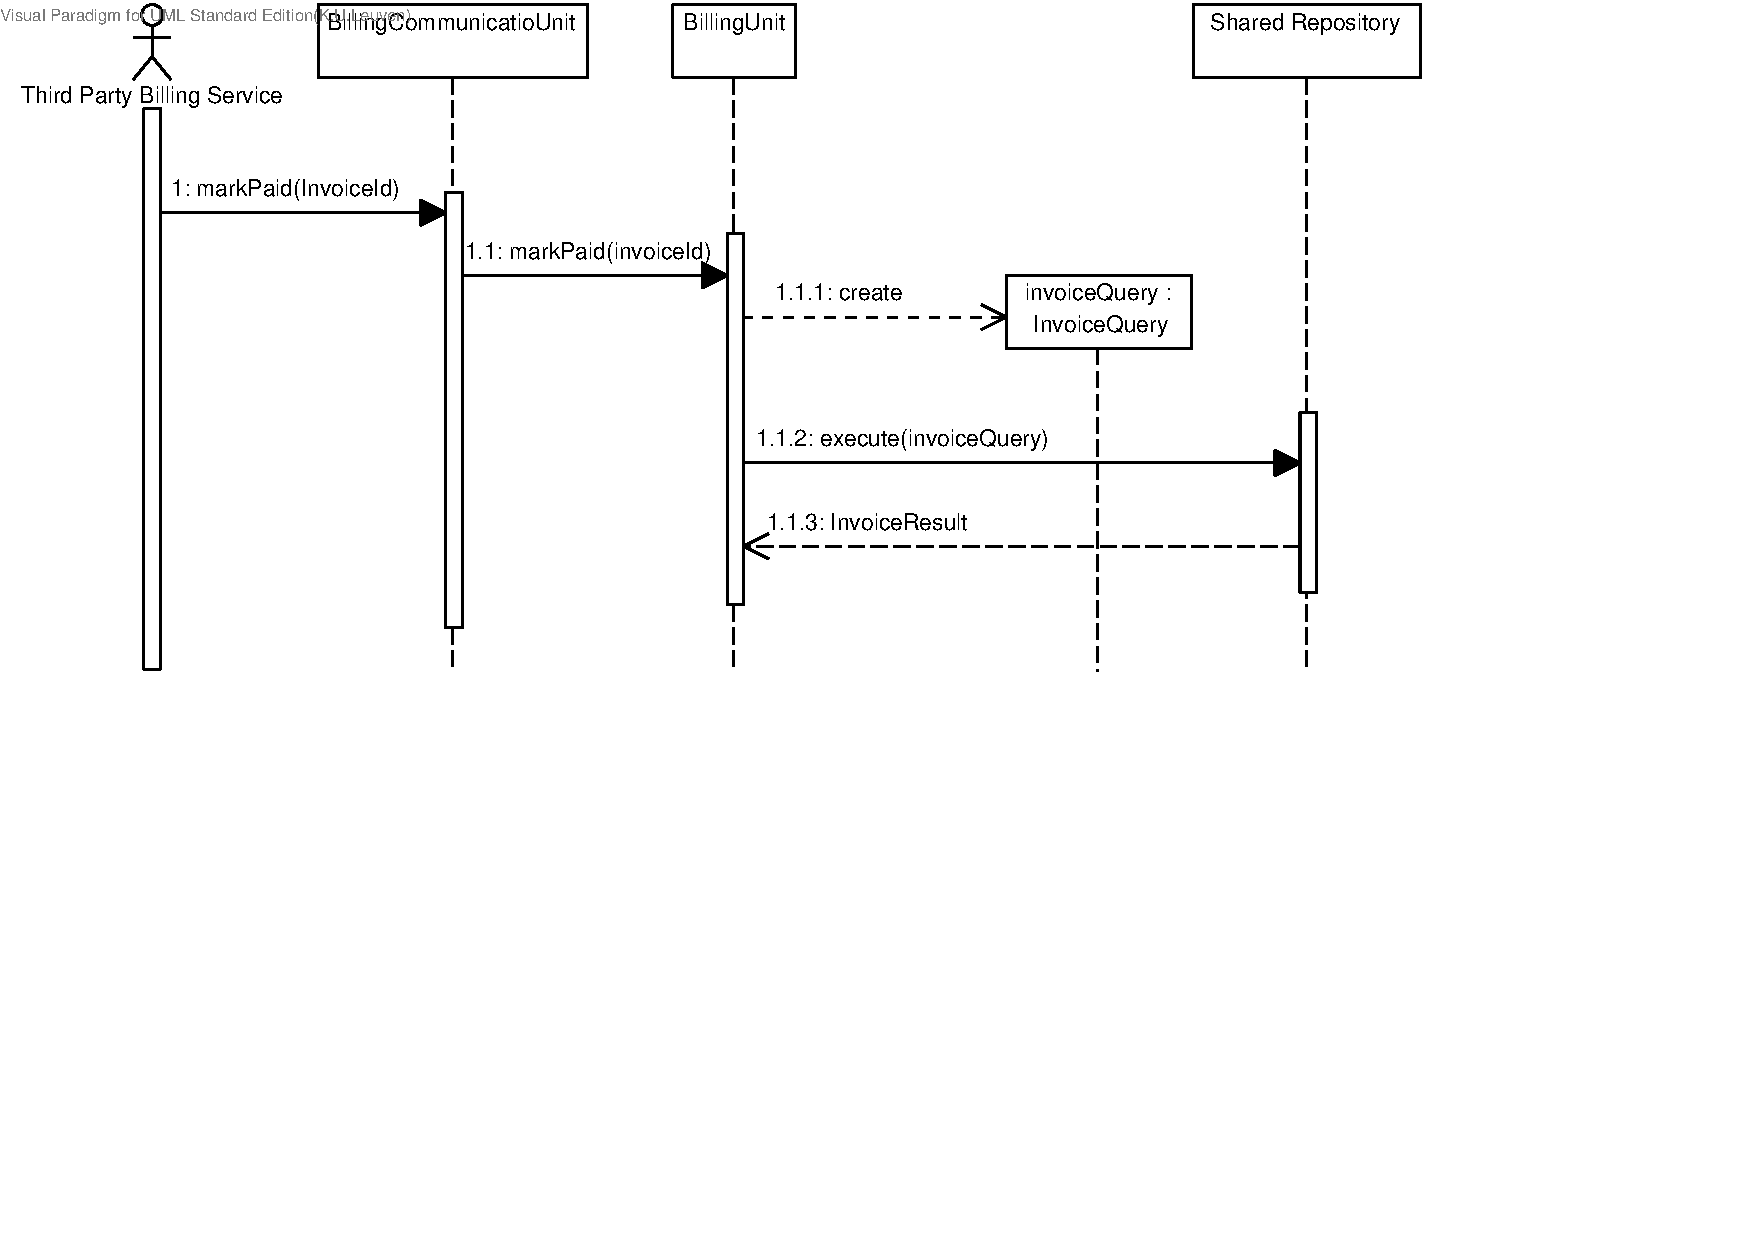
\includegraphics[width=\textwidth]{figs/scenario-5-14.pdf}
		\caption{Sequence diagram for the ``Bill payment is received'' scenario}
		\label{fig:scenario-5-14}
	\end{centering}
\end{figure}

\npar In step 1.1.1 of figure \ref{fig:scenario-5-14} an InvoiceQuery is
created. This query contains the invoiceId and the message that that invoice is
paid. The query is an update query, so the result that is returned
(InvoiceResult) will in fact be empty.


\appendix

\chapter{Element Catalog}
\label{chap:element-catalog}

\section{Scheduler For Measurements}
\label{element:measurements-scheduler}

\subsection{Roles and responsibilities}

\npar This scheduler has to regulate all the traffic of QueryCommand towards the
MeasurementsStorage. It accepts incoming QueryCommands at a random rate (i.e.
the rate at which the communication unit sends them towards this component) and
it redirects them to the MeasurementsStorage. In addition will it make sure
that the rate at which it will send the QueryCommands to the storage does not
overload the storage.

\subsection{Provided interfaces}

\begin{itemize}
  \item MeasurementsSchedulerAPI, see \ref{api:measurements-scheduler-api}.
\end{itemize}




\section{DeadlineMonitor}
\label{element:rm-deadline-monitor}

\subsection{Roles and responsibilities}

\npar The responsibility of this component is the monitoring of all passing
measurements and guaranteeing that a missing measurement is detected within the
demanded time limits. This monitor is subscribed to the TrameEventChannel to
receive trames. To guarantee these limits the monitor keeps a table with
expected arrival times of all remote devices which is frequently checked. The
information to build this table is fetched from the database which maintains
remote module information. Notice that to protect from failures, this table is
made persistent. When a deadline is exceeded, this is stored in the
corresponding database. When a certain number of deadline violations is reached,
a ReMeS operator is notified.

\subsection{Provided interfaces}

\begin{itemize}
  \item TrameNotifiable, see \ref{api:rm-trame-notifiable}.
\end{itemize}
	\section{InputTranslator}
\label{element:rm-input-translator}

\subsection{Roles and responsibilities}

\npar The InputTranslator has as duty the translation of incoming (raw) trames
into objectified trames. Therefore it must know what the incoming data format
is. To realize this, it has a TranslatorMap at its disposal where, based on
the module (type) a RemoteModuleTranslator can be fetched. When the trames are
translated, they are published on the event channel for all interested parties.

\subsection{Provided interfaces}

\begin{itemize}
  \item InboundCommAPI, see \ref{api:rm-inbound-comm-api}.
\end{itemize}
\section{Output Translator}
\label{element:rm-output-translator}

\subsection{Roles and responsibilities}

\npar This component is analogous to the input translator off course. This
component retrieves the right translator from the translator map, based on the
module where the incoming trame should be send to. It is important to notice
that all outgoing communication towards remote modules goes through this
translator.

\subsection{Provided interfaces}

\begin{itemize}
  \item OutboundCommAPI, see \ref{api:rm-outbound-comm-api}.
\end{itemize}
\section{Trame Consumer}
\label{element:rm-trame-consumer}

\subsection{Roles and responsibilities}

\npar The trame consumer is a simple forwarding unit which is subscribed to the
event channel and receives all trames which are published on it. It simply
forwards all measurement trames to the storage scheduler and alarm trames to the
anomaly scheduler.

\subsection{Provided interfaces}

\begin{itemize}
  \item TrameNotifiable, see \ref{api:rm-trame-notifiable}.
\end{itemize}


\section{TrameEventChannel}
\label{element:rm-trame-event-channel}

\subsection{Roles and responsibilities}

\npar The TrameEventChannel is a communication entity where publishers can publish
events on and subscribers can subscribe on. Its solely goal it to redirect
incoming events to the right receivers.

\subsection{Provided interfaces}

\begin{itemize}
  \item CommEventChannel, see \ref{api:rm-trame-channel}.
\end{itemize}
\section{RemoteModuleTranslator}
\label{element:rm-translator}

\subsection{Roles and responsibilities}

\npar This component offers functionality to translate trames to messages and
vice versa. It has no knowledge of its users whatsoever, it only receives calls
to its translate methods. Notice that there are different
RemoteModuleTranslators for the different types of remote modules. One
Translator component can translate in two directions.

\subsection{Provided interfaces}

\begin{itemize}
  \item TranslatorAPI, see \ref{api:rm-translator-api}
\end{itemize}
\chapter{Interface Catalog}
\label{chap:interface-catalog}

% Measurements Storage API
\section{MeasurementsPolicyAPI}

\subsection{Interface Identity}

\npar \interface{MeasurementsPolicyAPI} provides methods to enqueue
QueryCommands based on different properties (system load, query type, service
level agreement with the issuer, \ldots).

\subsection{\method{insertCommand(QueryCommand)}}

\subsubsection{Resources Provided}

\begin{quote}
	\begin{description}
		\item[Syntax] \ 
		\begin{verbatim}
void insertCommand(QueryCommand command) 
    throws NullPointerException;
		\end{verbatim}
		\item[Arguments] \
		\begin{itemize}
			\item command: contains an encapsulated query to be executed on the
			measurements database.
		\end{itemize}
		\item[Effect] The priority of the command is calculated and presented to the
		MeasurementsQueue to be inserted with that priority.
		\item[Restrictions] \ 
		\begin{itemize}
			\item The given command is not null.
		\end{itemize}
	\end{description} 
\end{quote}

\subsubsection{Data Types Definition}

\begin{quote}
	\begin{description}
		\item[QueryCommand] This object wraps a query to the measurements database. It
		provides a Callback to return the results to the command issuer.
	\end{description} 
\end{quote}

\subsubsection{Exception Definition}

\begin{quote}
	\begin{description}
		\item[NullPointerException] This exception is thrown if the command is null.
	\end{description} 
\end{quote}
\section{MeasurementsQueueAPI}

\subsection{Interface Identity}

\npar \interface{MeasurementsQueueAPI} provides methods to enqueue and dequeue
QueryCommands in the MeasurementQueue.

\subsection{\method{enqueue(QueryCommand, double)}}

\subsubsection{Resources Provided}

\begin{quote}
	\begin{description}
		\item[Syntax] \ 
		\begin{verbatim}
void enqueue(QueryCommand command, double priority) 
    throws NullPointerException;
		\end{verbatim}
		\item[Arguments] \
		\begin{itemize}
			\item command: contains an encapsulated query to be executed on the
			measurements database.
			\item priority: the priority this command will have in queue. 
		\end{itemize}
		\item[Effect] The command is inserted in the queue accoring to its priority.
		\item[Restrictions] \ 
		\begin{itemize}
			\item The given command is not null.
			\item A greater number corresponds to a higher priority. 
		\end{itemize}
	\end{description} 
\end{quote}

\subsubsection{Data Types Definition}

\begin{quote}
	\begin{description}
		\item[QueryCommand] This object wraps a query to the measurements database. It
		provides a Callback to return the results to the command issuer.
	\end{description} 
\end{quote}

\subsubsection{Exception Definition}

\begin{quote}
	\begin{description}
		\item[NullPointerException] This exception is thrown if the command is null.
	\end{description} 
\end{quote}

\subsection{\method{dequeue()}}

\subsubsection{Resources Provided}

\begin{quote}
	\begin{description}
		\item[Syntax] \ 
		\begin{verbatim}
QueryCommand dequeue() 
    throws EmptyQueueException;
		\end{verbatim}
		\item[Arguments] This method takes no arguments.
		\item[Effect] The QueryCommand with the highest priority is popped of the
		Queue.
		\item[Restrictions] \ 
		\begin{itemize}
			\item The queue is not empty. 
		\end{itemize}
	\end{description} 
\end{quote}

\subsubsection{Data Types Definition}

\begin{quote}
	\begin{description}
		\item[QueryCommand] This object wraps a query to the measurements database. It
		provides a Callback to return the results to the command issuer.
	\end{description} 
\end{quote}

\subsubsection{Exception Definition}

\begin{quote}
	\begin{description}
		\item[EmptyQueueException] This exception is thrown if the queue is empty.
	\end{description} 
\end{quote}


\section{MeasurementsSchedulerAPI}
\label{api:measurements-scheduler-api}

\subsection{Interface Identity}

\npar \interface{MeasurementsSchedulerAPI} provides methods to schedule
QueryCommands to be executed on the measurements database.

\subsection{schedule(QueryCommand)}

\subsubsection{Resources Provided}

\begin{quote}
	\begin{description}
		\item[Syntax] \ 
		\begin{verbatim}
void schedule(QueryCommand command)
    throws NullPointerException;
		\end{verbatim}
		\item[Arguments] \
		\begin{itemize}
			\item command: contains an encapsulated query to be executed on the
			measurements database.
		\end{itemize}
		\item[Effect] The command is fed to the MeasurementsPolicy to be enqueued in
		the MeasurementsQueue.
		\item[Restrictions] \ 
		\begin{itemize}
			\item The given command is not null.
		\end{itemize}
	\end{description} 
\end{quote}

\subsubsection{Data Types Definition}

\begin{quote}
	\begin{description}
		\item[QueryCommand] This object wraps a query to the measurements database. It
		provides a Callback to return the results to the command issuer.
	\end{description} 
\end{quote}

\subsubsection{Exception Definition}

\begin{quote}
	\begin{description}
		\item[NullPointerException] This exception is thrown if the command is null.
	\end{description} 
\end{quote}


% Measurements Storage API
\section{MeasurementsStorageAPI}

\subsection{Interface Identity}

\npar \interface{MeasurementsStorageAPI} provides methods to execute
QueryCommands on the measurements database.

\subsection{execute(QueryCommand)}

\subsubsection{Resources Provided}

\begin{quote}
	\begin{description}
		\item[Syntax] \ 
		\begin{verbatim}
void execute(QueryCommand command) 
    throws NullPointerException;
		\end{verbatim}
		\item[Arguments] \
		\begin{itemize}
			\item command: contains an encapsulated query to be executed on the
			measurements database.
		\end{itemize}
		\item[Effect] The command is translated to a Query that can be executed on
		MeasurementsStorageInstances. When the Query is executed, the results are
		forwarded to the issuer using a Callback.
		\item[Restrictions] \ 
		\begin{itemize}
			\item The given command is not null.
		\end{itemize}
	\end{description} 
\end{quote}

\subsubsection{Data Types Definition}

\begin{quote}
	\begin{description}
		\item[QueryCommand] This object wraps a query to the measurements database. It
		provides a Callback to return the results to the command issuer.
	\end{description} 
\end{quote}

\subsubsection{Exception Definition}

\begin{quote}
	\begin{description}
		\item[NullPointerException] This exception is thrown if the command is null.
	\end{description} 
\end{quote}
\section{MeasurementsCacheAPI}
\label{api:measurements-storage-cache-api}

\subsection{Interface Identity}

\npar \interface{MeasurementsCacheAPI} provides methods to execute
QueryCommands on the measurements cache.

\subsection{\method{execute(Query)}}

\subsubsection{Resources Provided}

\begin{quote}
	\begin{description}
		\item[Syntax] \ 
		\begin{verbatim}
Result execute(Query query) 
    throws NullPointerException;
		\end{verbatim}
		\item[Arguments] \
		\begin{itemize}
			\item query: the query to be executed on the measurements cache. 
		\end{itemize}
		\item[Effect] The query is executed and the result is returned as a Result
		object.
		\item[Restrictions] \ 
		\begin{itemize}
			\item The given query is not null.
		\end{itemize}
	\end{description} 
\end{quote}

\subsubsection{Data Types Definition}

\begin{quote}
	\begin{description}
		\item[Query] This object wraps a query to the measurements database.
		\item[Result] %TODO Michiel ? ofwle moet de syntax anders ;-)
	\end{description} 
\end{quote}

\subsubsection{Exception Definition}

\begin{quote}
	\begin{description}
		\item[NullPointerException] This exception is thrown if the query is null.
	\end{description} 
\end{quote}
\section{MeasurementsStorageInstanceAPI}

\subsection{Interface Identity}

\npar \interface{MeasurementsStorageInstanceAPI} provides methods to execute
QueryCommands on the measurements storage instances.

\subsection{\method{execute(Query)}}

\subsubsection{Resources Provided}

\begin{quote}
	\begin{description}
		\item[Syntax] \ 
		\begin{verbatim}
Result execute(Query query) 
    throws NullPointerException;
		\end{verbatim}
		\item[Arguments] \
		\begin{itemize}
			\item query: the query to be executed on the measurements storage instance. 
		\end{itemize}
		\item[Effect] The query is executed and the result is returned as a Result
		object.
		\item[Restrictions] \ 
		\begin{itemize}
			\item The given query is not null.
		\end{itemize}
	\end{description} 
\end{quote}

\subsubsection{Data Types Definition}

\begin{quote}
	\begin{description}
		\item[Query] This object wraps a query to the measurements database.
	\end{description} 
\end{quote}

\subsubsection{Exception Definition}

\begin{quote}
	\begin{description}
		\item[NullPointerException] This exception is thrown if the query is null.
	\end{description} 
\end{quote}

\subsection{\method{getLoad()}}

\subsubsection{Resources Provided}

\begin{quote}
	\begin{description}
		\item[Syntax] \ 
		\begin{verbatim}
double getLoad() 
		\end{verbatim}
		\item[Arguments] This method takes no arguments.
		\item[Effect] The system load is returned. 
		\item[Restrictions] There are no restrictions for this method.
	\end{description} 
\end{quote}
\section{TemporaryBufferAPI}

\subsection{Interface Identity}

\npar \interface{TemporaryBufferAPI} provides methods to temporarily store 
QueryCommands (first in, first out) when the measurements database is
unavailable.

\subsection{\method{add(QueryCommand)}}

\subsubsection{Resources Provided}

\begin{quote}
	\begin{description}
		\item[Syntax] \ 
		\begin{verbatim}
void add(QueryCommand command) 
    throws NullPointerException;
		\end{verbatim}
		\item[Arguments] \
		\begin{itemize}
			\item command: contains an encapsulated write query to be executed on the
			measurements database.
		\end{itemize}
		\item[Effect] The command is added to the buffer. 
		\item[Restrictions] \ 
		\begin{itemize}
			\item Only QueryCommands that represent write operations are accepted (read
			queries can use the cache). 
		\end{itemize}
	\end{description} 
\end{quote}

\subsubsection{Data Types Definition}

\begin{quote}
	\begin{description}
		\item[QueryCommand] This object wraps a query to the measurements database. It
		provides a Callback to return the results to the command issuer.
	\end{description} 
\end{quote}

\subsubsection{Exception Definition}

\begin{quote}
	\begin{description}
		\item[NullPointerException] This exception is thrown if the command is null.
	\end{description} 
\end{quote}

\subsection{\method{remove()}}

\subsubsection{Resources Provided}

\begin{quote}
	\begin{description}
		\item[Syntax] \ 
		\begin{verbatim}
QueryCommand remove() 
    throws EmptyBufferException;
		\end{verbatim}
		\item[Arguments] This method takes no arguments.
		\item[Effect] The QueryCommand at the front is popped of the buffer.
		\item[Restrictions] \ 
		\begin{itemize}
			\item The buffer is not empty. 
		\end{itemize}
	\end{description} 
\end{quote}

\subsubsection{Data Types Definition}

\begin{quote}
	\begin{description}
		\item[QueryCommand] This object wraps a query to the measurements database. It
		provides a Callback to return the results to the command issuer.
	\end{description} 
\end{quote}

\subsubsection{Exception Definition}

\begin{quote}
	\begin{description}
		\item[EmptyBufferException] This exception is thrown if the buffer is empty.
	\end{description} 
\end{quote}



% AD API
\section{ADPolicyAPI}
\label{api:ad-policy-api}

\subsection{Interface Identity}

\npar \interface{ADPolicyAPI} provides methods to enqueue
ADCommands based on different properties (system load, query type,
service level agreement with the issuer, \ldots).

\subsection{\method{insertCommand(ADCommand)}}

\subsubsection{Resources Provided}

\begin{quote}
	\begin{description}
		\item[Syntax] \ 
		\begin{verbatim}
void insertCommand(ADCommand command) 
    throws NullPointerException;
		\end{verbatim}
		\item[Arguments] \
		\begin{itemize}
			\item command: contains an encapsulated request to perform anomaly detection
			for the device that sent the trame.
		\end{itemize}
		\item[Effect] The priority of the command is calculated and presented to the
		ADQueue to be inserted with that priority.
		\item[Restrictions] \ 
		\begin{itemize}
			\item The given command is not null.
		\end{itemize}
	\end{description} 
\end{quote}

\subsubsection{Data Types Definition}

\begin{quote}
	\begin{description}
		\item[ADCommand] This object wraps a request to perform anomaly detection for
		the device that sent the trame.	
	\end{description} 
\end{quote}

\subsubsection{Exception Definition}

\begin{quote}
	\begin{description}
		\item[NullPointerException] This exception is thrown if the command is null.
	\end{description} 
\end{quote}
\section{ADQueueAPI}

\subsection{Interface Identity}

\npar \interface{ADQueueAPI} provides methods to enqueue and dequeue
ADCommands in the ADQueue.

\subsection{\method{enqueue(QueryCommand, double)}}

\subsubsection{Resources Provided}

\begin{quote}
	\begin{description}
		\item[Syntax] \ 
		\begin{verbatim}
void enqueue(ADCommand command, double priority) 
    throws NullPointerException;
		\end{verbatim}
		\item[Arguments] \
		\begin{itemize}
			\item command: contains an encapsulated request to perform anomaly detection
			for the device that sent the trame.
			\item priority: the priority this command will have in queue. 
		\end{itemize}
		\item[Effect] The command is inserted in the queue accoring to its priority.
		\item[Restrictions] \ 
		\begin{itemize}
			\item The given command is not null.
			\item A greater number corresponds to a higher priority. 
		\end{itemize}
	\end{description} 
\end{quote}

\subsubsection{Data Types Definition}

\begin{quote}
	\begin{description}
		\item[ADCommand] This object wraps a request to perform anomaly detection for
		the device that sent the trame.	
	\end{description} 
\end{quote}

\subsubsection{Exception Definition}

\begin{quote}
	\begin{description}
		\item[NullPointerException] This exception is thrown if the command is null.
	\end{description} 
\end{quote}

\subsection{\method{dequeue()}}

\subsubsection{Resources Provided}

\begin{quote}
	\begin{description}
		\item[Syntax] \ 
		\begin{verbatim}
ADCommand dequeue() 
    throws EmptyQueueException;
		\end{verbatim}
		\item[Arguments] This method takes no arguments.
		\item[Effect] The ADCommand with the highest priority is popped of the
		Queue.
		\item[Restrictions] \ 
		\begin{itemize}
			\item The queue is not empty. 
		\end{itemize}
	\end{description} 
\end{quote}

\subsubsection{Data Types Definition}

\begin{quote}
	\begin{description}
		\item[ADCommand] This object wraps a request to perform anomaly detection for
		the device that sent the trame.	
	\end{description} 
\end{quote}

\subsubsection{Exception Definition}

\begin{quote}
	\begin{description}
		\item[EmptyQueueException] This exception is thrown if the queue is empty.
	\end{description} 
\end{quote}


\section{ADSchedulerAPI}

\subsection{Interface Identity}

\npar \interface{ADSchedulerAPI} provides methods to schedule
ADCommands to be executed on the measurements database.

\subsection{\method{schedule(ADCommand)}}

\subsubsection{Resources Provided}

\begin{quote}
	\begin{description}
		\item[Syntax] \ 
		\begin{verbatim}
void schedule(ADCommand command)
    throws NullPointerException;
		\end{verbatim}
		\item[Arguments] \
		\begin{itemize}
			\item command: contains an encapsulated request to perform anomaly detection
			for the device that sent the trame.
		\end{itemize}
		\item[Effect] The command is fed to the ADPolicy to be enqueued in the
		ADQueue.
		\item[Restrictions] \ 
		\begin{itemize}
			\item The given command is not null.
		\end{itemize}
	\end{description} 
\end{quote}

\subsubsection{Data Types Definition}

\begin{quote}
	\begin{description}
		\item[ADCommand] This object wraps a request to perform anomaly detection for
		the device that sent the trame.	
	\end{description} 
\end{quote}

\subsubsection{Exception Definition}

\begin{quote}
	\begin{description}
		\item[NullPointerException] This exception is thrown if the command is null.
	\end{description} 
\end{quote}

% Outbound Comm API
\section{OCPolicyAPI}
\label{api:oc-policy-api}

\subsection{Interface Identity}

\npar \interface{OCPolicyAPI} provides methods to enqueue
OCCommands based on the type of command (closing valves as a result
of an alarm will get a higher priority).

\subsection{\method{insertCommand(OCCommand)}}

\subsubsection{Resources Provided}

\begin{quote}
	\begin{description}
		\item[Syntax] \ 
		\begin{verbatim}
void insertCommand(OCCommand command) 
    throws NullPointerException;
		\end{verbatim}
		\item[Arguments] \
		\begin{itemize}
			\item command: contains an encapsulated request send out a control trame to
			a certain device.
		\end{itemize}
		\item[Effect] The priority of the command is calculated and presented to the
		OCQueue to be inserted with that priority.
		\item[Restrictions] \ 
		\begin{itemize}
			\item The given command is not null.
		\end{itemize}
	\end{description} 
\end{quote}

\subsubsection{Data Types Definition}

\begin{quote}
	\begin{description}
		\item[OCCommand] This object wraps a request to send a control
		trame to a given remote device.
	\end{description} 
\end{quote}

\subsubsection{Exception Definition}

\begin{quote}
	\begin{description}
		\item[NullPointerException] This exception is thrown if the command is null.
	\end{description} 
\end{quote}
\section{OCQueueAPI}
\label{api:oc-queue-api}

\subsection{Interface Identity}

\npar \interface{OCQueueAPI} provides methods to enqueue and dequeue
OCCommands in the OCQueue.

\subsection{\method{enqueue(OCCommand, double)}}

\subsubsection{Resources Provided}

\begin{quote}
	\begin{description}
		\item[Syntax] \ 
		\begin{verbatim}
void enqueue(OCCommand command, double priority) 
    throws NullPointerException;
		\end{verbatim}
		\item[Arguments] \
		\begin{itemize}
			\item command: contains an encapsulated request send out a control trame to
			a certain device.
			\item priority: the priority this command will have in queue. 
		\end{itemize}
		\item[Effect] The command is inserted in the queue accoring to its priority.
		\item[Restrictions] \ 
		\begin{itemize}
			\item The given command is not null.
			\item A greater number corresponds to a higher priority. 
		\end{itemize}
	\end{description} 
\end{quote}

\subsubsection{Data Types Definition}

\begin{quote}
	\begin{description}
		\item[OCCommand] This object wraps a request to send a control trame to a
		given remote device.
	\end{description} 
\end{quote}

\subsubsection{Exception Definition}

\begin{quote}
	\begin{description}
		\item[NullPointerException] This exception is thrown if the command is null.
	\end{description} 
\end{quote}

\subsection{\method{dequeue()}}

\subsubsection{Resources Provided}

\begin{quote}
	\begin{description}
		\item[Syntax] \ 
		\begin{verbatim}
OCCommand dequeue() 
    throws EmptyQueueException;
		\end{verbatim}
		\item[Arguments] This method takes no arguments.
		\item[Effect] The OCCommand with the highest priority is popped of the queue.
		\item[Restrictions] \ 
		\begin{itemize}
			\item The queue is not empty. 
		\end{itemize}
	\end{description} 
\end{quote}

\subsubsection{Data Types Definition}

\begin{quote}
	\begin{description}
		\item[OCCommand] This object wraps a request to send a control trame to a
		given remote device.
	\end{description} 
\end{quote}

\subsubsection{Exception Definition}

\begin{quote}
	\begin{description}
		\item[EmptyQueueException] This exception is thrown if the queue is empty.
	\end{description} 
\end{quote}


\section{OCSchedulerAPI}

\subsection{Interface Identity}

\npar \interface{OCSchedulerAPI} provides methods to schedule
OCCommands for trames to be sent out.

\subsection{shedule(OCCommand)}

\subsubsection{Resources Provided}

\begin{quote}
	\begin{description}
		\item[Syntax] \ 
		\begin{verbatim}
void shedule(OCCommand command)
    throws NullPointerException;
		\end{verbatim}
		\item[Arguments] \
		\begin{itemize}
			\item command: contains an encapsulated request send out a control trame to
			a certain device.
		\end{itemize}
		\item[Effect] The command is fed to the OCPolicy to be enqueued in the
		OCQueue.
		\item[Restrictions] \ 
		\begin{itemize}
			\item The given command is not null.
		\end{itemize}
	\end{description} 
\end{quote}

\subsubsection{Data Types Definition}

\begin{quote}
	\begin{description}
		\item[OCCommand] This object wraps a request to send a control
		trame to a given remote device.
	\end{description}
\end{quote}

\subsubsection{Exception Definition}

\begin{quote}
	\begin{description}
		\item[NullPointerException] This exception is thrown if the command is null.
	\end{description} 
\end{quote}

% Remote Communication API
\section{InboundCommAPI}
\label{api:rm-inbound-comm-api}

\subsection{Interface Identity}

\npar \interface{InboundCommAPI} provides methods for accepting incoming
communication (i.e. into the ReMeS system).

\subsection{\method{receive(byte[])}}

\subsubsection{Resources Provided}

\begin{quote}
	\begin{description}
		\item[Syntax] \ %TODO: throws ?
		\begin{verbatim}
void receive(byte[] rawTrame)
	throws ;
		\end{verbatim}
		\item[Arguments] \
		\begin{itemize}
		  \item rawTrame: contains all the data contained in the trame (as it was
		  sent by the remote module) in the format specified by the remote module.
		\end{itemize}
		\item[Effect] The trame is received succesfully and it can be processed
		further in the ReMeS system.
		\item[Restrictions] \
		\begin{itemize}
		  \item The given array of bytes can't be the null reference.
		\end{itemize}
	\end{description} 
\end{quote}

\subsubsection{Data Types Definition}

\begin{quote}
	\begin{description}
		\item[] There were no new data types defined in this interface.
	\end{description} 
\end{quote}

\subsubsection{Exception Definition} 

\begin{quote}
	\begin{description}
		\item[] This method throws no exceptions.
	\end{description} 
\end{quote}
\section{OutboundCommAPI}
\label{api:rm-outbound-comm-api}

\subsection{Interface Identity}

\npar \interface{OutboundCommAPI} provides methods for notifying the
implementor.

\subsection{\method{send(OCCommand)}}

\subsubsection{Resources Provided}

\begin{quote}
	\begin{description}
		\item[Syntax] \
		\begin{verbatim}
void send(OCCommand command)
    throws NullPointerException, IllegalOCCommandException;
		\end{verbatim}
		\item[Arguments] \
		\begin{itemize}
		  \item command: contains all the data required to send a trame towards a
		  remote module.
		\end{itemize}
		\item[Effect] Invocation of this method has a twofolded result. First of
		all is the given command translated into a (physical) trame and second the
		trame is sent towards the remote module (using the information in the
		command).
		\item[Restrictions] \
		\begin{itemize}
		  \item The given command can not be the null reference.
		  \item The given command has to contain all the data to allows the
		  implementator of this interface to construct the trame and sent it towards
		  the remote module. This means that it has to at least contain a recipient
		  (i.e. remote module id) and an actual message.
		\end{itemize}
	\end{description} 
\end{quote}

\subsubsection{Data Types Definition}

\begin{quote}
	\begin{description}
		\item[OCCommand] This object wraps a request to send a control
		trame to a given remote device.
	\end{description} 
\end{quote}

\subsubsection{Exception Definition} 

\begin{quote}
	\begin{description}
		\item[NullPointerException] This exception is thrown when the given command is
		the null reference.
		\item[IllegalCommandException] This exception is thrown when there is not
		enough information in the command to sent the trame. For example the lacking
		of a recipient or actual data.
	\end{description} 
\end{quote}
\section{TranslatorManager}
\label{api:rm-translator-manager}

\subsection{Interface Identity}

\npar The TranslatorManager provides methods for retrieving Translators.

\subsection{\method{GetTranslatorFor(RemoteDevice)}}

\subsubsection{Resources Provided}

\begin{quote}
	\begin{description}
		\item[Syntax] \
		\begin{verbatim}
Translator GetTranslatorFor(RemoteDevice device) 
    throws UnknownRemoteDeviceException
		\end{verbatim}
		\item[Arguments] \
		\begin{itemize}
		  \item device, based on this parameter the correct Translator will be
		  fetched.
		\end{itemize}
		\item[Effect] Upon calling this method the parameter is analyzed and based on
		the trame format the correct translator is returned.
		\item[Restrictions] \
		\begin{itemize}
		  \item The device (more specific the trame format) should be
			known.
		\end{itemize}
	\end{description} 
\end{quote}

\subsubsection{Data Types Definition}

\begin{quote}
	\begin{description}
		\item[RemoteDevice] This object contains all sorts of information regarding
		remote modules. For example, id number, used communication channel, trame
		format, etc.
		\item[Translator] An instance of this class is a wrapper for the translator
		functionality. It offers a TranslatorAPI interface, see section
		\ref{api:rm-translator-api}.
	\end{description} 
\end{quote}

\subsubsection{Exception Definition} 

\begin{quote}
	\begin{description}
		\item[UnknownRemoteDeviceException] This exception will be thrown whenever a
		remote device with an unknown trame format is handed as a parameter (or when
		its the null reference).
	\end{description} 
\end{quote}
\section{TranslatorAPI}
\label{api:rm-translator-api}

\subsection{Interface Identity}

\npar The \interface{TranslatorAPI} offers functionality for the translation of
incoming and outgoing trames.

\subsection{\method{translateFromDevice(byte[])}}

\subsubsection{Resources Provided}

\begin{quote}
	\begin{description}
		\item[Syntax] \
		\begin{verbatim}
translateFromDevice(byte[] rawTrame) : Message
    throws IllegalFormatException
		\end{verbatim}
		\item[Arguments] \
		\begin{itemize}
		  \item the rawTrame is the trame to be translated into a message for further
		  usage in ReMeS.
		\end{itemize}
		\item[Effect] The given parameter will be translated into a Message object.
		This means that all information, relevant for further processing, will be
		extracted of the parameter and placed into a new object.
		\item[Restrictions] \
		\begin{itemize}
		  \item The rawTrame should be in the right format.
		\end{itemize}
	\end{description} 
\end{quote}

\subsubsection{Data Types Definition}

\begin{quote}
	\begin{description}
		\item[Message] This object represents an objectified trame. It contains
		information about the customer (i.e. the ``owner'' of the trame) and the data
		of the trame.
	\end{description} 
\end{quote}

\subsubsection{Exception Definition} 

\begin{quote}
	\begin{description}
		\item[IllegalFormatException] This exception will be thrown when the bytes of
		the incoming trame are not ordered (or filled in) as they should be.
	\end{description} 
\end{quote}

\subsection{\method{translateToDevice(Message)}}

\subsubsection{Resources Provided}

\begin{quote}
	\begin{description}
		\item[Syntax] \
		\begin{verbatim}
translateToDevice(Message message) : byte[]
    throws IllegalContentException, NullPointerException
		\end{verbatim}
		\item[Arguments] \
		\begin{itemize}
		  \item message, this is the message that will be translated.
		\end{itemize}
		\item[Effect] The given parameter will be translated into an array of bytes.
		This means that all information, relevant for a trame, will be extracted of
		the parameter and placed into the array according to a predefined format.
		\item[Restrictions] \
		\begin{itemize}
		  \item All the fields required for constructing the array should be present
		  in the message.
		  \item The given object can't be the null reference.
		\end{itemize}
	\end{description} 
\end{quote}

\subsubsection{Data Types Definition}

\begin{quote}
	\begin{description}
		\item[Message] This object represents an objectified trame. It contains
		information about the customer (i.e. the ``owner'' of the trame) and the data
		of the trame.
	\end{description} 
\end{quote}

\subsubsection{Exception Definition} 

\begin{quote}
	\begin{description}
		\item[IllegalContentException] This exception will be thrown when one or more
		fields of a given message parameter are not filled in. 
		\item[NullPointerException] This exception will be thrown when the null
		reference is used as a parameter to this method call.
	\end{description} 
\end{quote}
\section{TrameChannel}
\label{api:rm-trame-channel}

\subsection{Interface Identity}

\npar The \interface{TrameChannel} provides methods for the communication of
events as the \emph{Publisher-Subscriber} pattern prescribes.

\subsection{\method{publish(CommunicationEvent)}}

\subsubsection{Resources Provided}

\begin{quote}
	\begin{description}
		\item[Syntax] \
		\begin{verbatim}
publish(CommunicationEvent communicationEvent) : void
    throws NullPointerException
		\end{verbatim}
		\item[Arguments] \
		\begin{itemize}
		  \item communicationEvent, this event will be published towards subscribers.
		\end{itemize}
		\item[Effect] Subscribers to receiving CommunicationEvents will be notified of
		the availability of a new event. 
		\item[Restrictions] \
		\begin{itemize}
		  \item The given parameter can not be the null reference.
		\end{itemize}
	\end{description} 
\end{quote}

\subsubsection{Data Types Definition}

\begin{quote}
	\begin{description}
		\item[CommunicationEvent] This object is a wrapper for a Message object (see
		section \ref{api:rm-translator-api}).
	\end{description} 
\end{quote}

\subsubsection{Exception Definition} 

\begin{quote}
	\begin{description}
		\item[NullPointerException] This exception will be thrown when the given
		CommunicationEvent is the null reference.
	\end{description} 
\end{quote}

\subsection{\method{subscribe(Filter)}}

\subsubsection{Resources Provided}

\begin{quote}
	\begin{description}
		\item[Syntax] \
		\begin{verbatim}
subscribe(Filter filter) : void
    throws NullPointerException
		\end{verbatim}
		\item[Arguments] \
		\begin{itemize}
		  \item The content of the given filter will be used for filtering
		  notifications of arrivals of events.
		\end{itemize}
		\item[Effect] The subscribing object will be marked as a subscriber for
		certain events (this is determined on the filter).
		\item[Restrictions] \
		\begin{itemize}
		  \item The given parameter can not be the null reference.
		\end{itemize}
	\end{description} 
\end{quote}

\subsubsection{Data Types Definition}

\begin{quote}
	\begin{description}
		\item[Filter] This object offers functionality to indicate what type of events
		one wants to receive.
	\end{description} 
\end{quote}

\subsubsection{Exception Definition} 

\begin{quote}
	\begin{description}
		\item[NullPointerException] This exception will be thrown when the given
		Filter is the null reference.
	\end{description} 
\end{quote}

\section{TrameNotifiable}
\label{api:rm-trame-notifiable}

\subsection{Interface Identity}

\npar \interface{TrameNotifiable} provides methods for notifying the
implementor.

\subsection{\method{notify()}}

\subsubsection{Resources Provided}

\begin{quote}
	\begin{description}
		\item[Syntax] \
		\begin{verbatim}
notify() : void
		\end{verbatim}
		\item[Arguments] \
		\begin{itemize}
		  \item This method has no arguments
		\end{itemize}
		\item[Effect] When this method is invoked the implementor knows that there is
		a new CommunicationEvent available.
		\item[Restrictions] \
		\begin{itemize}
		  \item This method should only be invoked when a new CommunicationEvent is
		  available.
		\end{itemize}
	\end{description} 
\end{quote}

\subsubsection{Data Types Definition}

\begin{quote}
	\begin{description}
		\item[CommunicationEvent] This object is a wrapper for a Message object (see
		section \label{api:rm-translator-api}).
	\end{description} 
\end{quote}

\subsubsection{Exception Definition} 

\begin{quote}
	\begin{description}
		\item[] This method throws no exceptions.
	\end{description} 
\end{quote}

% Notification Unit API
\section{NotificationAPI}
\label{api:notifcation-api}

\subsection{Interface Identity}

\npar \interface{NotificationAPI} provides methodes for the sending of an alarm
towards third parties.

\subsection{\method{send(Alarm)}}

\subsubsection{Resources Provided}

\begin{quote}
	\begin{description}
		\item[Syntax] \
		\begin{verbatim}
void send(Alarm alarm)
    throws NullPointerException;
		\end{verbatim}
		\item[Arguments] \
		\begin{itemize}
		  \item the contents of the alarm will be used to send the alarm (physically). 
		\end{itemize}
		\item[Effect] This method call will be dispatched to the \method{send(Alarm)}
		of the interface in section \ref{api:notification-unit-transport-api}. Before
		dispatching, however, the alarm recipients are retrieved and added to the
		Alarm.
		\item[Restrictions] \
		\begin{itemize}
		  \item The given parameter can not be the null reference.
		  \item The message part of the Alarm can't be empty.
		\end{itemize}
	\end{description} 
\end{quote}

\subsubsection{Data Types Definition}

\begin{quote}
	\begin{description}
		\item[Alarm] This class is a container for all sorts of information useful for
		sending an alarm. This includes one or more recipients, the problem or reason,
		etc.
	\end{description} 
\end{quote}

\subsubsection{Exception Definition} 

\begin{quote}
	\begin{description}
		\item[NullPointerException] This exception will be thrown when the given Alarm
		is null.
	\end{description} 
\end{quote}
\section{TransportAPI}
\label{api:notification-unit-transport-api}

\subsection{Interface Identity}

\npar \interface{TransportAPI} provides methodes for the (physical) sending of
an alarm.

\subsection{\method{send(Alarm)}}

\subsubsection{Resources Provided}

\begin{quote}
	\begin{description}
		\item[Syntax] \
		\begin{verbatim}
send(Alarm alarm) : void
    throws NullPointerException, IllegalAlarmException
		\end{verbatim}
		\item[Arguments] \
		\begin{itemize}
		  \item the contents of the alarm will be used to send the alarm (physically). 
		\end{itemize}
		\item[Effect] The contents of the alarm message are sent to the recipients
		which are also contained in the alarm message.
		\item[Restrictions] \
		\begin{itemize}
		  \item The given parameter can not be the null reference.
		  \item There has to be at least one recipient in the Alarm.
		  \item The message part of the Alarm can't be empty.
		\end{itemize}
	\end{description} 
\end{quote}

\subsubsection{Data Types Definition}

\begin{quote}
	\begin{description}
		\item[Alarm] This class is a container for all sorts of information useful for
		sending an alarm. This includes one or more recipients, the problem or reason,
		etc.
	\end{description} 
\end{quote}

\subsubsection{Exception Definition} 

\begin{quote}
	\begin{description}
		\item[NullPointerException] This exception will be thrown when the given Alarm
		is null.
		\item[IllegalAlarmException] This exception will be thrown when there is no
		recipient or reason incuded in the Alarm.
	\end{description} 
\end{quote}
\section{TransportManager}
\label{api:notification-unit-transport-manager}

\subsection{Interface Identity}

\npar The \interface{TransportManager} provides methods for retrieving a
Transport object.

\subsection{\method{getTransport(CommunicationChannel)}}

\subsubsection{Resources Provided}

\begin{quote}
	\begin{description}
		\item[Syntax] \
		\begin{verbatim}
getTransport(CommunicationChannel channel) : Transport
    throws NullPointerException
		\end{verbatim}
		\item[Arguments] \
		\begin{itemize}
		  \item channel, the content of this object will be used to get right
		  Transport.
		\end{itemize}
		\item[Effect] Based on the given channel the right Transport object will be
		fetched and returned. 
		\item[Restrictions] \
		\begin{itemize}
		  \item The given channel can not be the null reference. 
		\end{itemize}
	\end{description} 
\end{quote}

\subsubsection{Data Types Definition}

\begin{quote}
	\begin{description}
		\item[CommunicationChannel] This object is a container for an enumeration of
		the different physical communication channels (for example WiFi, etc.)
		\item[Transport] This object is responsible for the sending of a given
		message.
	\end{description} 
\end{quote}

\subsubsection{Exception Definition} 

\begin{quote}
	\begin{description}
		\item[NullPointerException] This exception will be thrown when the given
		argument is null.
	\end{description} 
\end{quote}

%Other API
\section{BillingCommunicationAPI}
\label{api:other-billing-communication-api}

\subsection{Interface Identity}

\npar \interface{BillingCommunicationAPI} provides methods for the marking of a
paid invoice.

\subsection{\method{markPaid(InvoiceId)}}

\subsubsection{Resources Provided}

\begin{quote}
	\begin{description}
		\item[Syntax] \
		\begin{verbatim}
void markPaid(String InvoiceId)
    throws NullPointerException, IllegalInvoiceIdException
		\end{verbatim}
		\item[Arguments] \
		\begin{itemize}
		  \item id, this unique id identifies an invoice throughout the system.
		\end{itemize}
		\item[Effect] The invoice with the given id is marked as paid and this
		information will also be stored. 
		\item[Restrictions] \
		\begin{itemize}
		  \item The given id can't be the null reference.
		  \item The given id has to refer to an existing invoice.
		  \item This method can only be called when the payment for the invoice with
		  the given id is received.
		\end{itemize}
	\end{description} 
\end{quote}

\subsubsection{Data Types Definition}

\begin{quote}
	\begin{description}
		\item[]There are no new data types introduced in this interface. 
	\end{description} 
\end{quote}

\subsubsection{Exception Definition} 

\begin{quote}
	\begin{description}
		\item[NullPointerException] This exception is thrown when the given id is the
		null reference.
		\item[IllegalInvoiceIdException] This exception is thrown when the given
		invoiceId does not point to an existing invoice
	\end{description} 
\end{quote}
\section{BillingUnitAPI}
\label{api:other-billing-unit-api}

\subsection{Interface Identity}

\npar \interface{BillingUnitAPI} provides methods for the marking of a paid
invoice.

\subsection{\method{markPaid(InvoiceId)}}

\subsubsection{Resources Provided}

\begin{quote}
	\begin{description}
		\item[Syntax] \
		\begin{verbatim}
void markPaid(String InvoiceId)
    throws NullPointerException, IllegalInvoiceIdException
		\end{verbatim}
		\item[Arguments] \
		\begin{itemize}
		  \item id, this unique id identifies an invoice throughout the system.
		\end{itemize}
		\item[Effect] The invoice with the given id is marked as paid and this
		information will also be stored. 
		\item[Restrictions] \
		\begin{itemize}
		  \item The given id can't be the null reference.
		  \item The given id has to refer to an existing invoice.
		  \item This method can only be called when the payment for the invoice with
		  the given id is received.
		\end{itemize}
	\end{description} 
\end{quote}

\subsubsection{Data Types Definition}

\begin{quote}
	\begin{description}
		\item[]There are no new data types introduced in this interface. 
	\end{description} 
\end{quote}

\subsubsection{Exception Definition} 

\begin{quote}
	\begin{description}
		\item[NullPointerException] This exception is thrown when the given id is the
		null reference.
		\item[IllegalInvoiceIdException] This exception is thrown when the given
		invoiceId does not point to an existing invoice
	\end{description} 
\end{quote}
\section{BillingSendAPI}
\label{api:other-billing-send-api}

\subsection{Interface Identity}

\npar \interface{BillingSendAPI} provides methods to send an invoice.

\subsection{\method{send(Invoice)}}

\subsubsection{Resources Provided}

\begin{quote}
	\begin{description}
		\item[Syntax] \ 
		\begin{verbatim}
void send(Invoice invoice)
    throws NullPointerException, IllegalInvoiceException,
    BillingServiceUnavailableException;
		\end{verbatim}
		\item[Arguments] \
		\begin{itemize}
			\item invoice: contains a consumed amount of a certain customer together with
			the owed payment. Additional information regarding the payment method is
			also included.
		\end{itemize}
		\item[Effect] The invoice is sent towards the customer included in the
		invoice.
		\item[Restrictions] \ 
		\begin{itemize}
			\item The given invoice is not null.
			\item The invoice contains customer information about where to sent the
			invoice to.
			\item The third party billing service is available (i.e. the network the
			billing service itself are up and running).
		\end{itemize}
	\end{description} 
\end{quote}

\subsubsection{Data Types Definition}

\begin{quote}
	\begin{description}
		\item[Invoice] This object contains all the necessary information for the
		customer to gain insight in the consumed amount and to be able to pay the
		invoice. 
	\end{description} 
\end{quote}

\subsubsection{Exception Definition}

\begin{quote}
	\begin{description}
		\item[NullPointerException] This exception is thrown if the given parameter is
		null.
		\item[IllegalInvoiceException] This exception is thrown when one or more of
		the crucial attributes of the Invoice are not present. This includes
		information to pay for the invoice or information to send the invoice.
		\item[BillingServiceUnavailableException] This exception is thrown when the
		third party billing service or the network is unavailable.
	\end{description} 
\end{quote}

\section{CustomerInformationAPI}
\label{other-customer-information}

\subsection{Interface Identity}

\npar \interface{CustomerInformationAPI} provides methods for the retrieval of
customer data.

\subsection{\method{getContractInformation(Customer)}}

\subsubsection{Resources Provided}

\begin{quote}
	\begin{description}
		\item[Syntax] \
		\begin{verbatim}
ContractInfo getContractInformation(Customer customer)
    throws NullPointerException, IllegalCustomerException
		\end{verbatim}
		\item[Arguments] \
		\begin{itemize}
		  \item customer: contains information about the identity of a customer.
		\end{itemize}
		\item[Effect] A more elaborate object (in terms of the customer and his
		contract with the utility provider) is returned based on the given customer. 
		\item[Restrictions] \
		\begin{itemize}
		  \item The given customer can't be the null reference.
		  \item All crucial information necessary for the retrieval of the
		  ContractInfo object has to be present in the parameter.
		\end{itemize}
	\end{description} 
\end{quote}

\subsubsection{Data Types Definition}

\begin{quote}
	\begin{description}
		\item[ContractInfo] This object contains detailed information about the
		contract of a customer with his utility provider. This includes the full price
		list and all possible discounts and exceptions on that list.
	\end{description} 
\end{quote}

\subsubsection{Exception Definition} 

\begin{quote}
	\begin{description}
		\item[NullPointerException] This exception is thrown when the given parameter
		is the null reference.
		\item[IllegalCustomerException] This exception is thrown when the given
		parameter does not contain all the information which is needed to retrieve the
		contract information.
	\end{description} 
\end{quote}

\subsection{getPricingInformation(Date)}

\subsubsection{Resources Provided}

\begin{quote}
	\begin{description}
		\item[Syntax] \
		\begin{verbatim}
PriceInfo getPricingInformation(Date date, Utility utility)
    throws NullPointerException
		\end{verbatim}
		\item[Arguments] \
		\begin{itemize}
		  \item date: the date for which one wants to retrieve price information
		  \item utility: the utility for which one wants to retrieve the price
		  information.
		\end{itemize}
		\item[Effect] An object is returned which contains detailed pricing
		information for a specific date.
		\item[Restrictions] \
		\begin{itemize}
		  \item The given date can't be the null reference.
		  \item The given utility can't be the null reference.
		\end{itemize}
	\end{description} 
\end{quote}

\subsubsection{Data Types Definition}

\begin{quote}
	\begin{description}
		\item[PriceInfo] This object contains detailed information about the
		the full price list for one or more Utility(ies). Exceptionally discounts
		could be included as well.
		\item[Utility] This object represents a utility such as eletricty.
	\end{description} 
\end{quote}

\subsubsection{Exception Definition} 

\begin{quote}
	\begin{description}
		\item[NullPointerException] This exception is thrown when one of the given
		parameters is the null reference.
	\end{description} 
\end{quote}

\method{getConsumptionPredictions(UtilityProvider) : Prediction}
\method{publish{PriceEvent} :void}

\method{subscribe(PriceFilter) : void}
\section{UISCommunicationAPI}
\label{api:other-uis-communication-api}

\subsection{Interface Identity}

\npar \interface{PredictionAPI} provides methods for the retrieval of
predicted amounts for utility production.

\subsection{\method{getConsumptionPredictions(UtilityProvider)}}

\subsubsection{Resources Provided}

\begin{quote}
	\begin{description}
		\item[Syntax] \
		\begin{verbatim}
Prediction getConsumptionPredictions(UtilityProvider up)
    throws NullPointerException, IllegalUtilityProviderException;
		\end{verbatim}
		\item[Arguments] \
		\begin{itemize}
		  \item up: contains basic information about a utility provider.
		\end{itemize}
		\item[Effect] Based on the utility provider detailed statistics will be
		retrieved about how much to produce of each utility in the next period of
		time.
		\item[Restrictions] \
		\begin{itemize}
		  \item The given up can't be the null reference
		  \item The given up has to be a valid utility provider (i.e. the provider
		  has to be registered within the ReMeS system)
		\end{itemize}
	\end{description} 
\end{quote}

\subsubsection{Data Types Definition}

\begin{quote}
	\begin{description}
		\item[UtilityProvider] This object represents a utility provider and contains
		basic information such as name, contact information, etc.
		\item[Prediction] This object contains detailed information about
		the amount of each utility a provider has to produce in the next week, month
		or year.
	\end{description} 
\end{quote}

\subsubsection{Exception Definition} 

\begin{quote}
	\begin{description}
		\item[NullPointerException] This exception is thrown when the given provider
		is the null reference.
		\item[IllegalUtilityProviderException] This exception is thrown when the given
		utility provider does not appear in the list of registered providers within
		the ReMeS system.
	\end{description} 
\end{quote}


\newpage
\bibliography{references}
\nocite{*}

\end{document}
